\documentclass[11pt,reqno]{amsart}

% ---------------------------------------------------------------------------
% The friendly paper: a parallel, enormously expanded-and-simplified version of
% ../erdos1112.tex, written so that a strong high school student can follow
% every step. Same theorems, same proof architecture, nothing assumed.
%
% Status: Section 1 drafted. Later sections are stubs showing the plan; their
% titles (especially in Parts III and IV) may be renamed as they are written.
% ---------------------------------------------------------------------------

\usepackage[T1]{fontenc}
\usepackage{lmodern}
\usepackage{amsmath,amssymb,amsthm}
\usepackage[margin=1.2in]{geometry}
\usepackage{booktabs}
\usepackage[expansion=false]{microtype}
\usepackage{xcolor}
\usepackage[colorlinks=true,linkcolor=blue!55!black,citecolor=blue!55!black,
            urlcolor=blue!55!black,
            pdftitle={Erdos problem 1112, from scratch},
            pdfauthor={Johan Land},
            pdfsubject={Additive combinatorics, explained from first principles}]{hyperref}
\usepackage{tikz}
\usetikzlibrary{arrows.meta,decorations.pathreplacing}

\setlength{\emergencystretch}{3em}

% --- theorem environments ---------------------------------------------------
\theoremstyle{plain}
\newtheorem{theorem}{Theorem}[section]
\newtheorem{lemma}[theorem]{Lemma}
\newtheorem{proposition}[theorem]{Proposition}
\newtheorem{corollary}[theorem]{Corollary}
\theoremstyle{definition}
\newtheorem{definition}[theorem]{Definition}
\newtheorem{example}[theorem]{Example}
\newtheorem{checkpoint}[theorem]{Checkpoint}   % exercises for the reader
\theoremstyle{remark}
\newtheorem{remark}[theorem]{Remark}

\newtheorem{maintheorem}{Theorem}
\renewcommand{\themaintheorem}{\Alph{maintheorem}}

% --- "Big idea" boxes: one-paragraph summaries a reader can hold on to ------
\newenvironment{bigidea}
  {\par\medskip\noindent\hspace*{0.02\linewidth}%
   \begin{minipage}{0.96\linewidth}
   {\color{blue!55!black}\hrule height 0.8pt}\vspace{6pt}
   \noindent\textbf{Big idea.}\ }
  {\par\vspace{6pt}{\color{blue!55!black}\hrule height 0.8pt}%
   \end{minipage}\par\medskip}

\newcommand{\NN}{\mathbb{N}}
\newcommand{\ZZ}{\mathbb{Z}}
\newcommand{\RR}{\mathbb{R}}
\newcommand{\Ginf}{G_\infty}
\newcommand{\ssum}{\operatorname{sums}}
\newcommand{\repo}{\url{https://github.com/beetree/math_erdos_1112}}

\begin{document}

\title[Erd\H{o}s problem 1112, from scratch]
      {Erd\H{o}s problem 1112, from scratch:\\ a complete proof for young mathematicians}

\author{Johan Land}
\address{Independent researcher}
\email{johan.land@gmail.com}
\date{July 2026 (draft)}

\thanks{This is the \emph{friendly} version of the paper
\emph{A dichotomy for Erd\H{o}s problem 1112} (\texttt{paper/erdos1112.pdf} in the same
repository, \repo). Both documents prove the same theorems; that one is written for
professional mathematicians, this one for a strong high school student willing to work.
Nothing here is new relative to that paper, and where the two disagree, that one is
authoritative.}

\begin{abstract}
In 1980 Erd\H{o}s and Graham asked a question about dodging: can an infinite sequence of
numbers with prescribed small gaps always be placed so that the sums of $k$ of its
members --- the ``$k$-fold sums'' --- avoid a given rapidly growing sequence? This
document proves the complete answer --- yes precisely when $d_2 \ge k+1$ --- assuming
nothing beyond high school algebra. Every term in this question, including this
$d_2$ and $k$, is defined from scratch in the text; every proof is given in full; and
the two genuinely deep ingredients (a theory of ``balanced words'' and a finite
subset-sum theorem) are developed as self-contained mini-courses. It is long because it is honest: this is the
whole proof, slowly.
\end{abstract}

\maketitle

\setcounter{tocdepth}{1}
\tableofcontents

%======================================================================
\part{The problem}
%======================================================================

\section{The problem, from scratch}\label{sec:problem}

\subsection{What this document is}

This document proves a theorem --- a real one, first posed by Paul Erd\H{o}s and Ronald
Graham in 1980 and solved only in 2026. The solution was written up as a research paper
for professional mathematicians; you are holding the other version. Both prove exactly
the same result. The difference is the audience: here, nothing is assumed beyond school
algebra and a willingness to think hard.

Some ground rules, so you know what you are signing up for.

\begin{itemize}
\item \emph{Everything is defined.} If a word like ``sumset'' or ``lacunary'' appears,
      it was defined earlier in this document. If you hit an undefined word, that is our
      mistake, not a gap in your education.
\item \emph{Every proof is complete.} When a step is genuinely hard, we slow down and
      build the tools --- we do not say ``it can be shown''. Two parts of the argument
      need real machinery (a theory of infinite ``words'' in Part~III, and a finite
      subset-sum theorem in Part~IV); each gets a self-contained mini-course.
\item \emph{Checkpoints are part of the deal.} Scattered through the text are
      \emph{Checkpoints}: small exercises. They are chosen so that if you can do them,
      you have understood the last few pages. Doing them is not optional in spirit ---
      mathematics is not a spectator sport --- but no later proof secretly depends on
      your solutions.
\item \emph{It is long.} A research paper compresses; this document decompresses. The
      length is the price of honesty, and the parts can be read somewhat independently
      (a map is given in \S\ref{sec:map-friendly}).
\end{itemize}

One notational convention up front: $\NN = \{1, 2, 3, \dots\}$ denotes the positive
integers (natural numbers), and when we say \emph{number} without qualification we mean
a positive integer.

\subsection{Sequences and gaps}

The two main characters of this story are infinite sequences of positive integers. Let
us fix the vocabulary.

\begin{definition}[Sequence, gaps]\label{def:sequence}
A \emph{sequence} is an infinite list of positive integers
\[
  a_1 < a_2 < a_3 < \cdots,
\]
strictly increasing, going on forever. We write $A = \{a_1 < a_2 < \cdots\}$ and think
of $A$ interchangeably as a list or as an infinite set of positive integers. The
\emph{gaps} of $A$ are the differences between consecutive terms:
\[
  g_n \;:=\; a_{n+1} - a_n \qquad (n = 1, 2, 3, \dots).
\]
\end{definition}

\begin{example}
The even numbers $A = \{2, 4, 6, 8, \dots\}$ have all gaps equal to $2$. The squares
$\{1, 4, 9, 16, 25, \dots\}$ have gaps $3, 5, 7, 9, \dots$, growing without bound. The
powers of ten $\{10, 100, 1000, \dots\}$ have gaps $90, 900, 9000, \dots$, growing very
fast indeed.
\end{example}

Our first character is a sequence whose gaps are \emph{constrained to a window}: they
may wobble, but only between two fixed bounds.

\begin{definition}[$(d_1,d_2)$-sequence]\label{def:d1d2}
Let $d_1 \le d_2$ be positive integers. A \emph{$(d_1,d_2)$-sequence} is a sequence $A$
all of whose gaps lie between $d_1$ and $d_2$:
\[
  d_1 \;\le\; a_{n+1} - a_n \;\le\; d_2 \qquad \text{for every } n \ge 1.
\]
\end{definition}

\begin{example}\label{ex:24seq}
Take $(d_1, d_2) = (2, 4)$. Then
\[
  A = \{1,\; 3,\; 7,\; 9,\; 13,\; 15,\; 19,\; \dots\}
\]
(gaps $2, 4, 2, 4, 2, 4, \dots$) is a $(2,4)$-sequence, and so is
$\{5, 8, 11, 14, \dots\}$ (all gaps $3$), and so is any sequence you build by walking
right along the number line taking steps of size $2$, $3$ or $4$, in any order you
like, forever.
\end{example}

That last phrasing is the right mental picture: \emph{a $(d_1,d_2)$-sequence is a walk
along the number line whose steps are all between $d_1$ and $d_2$}. You choose the
starting point and you choose each step, subject only to the window.

\begin{center}
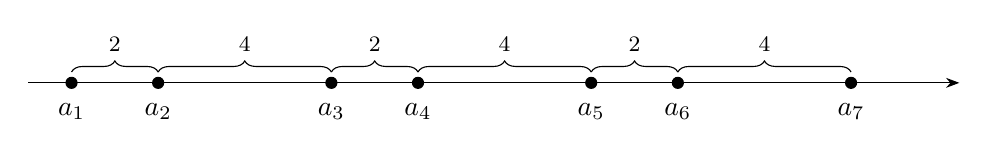
\begin{tikzpicture}[scale=0.55]
  \draw[-{Stealth}] (0,0) -- (21.5,0);
  \foreach \x in {1,3,7,9,13,15,19} \fill (\x,0) circle (4pt);
  \foreach \x/\l in {1/$a_1$,3/$a_2$,7/$a_3$,9/$a_4$,13/$a_5$,15/$a_6$,19/$a_7$}
    \node[below=4pt] at (\x,0) {\l};
  \foreach \a/\b/\g in {1/3/2,3/7/4,7/9/2,9/13/4,13/15/2,15/19/4}
    \draw[decorate,decoration={brace,amplitude=4pt}] (\a,0.25) -- (\b,0.25)
      node[midway,above=4pt] {\footnotesize $\g$};
\end{tikzpicture}
\end{center}

\begin{checkpoint}
(a) Write down the first six terms of a $(2,4)$-sequence that is \emph{not} eventually
periodic in its gaps --- that is, keep the gap pattern from ever settling into a
repeating cycle. Convince yourself you could continue it forever.
(b) Show that if $A$ is a $(d_1,d_2)$-sequence then
$a_1 + (n-1)\,d_1 \le a_n \le a_1 + (n-1)\,d_2$ for every $n$. (Add up the gaps.)
\end{checkpoint}

\subsection{Sumsets}

Our second ingredient is addition: we will be interested not in $A$ itself but in the
set of all numbers you can make by adding up $k$ members of $A$.

\begin{definition}[$k$-fold sumset]\label{def:sumset}
Let $A$ be a sequence and $k \ge 1$ an integer. The \emph{$k$-fold sumset} of $A$ is
\[
  kA \;:=\; \{\, x_1 + x_2 + \cdots + x_k \;:\; x_1, \dots, x_k \in A \,\},
\]
where the $x_i$ need \emph{not} be distinct --- you may use the same member of $A$
several times.
\end{definition}

Two warnings about this (standard) notation. First, $kA$ is \emph{not} the set
$\{k \cdot a : a \in A\}$ of multiples --- though it contains all of those (take
$x_1 = \cdots = x_k = a$). Second, repetitions are allowed: for
$A = \{1, 3, 7, \dots\}$ and $k = 3$, the sums $1+1+1 = 3$ and $1+1+7 = 9$ and
$3+7+7 = 17$ all belong to $3A$.

\begin{example}\label{ex:sumset-ap}
Let $A = \{5, 8, 11, 14, \dots\}$, the numbers of the form $5 + 3j$ with $j \ge 0$.
What is $3A$? Each element is a sum
\[
  (5 + 3j_1) + (5 + 3j_2) + (5 + 3j_3) \;=\; 15 + 3(j_1 + j_2 + j_3),
\]
and since $j_1 + j_2 + j_3$ can be any integer $\ge 0$, we get exactly
$3A = \{15, 18, 21, 24, \dots\}$: again an arithmetic progression with the same common
difference $3$, starting at $15$. This tidiness is special to arithmetic progressions
--- and, as we will see much later, it is precisely what makes them \emph{bad} at
dodging.
\end{example}

\begin{checkpoint}\label{chk:sumset}
(a) For $A = \{1, 3, 7, 9, 13, \dots\}$ of Example~\ref{ex:24seq}, list every element
of $3A$ up to $25$.
(b) Show that for any sequence $A$, the smallest element of $kA$ is $k a_1$.
(c) Show that if $A$ is a $(d_1,d_2)$-sequence, then between consecutive ``diagonal''
elements $k a_n$ and $k a_{n+1}$ of $kA$ the distance is at most $k d_2$.
\end{checkpoint}

\subsection{Lacunary sequences}

The sequence to be dodged grows \emph{multiplicatively}: each term is at least a fixed
multiple of the one before.

\begin{definition}[Lacunary sequence]\label{def:lacunary}
Let $r \ge 1$ be an integer. A sequence $B = \{b_1 < b_2 < \cdots\}$ is \emph{lacunary
with ratio $r$} if
\[
  b_{i+1} \;\ge\; r \, b_i \qquad \text{for every } i \ge 1.
\]
\end{definition}

\begin{example}
The powers $\{r, r^2, r^3, \dots\}$ are lacunary with ratio $r$ --- the minimal
example, growing as slowly as the definition allows. But a lacunary sequence need not
be this regular: $\{1, 7, 100, 1000, 10^{12}, \dots\}$ is lacunary with ratio $7$, as
long as every step multiplies by at least $7$. The word \emph{lacunary} comes from the
Latin \emph{lacuna}, a gap or hollow: on the number line, such a sequence is almost all
gap.
\end{example}

The picture to hold: a lacunary sequence with a large ratio is \emph{extremely sparse}.
Below any number $N$ it has at most about $\log_r N$ terms. Between consecutive terms
$b_i$ and $b_{i+1} \ge r b_i$ yawns an empty stretch $r$ times longer than everything
that came before. Sparseness is what should make $B$ \emph{easy} to dodge --- that is
the intuition the problem tests.

\begin{checkpoint}
Let $B$ be lacunary with ratio $r \ge 2$. Show that $b_i \ge b_1 \, r^{\,i-1}$ for all
$i$, and conclude that $B$ has at most $1 + \log_2 N$ terms below any $N \ge b_1$.
\end{checkpoint}

\subsection{The question, as a game}\label{sec:game}

We can now state the problem. Here it is verbatim, as recorded on
\texttt{erdosproblems.com} as problem 1112:

\begin{quote}
Let $1 \le d_1 < d_2$ and $k \ge 3$. Does there exist an integer $r$ such that if
$B = \{b_1 < \cdots\}$ is a lacunary sequence of positive integers with
$b_{i+1} \ge r b_i$ then there exists a sequence of positive integers
$A = \{a_1 < \cdots\}$ such that $d_1 \le a_{i+1} - a_i \le d_2$ for all $i \ge 1$ and
$(kA) \cap B = \emptyset$, where $kA$ is the $k$-fold sumset?
\end{quote}

Every phrase in this is now something we know. But sentences with three quantifiers
(``there exists $r$ \dots\ such that if [every] $B$ \dots\ then there exists $A$'')
are hard to hold in the head, so let us restate it as a \emph{game} between you and an
Adversary. The numbers $k \ge 3$ and $1 \le d_1 < d_2$ are fixed in advance and known
to both players.

\begin{enumerate}
\item \textbf{You} announce an integer $r$ --- once and for all.
\item \textbf{The Adversary}, knowing $r$, builds a lacunary sequence $B$ with ratio
      $r$: an infinite sequence with $b_{i+1} \ge r b_i$. The Adversary is infinitely
      clever and builds $B$ specifically to hurt you.
\item \textbf{You}, knowing $B$ completely, build a $(d_1,d_2)$-sequence $A$: a walk
      with steps in $[d_1, d_2]$.
\end{enumerate}

\noindent\textbf{You win} if $kA$ avoids $B$ entirely: no sum of $k$ members of $A$
ever equals a member of $B$. In symbols, $(kA) \cap B = \emptyset$.

The problem asks: \emph{do you have a winning strategy?} That is, is there a single
choice of $r$ such that, whatever $B$ the Adversary produces, you can answer with a
winning $A$?

The order of moves is the soul of the statement, so let us dwell on it.

\begin{itemize}
\item You choose $A$ \emph{after} seeing all of $B$. You may tailor your walk to the
      particular sequence you must dodge. (If instead you had to choose $A$ first, the
      Adversary would simply pick some element of $kA$ --- it is an infinite set ---
      and start $B$ there. You would lose always, and the problem would be boring.)
\item But you choose $r$ \emph{before} seeing $B$. One fixed $r$ must defeat every
      lacunary-ratio-$r$ sequence at once. Making $r$ enormous makes the Adversary's
      sequence extremely sparse --- intuitively, easier to dodge. The question is
      whether \emph{any} $r$, however large, is enough.
\end{itemize}

Why would this be hard? Your walk $A$ is dense --- steps at most $d_2$, so you have
lots of members --- and it is only $kA$, the $k$-fold sums, that must dodge $B$. The
tension: $A$'s gaps are \emph{bounded}, so $kA$ is forced to be rather evenly spread,
and an evenly spread set has a hard time missing even a very sparse one, because
``evenly spread'' means it shows up everywhere at every scale. Whether the $k$-fold
sums have enough slack to be steered around a sparse $B$ --- that is exactly what the
problem is asking, and the answer will turn out to hinge on a precise comparison
between $k$ and $d_2$.

\subsection{A first fight: tiny \texorpdfstring{$r$}{r} loses}\label{sec:first-fight}

To get blood flowing, let us play the game and prove something: announcing $r = 1$
loses. This tiny result will not be needed later, but it makes the rules concrete, and
it is our first complete proof.

\begin{proposition}\label{prop:r1}
Let $k \ge 3$ and $1 \le d_1 < d_2$. If you announce $r = 1$, the Adversary wins:
there is a lacunary sequence $B$ with ratio $1$ such that every $(d_1,d_2)$-sequence
$A$ has $(kA) \cap B \ne \emptyset$.
\end{proposition}

\begin{proof}
With $r = 1$ the lacunarity condition reads $b_{i+1} \ge b_i$, which any increasing
sequence satisfies. So the Adversary may play
\[
  B \;=\; \{1, 2, 3, 4, 5, \dots\},
\]
all positive integers. Now let $A$ be any $(d_1,d_2)$-sequence whatsoever. The sumset
$kA$ is not empty --- it contains, for instance, $k a_1$ (add $a_1$ to itself $k$
times), which is a positive integer, hence a member of $B$. So
$(kA) \cap B \ne \emptyset$: the Adversary wins.
\end{proof}

The same trivially covers $r \le 0$ (for $B$ positive, $b_{i+1} \ge r b_i$ is then no
constraint at all). So any winning $r$ must be at least $2$, and the real question
starts there: the problem page asks about ``an integer $r$'', and we now see this
means, in effect, an integer $r \ge 2$.

\begin{checkpoint}
Suppose you announce $r = 2$ and, feeling lazy, you resolve to always play an
arithmetic progression: $A = \{c, c+d, c+2d, \dots\}$ for some starting point $c$ and
fixed gap $d \in [d_1, d_2]$ of your choosing. Show that the Adversary can beat this
strategy. (Hint: Example~\ref{ex:sumset-ap} shows $kA$ is itself an arithmetic
progression --- it contains all sufficiently large multiples of $d$... at least when
$\gcd$-considerations cooperate. First try to see why the Adversary can defeat each
\emph{single} progression, then worry about defeating all of them with one $B$. The
second part is genuinely harder; we will meet it seriously in Part~III as the
``certificate trick''.)
\end{checkpoint}

\subsection{The answer}\label{sec:answer}

Here is the theorem this document proves. It answers the question completely, and the
answer is a genuine dichotomy: a sharp line through parameter space, with a winning
strategy on one side and a losing verdict on the other.

\begin{maintheorem}[The dichotomy]\label{thm:main-friendly}
Let $k \ge 3$ and $1 \le d_1 < d_2$ be integers.
\begin{enumerate}
\item \textup{(Existence.)} If $d_2 \ge k+1$, you have a winning strategy. In fact
      announcing any $r \ge 192\, d_2$ works: every lacunary $B$ with that ratio can
      be dodged by some $(d_1,d_2)$-sequence $A$ with $(kA) \cap B = \emptyset$.
\item \textup{(Non-existence, in a strong form.)} If $d_2 \le k$, no announcement
      wins. Worse: even if the fixed ratio $r$ is replaced by any prescribed sequence
      $r_1, r_2, r_3, \dots$ of lower bounds --- the Adversary now being required to
      satisfy $b_{i+1} \ge r_i\, b_i$ at every step, with the $r_i$ growing as fast as
      you like --- the Adversary can still build a \emph{single} sequence $B$ that
      defeats \emph{every} $(d_1,d_2)$-sequence $A$ at once.
\end{enumerate}
So the answer to Erd\H{o}s problem 1112 is: \emph{yes precisely when $d_2 \ge k+1$}.
\end{maintheorem}

Pause on how lopsided the two conclusions are. Above the threshold, one fixed ratio
$192\,d_2$ tames every lacunary $B$. Below it, the collapse is total: you may demand
$b_{i+1} \ge r_i b_i$ with $r_i = 10^{10^i}$ --- forcing $B$ to be unimaginably sparse
--- and still a single $B$ meets the $k$-fold sums of \emph{every} admissible walk.
Sparseness, which looked like your best friend in \S\ref{sec:game}, turns out to be
completely irrelevant below the threshold: no amount of it saves you.

Notice also what the threshold does \emph{not} depend on: $d_1$. Only the largest
allowed step $d_2$ matters, measured against the number of summands $k$. Why the
combination ``$d_2$ versus $k+1$''? That is the subject of the next section, where one
picture explains the whole dichotomy --- and the rest of the document is the long,
happy labor of making that picture rigorous.

\subsection{Map of the document}\label{sec:map-friendly}

\textbf{Part I} (\S\ref{sec:problem}--\ref{sec:picture}) states the problem and
gives the one picture --- windows of width $k$ striding at pace $\gamma$ --- from
which everything grows; \S\ref{sec:honest-list} turns that picture into an honest
ledger of four gaps, which the rest of the document closes. \textbf{Part II}
(\S\ref{sec:beatty}--\ref{sec:nested}) proves the existence half: floor toolbox,
Beatty walks, the safe/unsafe dial, the free-gap lemma, nested intervals, the
ratio $192\,d_2$. \textbf{Part III} (\S\ref{sec:cert}--\ref{sec:slot}) reduces
the non-existence half to walks (the certificate trick), then proves every
admissible walk tail-covering: easy cases first, then the two-letter campaign ---
band and sweep, the Morse--Hedlund classification, the Sturmian endgame --- and
finally the slot lemma, which prices the corner at exactly the subset-sum lemma.
\textbf{Part IV} (\S\ref{sec:sharp-intro}--\ref{sec:sharp-assembly}) proves that
lemma: machinery, reduction to the hard core, six branches. \textbf{Part V}
(\S\ref{sec:assembly-friendly}--\ref{sec:computer}) assembles the theorem and
explains the computer verification.

\emph{Three reading routes.} The \emph{spine}: \S\ref{sec:problem},
\S\ref{sec:picture}, then the Big idea boxes and theorem statements of each
part --- an afternoon, and you will know what is true and why it is plausible.
The \emph{existence route}: Parts I--II are self-contained and fully rigorous
--- a complete, checkable proof of the positive half in about twenty pages. The
\emph{whole climb}: everything in order; the two mini-courses
(\S\ref{sec:words}, \S\ref{sec:sturmian-course}) and Part~IV are steepest.
Checkpoints throughout are the footholds.

\emph{Correspondence with the research paper.} Part I $\leftrightarrow$ its
\S1; Part II $\leftrightarrow$ its \S2; Part III $\leftrightarrow$ its \S3;
Part IV $\leftrightarrow$ its \S4; Part V $\leftrightarrow$ its \S5--\S6 and
appendices. Every theorem here bears the same content as a numbered result
there (and through its Appendix~C, a machine-checked Lean declaration); this
document adds pedagogy, examples and checkpoints, and inherits all
authority from the parent.

%======================================================================

\section{The one picture that explains the threshold}\label{sec:picture}

Why should the dividing line fall at $d_2 = k+1$? Before any rigor, this section shows
you the picture from which the entire proof grows. Nothing here is officially part of
the proof --- everything will be re-done carefully later --- but every later section is
best read with this picture in mind. The section ends with an honest list of exactly
what the picture does \emph{not} establish; that list is the table of contents of the
rest of the document.

\subsection{Steady walks, and rounding error}\label{sec:steady}

Among all $(d_1,d_2)$-sequences, the simplest are the \emph{steady} ones: walks that
try to move at a constant average speed $\gamma$ per step. If $\gamma$ is an integer $d$,
that is an arithmetic progression, $a_i = c + i d$. But $\gamma$ need not be an
integer. To walk at average speed $\gamma = 3.5$, alternate steps of $3$ and $4$; and
in general, the canonical way to walk at any real speed $\gamma$ is to place your
$i$-th footfall at the integer just below $i\gamma$:
\[
  a_i \;=\; c + \lfloor i \gamma \rfloor \qquad (i = 1, 2, 3, \dots),
\]
where $c \ge 0$ is an integer offset and $\lfloor x \rfloor$ denotes the \emph{floor}
of $x$, the greatest integer $\le x$ (so $\lfloor 3.5 \rfloor = 3$,
$\lfloor 7 \rfloor = 7$). We will call this the \emph{Beatty walk} with slope $\gamma$
and offset $c$.\footnote{After Samuel Beatty, whose name is attached to sequences of
the form $\lfloor i\gamma \rfloor$. Part~II develops their basic properties from
scratch; here we only need the rough picture.}

\begin{example}\label{ex:beatty35}
Take $\gamma = 3.5$ and $c = 0$. Then $\lfloor 1 \cdot 3.5 \rfloor = 3$,
$\lfloor 2 \cdot 3.5 \rfloor = 7$, $\lfloor 3 \cdot 3.5 \rfloor = 10$, and so on:
\[
  A \;=\; \{3,\ 7,\ 10,\ 14,\ 17,\ 21,\ 24,\ 28,\ 31,\ 35,\ \dots\},
\]
with gaps $4, 3, 4, 3, 4, 3, \dots$ --- a perfectly legal $(d_1, 4)$-sequence for any
$d_1 \le 3$.
\end{example}

Now the question the whole problem turns on: \emph{where do the $k$-fold sums of a
steady walk live?} Take $k$ members of the walk, say with indices $i_1, \dots, i_k$,
and write $s := i_1 + \cdots + i_k$ for the index total. If there were no floors, the
sum would be exactly $kc + s\gamma$. Each floor rounds down by less than $1$ ---
$\lfloor x \rfloor$ always lies in the half-open interval $(x - 1,\ x]$ --- so $k$
floors together round down by less than $k$:
\[
  a_{i_1} + \cdots + a_{i_k}
  \;=\; kc + \sum_{t=1}^{k} \lfloor i_t \gamma \rfloor
  \;\in\; \big(\, kc + s\gamma - k,\ \; kc + s\gamma \,\big].
\]
Every $k$-fold sum therefore lands in a \emph{window} of width $k$ hanging just below
one of the values $kc + s\gamma$. As $s$ runs through the integers, these anchor
values march along the number line in equal strides of $\gamma$:

\begin{bigidea}
The $k$-fold sums of a steady walk of speed $\gamma$ are confined to windows of width
$k$, one hanging below each multiple of $\gamma$ (shifted by $kc$). The windows stride
along the line at pace $\gamma$. Everything --- both halves of the dichotomy ---
follows from comparing the stride $\gamma$ to the window width $k$.
\end{bigidea}

\begin{checkpoint}\label{chk:floors}
Prove the inequality just used: for any real numbers $x_1, \dots, x_k$,
\[
  x_1 + \cdots + x_k - k \;<\; \lfloor x_1 \rfloor + \cdots + \lfloor x_k \rfloor
  \;\le\; x_1 + \cdots + x_k .
\]
(Start from $x - 1 < \lfloor x \rfloor \le x$ for a single $x$, and add.)
\end{checkpoint}

\subsection{Above the threshold: daylight}\label{sec:daylight}

Suppose the stride exceeds the window width: $\gamma > k$. Then consecutive windows do
not touch --- between the end of one and the start of the next there is a stretch of
length $\gamma - k$ that no $k$-fold sum of the walk can ever reach. Call these
stretches \emph{daylight}. They recur forever, once per stride, making up a fixed
positive fraction of the number line at every scale.

\begin{figure}[t]
\centering
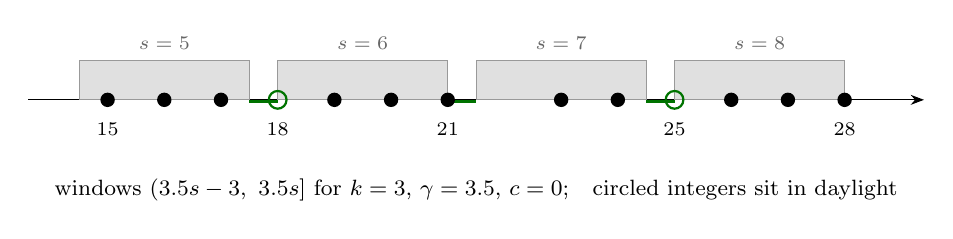
\begin{tikzpicture}[x=0.72cm, line width=0.4pt]
  % axis
  \draw[-{Stealth}] (13.6,0) -- (29.4,0);
  % windows (3.5s-3, 3.5s] for s=5..8, drawn as shaded boxes
  \foreach \lo/\hi/\s in {14.5/17.5/5, 18/21/6, 21.5/24.5/7, 25/28/8} {
    \fill[black!12] (\lo,0) rectangle (\hi,0.5);
    \draw[black!40] (\lo,0) rectangle (\hi,0.5);
    \node[font=\scriptsize, black!60] at ({(\lo+\hi)/2},0.72) {$s=\s$};
  }
  % daylight
  \foreach \lo/\hi in {17.5/18, 21/21.5, 24.5/25}
    \draw[green!45!black, very thick] (\lo,-0.02) -- (\hi,-0.02);
  % integer dots
  \foreach \x in {15,16,17,19,20,21,23,24,26,27,28} \fill (\x,0) circle (2.6pt);
  \foreach \x in {18,25} \draw[green!45!black, thick] (\x,0) circle (3.2pt);
  \foreach \x in {15,18,21,25,28} \node[below=5pt, font=\scriptsize] at (\x,0) {\x};
  % legend
  \node[font=\footnotesize, align=left] at (21.5,-1.15)
    {windows $(3.5s-3,\ 3.5s]$ for $k=3$, $\gamma=3.5$, $c=0$;\quad
     circled integers sit in daylight};
\end{tikzpicture}
\caption{The window picture for the walk of Example~\ref{ex:beatty35}. Each $3$-fold
sum lands in a shaded window; the integers $18$ and $25$ fall in the daylight between
windows, so they are \emph{unreachable}: no three members of $A$ sum to them. (The
window $(18,21]$ is open at its left end, which is why $18$ escapes.)}
\label{fig:windows}
\end{figure}

Figure~\ref{fig:windows} shows this for Example~\ref{ex:beatty35}, where $k = 3$ and
$\gamma = 3.5$: the windows are $(3.5s - 3,\ 3.5s]$ and the daylight stretches have
width $0.5$. The integer $25$ sits in daylight --- so no three members of that walk
sum to $25$, a fact you can (and should) also confirm by hand.

\begin{checkpoint}\label{chk:daylight35}
(a) Using the first ten terms listed in Example~\ref{ex:beatty35}, verify by direct
search that no three members of $A$ (repetitions allowed) sum to $18$ or to $25$.
(b) Explain why the window containment makes the search finite: any sum of three terms
involving a term $> 25$ is itself $> 25$.
(c) Find the next two unreachable integers after $25$.
\end{checkpoint}

Now the strategic point. When can an admissible walk have stride $\gamma > k$? The
steps available to us are integers between $d_1$ and $d_2$, so the fastest we can go is
$\gamma = d_2$, and to get a \emph{fractional} stride strictly between $k$ and an
achievable pair of step sizes we want to mix steps $d_2 - 1$ and $d_2$, giving any
speed $\gamma$ with $d_2 - 1 < \gamma < d_2$. Such a $\gamma$ exceeds $k$ exactly when
$d_2 - 1 \ge k$, that is, when
\[
  d_2 \;\ge\; k + 1 .
\]
There is the threshold, appearing for the first time --- not yet as a theorem, but as
the exact condition under which the daylight picture is available to us at all.

Above the threshold, then, here is the plan for winning the game. The daylight
stretches sit at predictable places, determined by the slope $\gamma$; \emph{turning
the dial $\gamma$ slides the whole ladder of windows}, and with it the daylight. Given
the Adversary's sequence $B$, we will tune $\gamma$ (and the offset $c$) so that every
single element of $B$ falls into daylight. One dial must dodge infinitely many targets
simultaneously --- that sounds ambitious, but the targets $b_i$ are lacunary, hence
ever sparser, and it will turn out (Part~II) that each successive target only forbids
a tiny range of dial positions, leaving plenty for the next. The tool that makes
``tiny'' precise is the \emph{free-gap lemma}, and the tool that finishes infinitely
many rounds of tuning is the \emph{nested interval theorem}. The mysterious ratio
$192\,d_2$ of Theorem~\ref{thm:main-friendly} is nothing deeper than the bookkeeping
constant that keeps each round of tuning from exhausting the dial room the previous
round left behind.

\subsection{Below the threshold: gridlock}\label{sec:gridlock}

Now suppose $d_2 \le k$, so every step is at most $k$ and every stride is at most $k$:
windows of width $k$ marching at pace $\gamma \le k$. Consecutive windows now overlap,
or at best touch. There is no daylight anywhere. The picture suggests that the
$k$-fold sums of such a walk eventually swallow everything in their path --- and for
steady \emph{integer} strides this is not merely a picture but a two-line calculation.

\begin{example}[Steady walks are hopeless]\label{ex:steady-hopeless}
Let $A$ be the arithmetic progression $a_i = c + i d$ with integer gap $d \le k$. A
$k$-fold sum is
\[
  (c + i_1 d) + \cdots + (c + i_k d) \;=\; kc + s d, \qquad s = i_1 + \cdots + i_k,
\]
and $s$ ranges over \emph{all} integers $\ge k$. So
\[
  kA \;=\; \{\, kc + sd \;:\; s \ge k \,\}:
\]
from $kc + kd$ onwards, $kA$ contains \emph{every} number that is $\equiv kc
\pmod d$. We say $kA$ contains a \emph{tail of a congruence class}. A set this fat
cannot dodge: however sparse the Adversary is forced to be, the class contains
arbitrarily large numbers, and the Adversary simply builds $B$ out of them ---
choosing each $b_{i+1}$ to be some member of the class beyond $r_i b_i$. Sparseness
costs the Adversary nothing, which is exactly the brutal flavor of part (2) of
Theorem~\ref{thm:main-friendly}.
\end{example}

\begin{checkpoint}
In Example~\ref{ex:steady-hopeless}, why does $s$ range over all integers $\ge k$ and
no others? (Show: each $i_t \ge 1$ gives $s \ge k$; conversely, realize any $s \ge k$
by choosing $i_1 = s - k + 1$ and $i_2 = \cdots = i_k = 1$.) Note this uses
repetitions --- Definition~\ref{def:sumset} earning its keep.
\end{checkpoint}

So a walk that wants to survive below the threshold must \emph{wobble}: vary its
steps, forever, in a way that never settles into an arithmetic progression. The entire
difficulty of the non-existence half is the question: \emph{can clever wobbling
recreate daylight?} The window picture pushes toward ``no'' --- wobbling changes where
the windows sit but not their width, and there is no room between them --- but the
picture reasons about steady walks, and a wobbling walk has no single stride $\gamma$.
That gap in the reasoning is not small print. Closing it is most of this document.

\subsection{What the picture does not prove}\label{sec:honest-list}

Here is the honest ledger --- four gaps between the picture and the theorem, and where
each one is closed.

\begin{enumerate}
\item \emph{Above the threshold, one dial setting must defeat all of $B$ at once.}
      The daylight argument dodges one target at a time; to dodge every $b_i$
      simultaneously we tune $\gamma$ through infinitely many rounds and must show the
      dial room never runs out. This is Part~II: the free-gap lemma
      (\S\ref{sec:freegap}) and the nested-interval construction
      (\S\ref{sec:nested}), yielding the explicit ratio $192\,d_2$.
\item \emph{Below the threshold, one $B$ must defeat all walks at once.}
      Example~\ref{ex:steady-hopeless} beats each steady walk with a $B$ built from
      \emph{its} congruence class --- but different walks use different classes, and
      the theorem demands a single $B$ that beats every admissible walk. The device
      that accomplishes this is the \emph{certificate trick} (\S\ref{sec:cert}), a
      diagonalization.
\item \emph{Below the threshold, wobbling walks must be shown hopeless too.} The plan:
      show every admissible walk's sumset contains a tail of a congruence class
      (``tail-covering''), by classifying how a walk can wobble --- the analysis of
      \emph{gap words} occupying \S\S\ref{sec:alphabet}--\ref{sec:slot}. The delicate
      walks are those that wobble between two step sizes as evenly and aperiodically
      as possible; these are the \emph{Sturmian} walks, and taming them
      (\S\S\ref{sec:sturmian-course}--\ref{sec:sturmian-endgame}) is the deepest water
      in the document.
\item \emph{The corner $d_2 = k$ is razor-thin.} When the largest step equals $k$
      exactly, the windows touch without overlapping, and the walk has just barely too
      little room; converting ``barely'' into a proof costs a genuinely new piece of
      finite mathematics about subset sums, stated in \S\ref{sec:sharp-intro} and
      proved across Part~IV.
\end{enumerate}

One more promissory note. In Example~\ref{ex:steady-hopeless} the offset ``$kc$''
depended on the walk, and in gap~(2) we waved at defeating all offsets and classes
simultaneously; when we do this properly, the notion of \emph{tail-covering} will be
defined to absorb all of it. From here on, the document simply executes the ledger:
Part~II closes gap~(1); Part~III closes gaps~(2) and~(3), reducing the corner case to
a finite lemma; Part~IV proves that lemma, closing gap~(4); Part~V assembles the
theorem and describes the computer verification.

%======================================================================
\part{Existence: winning when \texorpdfstring{$d_2 \ge k+1$}{d2 >= k+1}}
%======================================================================

\section{Floors and Beatty walks}\label{sec:beatty}

Part~II proves the existence half of the dichotomy: if $d_2 \ge k+1$, announcing
$r = 192\,d_2$ wins the game. The plan was sketched in \S\ref{sec:daylight}; from here
on we execute it rigorously. \textbf{Standing assumptions for all of Part~II:} $k$,
$d_1$, $d_2$ are integers with
\[
  k \ge 2, \qquad 1 \le d_1 < d_2, \qquad d_2 \ge k + 1 .
\]
(The problem poses $k \ge 3$, but the existence proof works verbatim from $k = 2$, so
we prove the slightly more general statement at no extra cost. Note $d_2 \ge 3$
follows.)

This section builds the two tools everything else stands on: the floor function, and
the fact that a Beatty walk with slope between $d_2 - 1$ and $d_2$ is a legal
$(d_1,d_2)$-sequence.

\subsection{The floor function}

\begin{definition}[Floor]\label{def:floor}
For a real number $x$, the \emph{floor} $\lfloor x \rfloor$ is the unique integer $m$
satisfying
\[
  m \;\le\; x \;<\; m + 1 .
\]
\end{definition}

So $\lfloor 3.5 \rfloor = 3$, $\lfloor 7 \rfloor = 7$, and (watch this one)
$\lfloor -0.5 \rfloor = -1$: the floor is the integer just \emph{below} $x$ (or $x$
itself), not ``the integer part''. That an integer $m \le x < m+1$ exists is visually
clear --- walk down the number line from above $x$ until you first pass an integer ---
and we take it as known; but uniqueness deserves its one-line proof: if
$m \le x < m+1$ and $m' \le x < m'+1$ with, say, $m < m'$, then $m + 1 \le m'$ (they
are integers), so $x < m + 1 \le m' \le x$, a contradiction.

Everything we ever use about floors is in the next lemma.

\begin{lemma}[Floor toolbox]\label{lem:floor-toolbox}
For all real $x, y$ and every integer $n$:
\begin{enumerate}
\item $x - 1 \;<\; \lfloor x \rfloor \;\le\; x$;
\item $\lfloor x + n \rfloor = \lfloor x \rfloor + n$;
\item if $x \le y$ then $\lfloor x \rfloor \le \lfloor y \rfloor$;
\item for reals $x_1, \dots, x_k$:\quad
      $x_1 + \cdots + x_k - k \;<\; \lfloor x_1 \rfloor + \cdots + \lfloor x_k \rfloor
       \;\le\; x_1 + \cdots + x_k$.
\end{enumerate}
\end{lemma}

\begin{proof}
Write $m = \lfloor x \rfloor$, so $m \le x < m+1$ by definition.

(1) The right inequality is $m \le x$ directly; the left is $x < m + 1$ rearranged.

(2) The integer $m + n$ satisfies $m + n \le x + n < (m+n) + 1$, which is exactly the
defining property of $\lfloor x + n \rfloor$; by uniqueness,
$\lfloor x+n \rfloor = m + n$.

(3) Suppose $x \le y$. Then $\lfloor x \rfloor \le x \le y$, so $\lfloor x \rfloor$
is an integer $\le y$. But $\lfloor y \rfloor$ is the \emph{greatest} integer $\le y$:
any integer $m' \le y$ has $m' \le \lfloor y \rfloor$, since otherwise
$m' \ge \lfloor y \rfloor + 1 > y$. Hence $\lfloor x \rfloor \le \lfloor y \rfloor$.

(4) Add the $k$ instances of (1): summing $x_t - 1 < \lfloor x_t \rfloor \le x_t$ over
$t = 1, \dots, k$ gives the claim. (This is Checkpoint~\ref{chk:floors}, now on the
official record.)
\end{proof}

\begin{checkpoint}
(a) Compute $\lfloor 5.999 \rfloor$, $\lfloor -3 \rfloor$, $\lfloor -3.01 \rfloor$.
(b) Show by example that $\lfloor x + y \rfloor$ is \emph{not} always
$\lfloor x \rfloor + \lfloor y \rfloor$ --- and prove that it always equals
$\lfloor x \rfloor + \lfloor y \rfloor$ or $\lfloor x \rfloor + \lfloor y \rfloor + 1$.
(c) Where does the proof of Lemma~\ref{lem:floor-toolbox}(2) break if $n$ is not an
integer?
\end{checkpoint}

\subsection{Beatty walks, officially}

\begin{definition}[Beatty walk]\label{def:beatty-walk}
For a real number $\gamma > 1$ and an integer $c \ge 0$, the \emph{Beatty walk} with
slope $\gamma$ and offset $c$ is the sequence
\[
  A_{\gamma,c} \;:=\; \{\, c + \lfloor i \gamma \rfloor \;:\; i = 1, 2, 3, \dots \,\},
  \qquad \text{i.e.} \quad a_i = c + \lfloor i\gamma \rfloor .
\]
\end{definition}

We met $A_{3.5,\,0} = \{3, 7, 10, 14, 17, 21, \dots\}$ in
Example~\ref{ex:beatty35}. One more, with a slope that is not a half-integer: for
$\gamma = \tfrac{10}{3}$ and $c = 0$,
\[
  \lfloor \tfrac{10}{3} \rfloor = 3,\ \
  \lfloor \tfrac{20}{3} \rfloor = 6,\ \
  \lfloor \tfrac{30}{3} \rfloor = 10,\ \
  \lfloor \tfrac{40}{3} \rfloor = 13,\ \dots
\]
so $A_{10/3,\,0} = \{3, 6, 10, 13, 16, 20, 23, 26, 30, \dots\}$, with gap pattern
$3, 4, 3, 3, 4, 3, 3, 4, \dots$: the gap $4$ arrives once every three steps, keeping
the average speed at exactly $\tfrac{10}{3}$.

The single structural fact we need is that a Beatty walk's gaps take at most two
values, and we can say which ones.

\begin{lemma}[Two-value gaps]\label{lem:two-gaps}
Let $\gamma > 1$ be real. Every gap of the Beatty walk $A_{\gamma,c}$ lies in
$\{\lfloor \gamma \rfloor,\ \lfloor \gamma \rfloor + 1\}$:
\[
  \lfloor (i+1)\gamma \rfloor - \lfloor i\gamma \rfloor
  \;\in\; \{\lfloor \gamma \rfloor,\ \lfloor \gamma \rfloor + 1\}
  \qquad \text{for every } i \ge 1 .
\]
\end{lemma}

\begin{proof}
The offset $c$ cancels from every gap, so consider
$g := \lfloor (i+1)\gamma \rfloor - \lfloor i\gamma \rfloor$, a difference of two
integers, hence an integer. We trap it in an open interval of length $2$. By
Lemma~\ref{lem:floor-toolbox}(1),
\[
  \lfloor (i+1)\gamma \rfloor \le (i+1)\gamma
  \quad\text{and}\quad
  \lfloor i\gamma \rfloor > i\gamma - 1,
\]
so $g < (i+1)\gamma - (i\gamma - 1) = \gamma + 1$. Similarly
$\lfloor (i+1)\gamma \rfloor > (i+1)\gamma - 1$ and $\lfloor i\gamma \rfloor \le
i\gamma$ give $g > \gamma - 1$. So $g$ is an integer with
\[
  \gamma - 1 \;<\; g \;<\; \gamma + 1 .
\]
Which integers lie strictly between $\gamma - 1$ and $\gamma + 1$? Only
$\lfloor \gamma \rfloor$ and $\lfloor \gamma \rfloor + 1$ can. To see this, split on
whether $g \le \gamma$ or $g > \gamma$.
\begin{itemize}
\item If $g \le \gamma$: then $g$ is an integer $\le \gamma$, so
      $g \le \lfloor \gamma \rfloor$ ($\lfloor \gamma \rfloor$ being the greatest
      such). On the other hand $\lfloor \gamma \rfloor \le \gamma$ gives
      $\lfloor \gamma \rfloor - 1 \le \gamma - 1 < g$. So
      $\lfloor \gamma \rfloor - 1 < g \le \lfloor \gamma \rfloor$, and the only
      integer in that range is $g = \lfloor \gamma \rfloor$.
\item If $g > \gamma$: then $g - 1$ is an integer with
      $\gamma - 1 < g - 1 < \gamma$, so the previous case applies to $g - 1$ and
      yields $g - 1 = \lfloor \gamma \rfloor$, i.e.\ $g = \lfloor \gamma \rfloor + 1$.
\end{itemize}
\end{proof}

(If $\gamma$ is an integer, only the value $\lfloor \gamma \rfloor = \gamma$ actually
occurs, and the walk is an arithmetic progression --- Checkpoint below. For
non-integer $\gamma$, both values occur infinitely often, though we will not need
that.)

\subsection{Beatty walks are admissible}

Now aim the slope at the top of our permitted window.

\begin{proposition}[Admissibility]\label{prop:beatty-admissible}
Let $\gamma$ be any real number with $d_2 - 1 < \gamma < d_2$, and $c \ge 0$ any
integer. Then $A_{\gamma,c}$ is a $(d_1,d_2)$-sequence.
\end{proposition}

\begin{proof}
Three things to check: the terms are positive, the sequence is strictly increasing,
and the gaps lie in $[d_1, d_2]$.

Since $d_2 - 1 < \gamma < d_2$ and $d_2 - 1, d_2$ are integers, the defining property
of the floor gives $\lfloor \gamma \rfloor = d_2 - 1$. By
Lemma~\ref{lem:two-gaps}, every gap of $A_{\gamma,c}$ is $d_2 - 1$ or $d_2$. Both lie
in $[d_1, d_2]$: indeed $d_1 \le d_2 - 1$ because $d_1 < d_2$ are integers. As
$d_2 \ge k + 1 \ge 3$, every gap is at least $2 > 0$, so the sequence is strictly
increasing; and its first term is $a_1 = c + \lfloor \gamma \rfloor \ge 0 + (d_2 - 1)
\ge 2 > 0$. All three checks pass.
\end{proof}

Two remarks worth pausing on. First, \emph{the slope may be rational}: nothing
anywhere in Part~II needs $\gamma$ irrational, and the final winning slope will simply
be some real number produced by the nested-interval theorem --- we will neither know
nor care whether it is rational. Second, notice how little of the freedom of
$(d_1,d_2)$-sequences we are using: only steps $d_2 - 1$ and $d_2$, the two largest.
The lower bound $d_1$ plays no role beyond $d_1 \le d_2 - 1$, which is automatic. This
is the promised explanation of why $d_1$ is absent from the threshold: the existence
strategy never has any reason to take a small step.

\begin{checkpoint}
(a) Show that if $\gamma = d$ is an integer, $A_{d,c}$ is the arithmetic progression
$c + d,\ c + 2d,\ c + 3d, \dots$
(b) For $\gamma = \tfrac{7}{2}$, which $i$ have gap $g_i = 4$ and which have $3$? Find
the pattern and prove it. (Hint: $\lfloor (i+1)\gamma\rfloor - \lfloor i\gamma\rfloor$
depends on whether $i$ is even or odd.)
(c) Show that for any real $\gamma > 1$, among the first $n$ gaps of $A_{\gamma,c}$,
the number of gaps equal to $\lfloor\gamma\rfloor + 1$ is
$\lfloor (n+1)\gamma \rfloor - \lfloor \gamma \rfloor - n\lfloor\gamma\rfloor$.
(Telescope the sum of the gaps.)
\end{checkpoint}

\section{Where the \texorpdfstring{$k$}{k}-fold sums live}\label{sec:windows}

This section turns the window picture of \S\ref{sec:picture} into theorems, and then
performs the change of viewpoint on which the whole existence proof runs: instead of
asking \emph{which numbers} the walk's sums can reach, we ask \emph{which dial
positions $\gamma$} are safe for a given target. By the end of the section, dodging a
single element of $B$ will be a clean geometric condition on $\gamma$ alone.

\subsection{The window containment}

\begin{proposition}[Windows]\label{prop:windows}
Let $\gamma > 1$ be real, $c \ge 0$ an integer, and $k \ge 1$. Then
\[
  k A_{\gamma,c} \;\subseteq\; \bigcup_{s \ge k}
     \big(\, kc + s\gamma - k,\ \; kc + s\gamma \,\big],
\]
the union over integers $s \ge k$.
\end{proposition}

\begin{proof}
A member of $k A_{\gamma,c}$ is a sum of $k$ terms of the walk, say with indices
$i_1, \dots, i_k \ge 1$ (repetitions allowed):
\[
  \sum_{t=1}^{k} \big( c + \lfloor i_t \gamma \rfloor \big)
  \;=\; kc + \sum_{t=1}^{k} \lfloor i_t \gamma \rfloor .
\]
Set $s := i_1 + \cdots + i_k$; since each $i_t \ge 1$, we have $s \ge k$. By the
sum-of-floors bound (Lemma~\ref{lem:floor-toolbox}(4)) applied to the numbers
$x_t = i_t \gamma$, whose sum is $s\gamma$,
\[
  s\gamma - k \;<\; \sum_{t=1}^{k} \lfloor i_t \gamma \rfloor \;\le\; s\gamma ,
\]
so the member lies in $(kc + s\gamma - k,\ kc + s\gamma]$.
\end{proof}

Alongside the windows we record where the sums \emph{start}: nothing in
$k A_{\gamma,c}$ is small.

\begin{lemma}[Sums start high]\label{lem:min-sum}
If $d_2 - 1 < \gamma < d_2$, the smallest element of $k A_{\gamma,c}$ is
$k(c + d_2 - 1)$. In particular every integer $b \le kc$ satisfies
$b \notin k A_{\gamma,c}$: targets at or below $kc$ are dodged automatically.
\end{lemma}

\begin{proof}
Every term of the walk is at least its first term $a_1 = c + \lfloor \gamma \rfloor =
c + d_2 - 1$, so every $k$-fold sum is at least $k a_1 = k(c + d_2 - 1)$ --- and this
value is attained, by summing $a_1$ with itself $k$ times. Finally
$k(c + d_2 - 1) > kc$, since $d_2 \ge 2$.
\end{proof}

\subsection{The avoidance criterion}

Fix a target $b > kc$ that we wish to keep out of $k A_{\gamma,c}$, and write
\[
  t \;:=\; b - kc \;\ge\; 1
\]
for the \emph{shifted target}. Subtracting $kc$ throughout,
Proposition~\ref{prop:windows} says: if $b \in kA_{\gamma,c}$, then
$t \in (s\gamma - k,\ s\gamma]$ for some integer $s \ge k$ --- equivalently,
$s\gamma \in [\,t,\ t + k)$ for some $s \ge k$. Turning this around gives the
criterion we will use forever after.

\begin{definition}[Safe slope]\label{def:safe}
Let $t \ge 1$ be an integer. A real $\gamma > 0$ is \emph{safe for $t$} if
\[
  s\gamma \;\notin\; [\,t,\ t + k\,] \qquad \text{for every integer } s \ge 1 .
\]
\end{definition}

\begin{proposition}[Avoidance criterion]\label{prop:criterion}
Let $d_2 - 1 < \gamma < d_2$, let $c \ge 0$, and let $b > kc$ be an integer. If
$\gamma$ is safe for $t = b - kc$, then $b \notin k A_{\gamma,c}$.
\end{proposition}

\begin{proof}
Contrapositive. If $b \in k A_{\gamma,c}$, the discussion above produces an integer
$s \ge k \ge 1$ with $s\gamma \in [t, t+k) \subseteq [t, t+k]$, so $\gamma$ is not
safe for $t$.
\end{proof}

Look closely: Definition~\ref{def:safe} demands \emph{more} than the proof of
Proposition~\ref{prop:criterion} needs, in two ways, and both are deliberate.

\begin{itemize}
\item It forbids $s\gamma \in [t, t+k]$ for \emph{all} $s \ge 1$, though only
      $s \ge k$ can actually occur in a window. Ruling out extra values of $s$ is a
      stronger demand on $\gamma$ --- harmless for the conclusion, and it frees every
      later argument from tracking which $s$ are realizable.
\item It uses the \emph{closed} interval $[t, t+k]$, though the windows are half-open.
      Again this only makes ``safe'' harder to achieve, never easier --- and closed
      intervals are more comfortable to work with (their endpoints belong to them, so
      ``the least $s$ with\dots'' arguments have no edge cases).
\end{itemize}

The cost of this generosity is real but affordable: some slopes that would in fact
dodge $b$ are not certified safe. You will meet a concrete instance in
Checkpoint~\ref{chk:conservative} --- the walk of Example~\ref{ex:beatty35} really
does miss $25$, yet the criterion declines to vouch for it. We simply will not care:
the free-gap lemma of \S\ref{sec:freegap} finds slopes that pass even the stricter
test.

\begin{bigidea}
For a Beatty walk, ``the sum of $k$ members never equals $b$'' has become a statement
about the dial position alone: no multiple $s\gamma$ may land in the closed window
$[t, t+k]$, where $t = b - kc$. The game of dodging an infinite sequence $B$ is now a
game of placing one real number $\gamma$ clear of infinitely many forbidden zones.
\end{bigidea}

\begin{checkpoint}\label{chk:conservative}
Take the walk of Example~\ref{ex:beatty35}: $\gamma = 3.5$, $c = 0$, $k = 3$.
(a) Show that $\gamma$ is \emph{not} safe for $t = 25$: find the integer $s$ with
$3.5\,s \in [25, 28]$.
(b) Yet $25 \notin 3A$ (Checkpoint~\ref{chk:daylight35}). Explain, using the half-open
window $(25, 28]$, why the point $3.5 \cdot 8 = 28$ landing exactly on the closed
window's right endpoint does not put $25$ into $3A$ --- so the criterion's verdict is
merely conservative, not wrong.
(c) Stronger: show that \emph{no} integer $t \ge 1$ is safe for $\gamma = 3.5$.
(Consider the smallest multiple $u$ of $3.5$ with $u \ge t$; multiples of $3.5$ are
integers or half-integers, so show $u \le t + 3$.) So at this particular slope the
criterion certifies nothing at all --- even though the walk misses $18, 25, 32,
\dots$ The slopes the free-gap lemma will select are precisely engineered to avoid
this fate.
(d) By listing the unsafe intervals $[\frac{46}{s}, \frac{49}{s}]$ that meet
$(3, 4)$, find a slope that \emph{is} safe for $t = 46$, and verify your slope
directly against $s = 12$ and $s = 13$.
\end{checkpoint}

\subsection{The dial, and its unsafe zones}\label{sec:dial}

Fix the shifted target $t$ and look at the condition of
Definition~\ref{def:safe} from the dial's point of view. For each single $s \ge 1$,
\[
  s\gamma \in [t,\ t+k]
  \quad\Longleftrightarrow\quad
  \gamma \in \Big[\, \frac{t}{s},\ \frac{t+k}{s} \,\Big] ,
\]
so the slopes ruled out by index $s$ form a closed interval, and $\gamma$ is safe for
$t$ exactly when it avoids the \emph{unsafe set}
\[
  U_t \;:=\; \bigcup_{s \ge 1} \Big[\, \frac{t}{s},\ \frac{t+k}{s} \,\Big] .
\]
As $s$ grows, these unsafe intervals march down the dial toward $0$, shrinking as they
go (both endpoints are proportional to $1/s$). Figure~\ref{fig:dial} shows the portion
of $U_{100}$ near the dial region we shop in, for $k = 3$.

\begin{figure}[t]
\centering
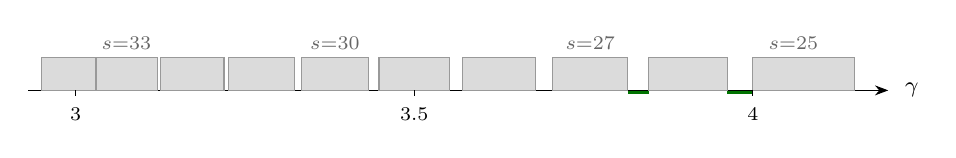
\begin{tikzpicture}[x=8.6cm, line width=0.4pt]
  % axis from 2.95 to 4.18
  \draw[-{Stealth}] (2.93,0) -- (4.20,0);
  \node[font=\footnotesize] at (4.235,0) {$\gamma$};
  % unsafe intervals [100/s, 103/s]
  \foreach \lo/\hi in {4.000/4.150, 3.846/3.962, 3.704/3.815, 3.571/3.679,
                       3.448/3.552, 3.333/3.433, 3.226/3.323, 3.125/3.219,
                       3.030/3.121, 2.950/3.029} {
    \fill[black!14] (\lo,0) rectangle (\hi,0.42);
    \draw[black!40] (\lo,0) rectangle (\hi,0.42);
  }
  \foreach \x/\s in {4.06/25, 3.76/27, 3.383/30, 3.075/33}
    \node[font=\scriptsize, black!60] at (\x,0.60) {$s{=}\s$};
  % safe gaps highlighted
  \foreach \lo/\hi in {3.962/4.000, 3.815/3.846}
    \draw[green!45!black, very thick] (\lo,-0.03) -- (\hi,-0.03);
  % ticks
  \foreach \x/\l in {3.0/3, 3.5/3.5, 4.0/4}
    { \draw (\x,0) -- (\x,-0.07); \node[below=3pt, font=\scriptsize] at (\x,0) {\l}; }
\end{tikzpicture}
\caption{The unsafe set $U_{100}$ for $k=3$, on the stretch $2.95 \le \gamma \le
4.18$ of the dial: the interval $[\frac{100}{s}, \frac{103}{s}]$ for
$s = 25, 26, \dots, 34$. Safe gaps (two are marked) open up between consecutive
unsafe intervals, wider toward the right; toward the left the intervals crowd
together and, below $\gamma = 3 = k$, merge into a solid unsafe block
(Proposition~\ref{prop:no-safety-below-k}).}
\label{fig:dial}
\end{figure}

Two features of this picture are the pivot of the whole story. First, the safe gaps
--- the white space between consecutive unsafe intervals --- \emph{exist} in the
region $\gamma > k$, and we will learn to find them (\S\ref{sec:freegap}). Second,
below $\gamma = k$ there is nothing to find:

\begin{proposition}[No safety below $k$]\label{prop:no-safety-below-k}
Let $t \ge 1$ be an integer. Every real $\gamma$ with $0 < \gamma \le k$ is unsafe
for $t$.
\end{proposition}

\begin{proof}
We must find an integer $s \ge 1$ with $s\gamma \in [t, t+k]$, i.e.\ with
\[
  s \;\in\; \Big[\, \frac{t}{\gamma},\ \frac{t+k}{\gamma} \,\Big] .
\]
This is a real interval of length $k/\gamma \ge 1$, so it contains an integer $s$
(between any two reals at distance $\ge 1$ there is an integer:
$s = \lfloor t/\gamma \rfloor + 1$ works, as it satisfies
$t/\gamma < s \le t/\gamma + 1 \le (t+k)/\gamma$). That integer is positive, since
$s > t/\gamma > 0$.
\end{proof}

This is the threshold, seen from the dial. A walk whose stride is at most $k$ cannot
be certified to dodge \emph{anything}: every single target's unsafe set swallows the
entire dial region $(0, k]$. Our standing assumption $d_2 \ge k+1$ is exactly what
places the shopping district $(d_2 - 1,\ d_2)$ of
Proposition~\ref{prop:beatty-admissible} inside the living zone $\gamma > k$. (That
the picture ``no safety below $k$'' hardens into the actual non-existence theorem
below the threshold --- not merely a failure of this particular criterion --- is the
business of Parts III and IV.)

What remains for the existence half is quantitative: given the target $t$, \emph{how
wide} are the safe gaps near the top of the dial, and how little of the dial does each
new target destroy? That is the free-gap lemma, to which we now turn.

\begin{checkpoint}
Let $k = 3$ and $t = 20$. (a) List the unsafe intervals
$[\frac{20}{s}, \frac{23}{s}]$ that meet the dial stretch $(3, 4)$, and conclude that
the safe slopes there form exactly the two gaps
$\big(\tfrac{23}{7}, \tfrac{20}{6}\big)$ and $\big(\tfrac{23}{6}, 4\big)$.
(b) Pick a slope in one of them and write down the first eight terms of a
$(1,4)$-walk none of whose $3$-fold sums equals $20 + 3c$ for your chosen offset $c$.
\end{checkpoint}

\begin{checkpoint}\label{chk:overlap}
Show that the unsafe intervals for indices $s$ and $s+1$ overlap or touch --- that
is, $\frac{t+k}{s+1} \ge \frac{t}{s}$ --- if and only if $s \ge t/k$. (This is the
precise sense in which the unsafe intervals ``merge into a solid block'' at the left
of Figure~\ref{fig:dial}: from $s = \lceil t/k \rceil$ onward, consecutive intervals
chain together without gaps.)
\end{checkpoint}

\section{The free-gap lemma}\label{sec:freegap}

We now build the engine of the existence proof. The task left over from
\S\ref{sec:dial}: given a target $t$, find a safe stretch of dial --- and find it
\emph{quantitatively}, because we will have to do this infinitely often, once per
element of $B$, each time inside whatever room the previous rounds left us. The lemma
of this section says: inside any dial interval that is not too narrow (compared to
$1/t$), there is a safe subinterval that is not too much narrower. The two ``not
too''s are what the constant $192$ will be made of in \S\ref{sec:nested}.

One more tool for the toolbox first.

\begin{definition}[Ceiling]\label{def:ceiling}
For a real $x$, the \emph{ceiling} $\lceil x \rceil$ is the unique integer $m$ with
$m - 1 < x \le m$ --- the least integer $\ge x$. (Uniqueness: as for the floor. Note
$\lceil x \rceil = \lfloor x \rfloor$ when $x$ is an integer, and
$\lfloor x \rfloor + 1$ otherwise.)
\end{definition}

\subsection{The statement}

\begin{lemma}[Free gap]\label{lem:freegap-friendly}
Let $t \ge 32\,d_2^{\,2}$ be an integer, and let $I = [lo,\ hi]$ be a closed real
interval with
\[
  I \;\subseteq\; \big[\, d_2 - \tfrac12,\ d_2 \,\big]
  \qquad\text{and}\qquad
  |I| \;=\; hi - lo \;\ge\; \frac{4 d_2^{\,2}}{t} .
\]
Then $I$ contains a closed subinterval $I'$ with
\[
  |I'| \;\ge\; \frac{d_2}{48\,t}
\]
such that \emph{every} $\gamma \in I'$ is safe for $t$ (Definition~\ref{def:safe}):
$s\gamma \notin [t,\ t+k]$ for every integer $s \ge 1$.
\end{lemma}

Read the shape of this before the proof. The input interval must have width at least
$4d_2^2/t$; the output is guaranteed width at least $d_2/(48t)$. Both scale like
$1/t$: a bigger target is dodged with proportionally finer dial adjustments. The
ratio between them,
\[
  \frac{4 d_2^{\,2}/t}{d_2/(48t)} \;=\; 192\, d_2 ,
\]
is the number of times the output of one round fits into the input the next round
demands --- hold that thought until \S\ref{sec:nested}, where it becomes the theorem's
constant.

\subsection{The idea: name one gap, count nothing}

The unsafe set $U_t = \bigcup_{s\ge1} [t/s,\ (t+k)/s]$ is an infinite union, and a
first instinct is to estimate how many of its intervals meet $I$ and how much room
they eat. That accounting can be made to work, but there is something better: we can
point at \emph{one specific gap} between two \emph{specific} consecutive unsafe
intervals, and prove that this single gap already avoids every unsafe interval at
once, has the width we need, and sits inside $I$. No counting, no union bounds ---
three clean checks on one explicitly named object.

Which gap? Look at Figure~\ref{fig:dial} again: near the top of the dial the unsafe
intervals are the sparsest and the gaps the widest, so we aim as high in $I$ as
possible. Let
\[
  s_1 \;:=\; \Big\lceil \frac{t}{hi} \Big\rceil
  \qquad\text{(the least integer $s$ with } t/s \le hi\text{)} ,
\]
so that the unsafe interval of index $s_1$ is the highest-placed one whose left
endpoint has not yet escaped past the top of $I$. Our gap is the space just below
that interval and just above the next one:
\[
  L \;:=\; \frac{t+k}{s_1 + 1}, \qquad
  R \;:=\; \frac{t}{s_1}, \qquad
  J \;:=\; (L,\ R)
\]
--- the open interval between the right end of unsafe interval $s_1 + 1$ and the left
end of unsafe interval $s_1$.

\begin{center}
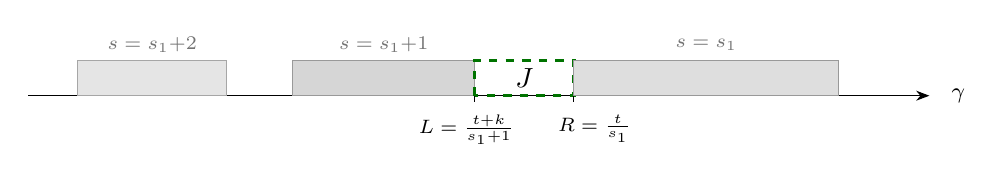
\begin{tikzpicture}[x=1.05cm, line width=0.4pt]
  \draw[-{Stealth}] (-0.3,0) -- (10.6,0);
  \node[font=\footnotesize] at (10.95,0) {$\gamma$};
  \fill[black!10] (0.3,0) rectangle (2.1,0.45);
  \draw[black!35] (0.3,0) rectangle (2.1,0.45);
  \node[font=\scriptsize, black!55] at (1.2,0.65) {$s = s_1{+}2$};
  \fill[black!16] (2.9,0) rectangle (5.1,0.45);
  \draw[black!40] (2.9,0) rectangle (5.1,0.45);
  \node[font=\scriptsize, black!55] at (4.0,0.65) {$s = s_1{+}1$};
  \draw[green!45!black, dashed, very thick] (5.1,0) rectangle (6.3,0.45);
  \node at (5.7,0.225) {$J$};
  \fill[black!13] (6.3,0) rectangle (9.5,0.45);
  \draw[black!40] (6.3,0) rectangle (9.5,0.45);
  \node[font=\scriptsize, black!55] at (7.9,0.65) {$s = s_1$};
  \draw (5.1,0) -- (5.1,-0.08); \node[below=3pt,font=\scriptsize] at (5.0,-0.02) {$L = \frac{t+k}{s_1+1}$};
  \draw (6.3,0) -- (6.3,-0.08); \node[below=3pt,font=\scriptsize] at (6.55,-0.02) {$R = \frac{t}{s_1}$};
\end{tikzpicture}
\end{center}

\subsection{Three checks}

Throughout, remember the standing facts: $2 \le k \le d_2 - 1$ (from
$d_2 \ge k+1$), $d_2 \ge 3$, $t \ge 32 d_2^2$, and $d_2 - \tfrac12 \le lo \le hi \le
d_2$.

We first pin down the size of $s_1$. Its defining property gives the two-sided
estimate
\begin{equation}\label{eq:s1-trap}
  \frac{t}{hi} \;\le\; s_1 \;<\; \frac{t}{hi} + 1 .
\end{equation}
From the left half and $hi \le d_2$:
\begin{equation}\label{eq:s1-lower}
  s_1 \;\ge\; \frac{t}{d_2} \;\ge\; \frac{32 d_2^2}{d_2} \;=\; 32\, d_2 .
\end{equation}
From the right half and $hi \ge d_2 - \tfrac12 \ge \tfrac{d_2}{2}$ (using $d_2 \ge
1$):
\begin{equation}\label{eq:s1-upper}
  s_1 + 1 \;<\; \frac{t}{hi} + 2 \;\le\; \frac{2t}{d_2} + 2
          \;\le\; \frac{2t}{d_2} + \frac{t}{d_2} \;=\; \frac{3t}{d_2}
          \;\le\; \frac{5t}{d_2} ,
\end{equation}
where $2 \le t/d_2$ holds because $t/d_2 \ge 32 d_2 \ge 96$.

\medskip
\emph{Check (i): every point of $J$ is safe for $t$.} Let $\gamma \in J$, i.e.\
$L < \gamma < R$, and let $s \ge 1$ be any integer; we show
$s\gamma \notin [t,\ t+k]$, splitting on the size of $s$.
\begin{itemize}
\item If $s \le s_1$: then $t/s \ge t/s_1 = R > \gamma$, so $s\gamma < t$. The
      product undershoots the window.
\item If $s \ge s_1 + 1$: then $(t+k)/s \le (t+k)/(s_1+1) = L < \gamma$, so
      $s\gamma > t + k$. The product overshoots it.
\end{itemize}
This is the whole trick, so pause to admire it: the unsafe intervals
$[t/s, (t+k)/s]$ move monotonically leftward as $s$ grows, so the single gap between
intervals $s_1$ and $s_1{+}1$ is automatically clear of \emph{all} of them --- those
with small $s$ lie entirely to its right, those with large $s$ entirely to its left.
One comparison per side replaces an infinite enumeration.

\medskip
\emph{Check (ii): $J$ is wide enough: $|J| = R - L \ge \dfrac{d_2}{16\,t}$.} Put the
difference over a common denominator:
\[
  R - L \;=\; \frac{t}{s_1} - \frac{t+k}{s_1+1}
        \;=\; \frac{t(s_1+1) - (t+k)s_1}{s_1(s_1+1)}
        \;=\; \frac{t - k\,s_1}{s_1(s_1+1)} .
\]
So the width question is: how much does $t$ exceed $k\,s_1$? Intuitively $s_1
\approx t/hi \approx t/d_2$ while $k \le d_2 - 1$, so $k s_1 \approx t(d_2-1)/d_2$
leaves a healthy margin of about $t/d_2$; the following makes that precise with
explicit constants. Using $s_1 < t/hi + 1 \le t/(d_2 - \frac12) + 1$ and $k \le d_2 -
1$:
\[
  \Big(k + \tfrac{15}{32}\Big)\, s_1
  \;\le\; \Big(d_2 - \tfrac{17}{32}\Big) \Big( \frac{t}{d_2 - \tfrac12} + 1 \Big)
  \;=\; t\,\frac{d_2 - \tfrac{17}{32}}{d_2 - \tfrac12} + \Big(d_2 - \tfrac{17}{32}\Big) .
\]
The fraction equals $1 - \frac{1/32}{d_2 - 1/2}$, so the right side is
\[
  t \;-\; \frac{t}{32\,(d_2 - \tfrac12)} \;+\; \Big(d_2 - \tfrac{17}{32}\Big)
  \;\le\; t ,
\]
provided the middle term dominates the last, i.e.\ provided
$\frac{t}{32(d_2 - 1/2)} \ge d_2 - \frac{17}{32}$. And it does: from
$t \ge 32 d_2^2$,
\[
  \frac{t}{32(d_2 - \tfrac12)} \;\ge\; \frac{d_2^2}{d_2 - \tfrac12}
  \;\ge\; d_2 + \tfrac12 \;>\; d_2 - \tfrac{17}{32},
\]
where the middle inequality is $d_2^2 \ge (d_2 + \tfrac12)(d_2 - \tfrac12) = d_2^2 -
\tfrac14$. Altogether $(k + \tfrac{15}{32}) s_1 \le t$, i.e.
\[
  t - k\,s_1 \;\ge\; \tfrac{15}{32}\, s_1 .
\]
Feeding this into the width formula, then using \eqref{eq:s1-upper}:
\[
  R - L \;\ge\; \frac{\tfrac{15}{32}\,s_1}{s_1(s_1+1)} \;=\; \frac{15}{32}\cdot\frac{1}{s_1+1}
        \;\ge\; \frac{15}{32}\cdot\frac{d_2}{5t} \;=\; \frac{3}{32}\cdot\frac{d_2}{t}
        \;\ge\; \frac{d_2}{16\,t} .
\]

\medskip
\emph{Check (iii): $J$ sits inside $I$.} The top is easy: $R = t/s_1 \le hi$ by the
defining property of $s_1$. For the bottom we need $L \ge lo$, and we get it by
showing $J$ hangs only a little below $hi$. First, $R$ is close below $hi$: from
$s_1 < t/hi + 1$,
\[
  R \;=\; \frac{t}{s_1} \;>\; \frac{t}{t/hi + 1} \;=\; \frac{hi\,t}{t + hi}
     \;=\; hi\Big(1 - \frac{hi}{t + hi}\Big) \;>\; hi - \frac{hi^2}{t}
     \;\ge\; hi - \frac{d_2^2}{t} .
\]
Second, $J$ itself is short: using \eqref{eq:s1-trap},
\[
  R - L \;=\; \frac{t - k s_1}{s_1(s_1+1)} \;\le\; \frac{t}{s_1^{\,2}}
        \;\le\; \frac{t}{(t/hi)^2} \;=\; \frac{hi^2}{t} \;\le\; \frac{d_2^2}{t} .
\]
Adding: $L = R - (R - L) > hi - 2 d_2^2/t$. Finally the hypothesis
$hi - lo \ge 4d_2^2/t$ says exactly that $2 d_2^2 / t \le \tfrac12 (hi - lo)$, so
\[
  L \;>\; hi - \tfrac12(hi - lo) \;\ge\; lo .
\]

\medskip
\emph{Conclusion.} Let $I'$ be the closed middle third of $J$. Then $I' \subseteq J
\subseteq I$; every $\gamma \in I'$ is safe for $t$ by check (i); and $|I'| = |J|/3
\ge d_2/(48t)$ by check (ii). \hfill (This proves Lemma~\ref{lem:freegap-friendly}.)
\qed

\medskip
Why the middle third, and not $J$ itself? Because the lemma promises a \emph{closed}
subinterval --- the next round of the construction will want to apply the lemma again
\emph{inside} $I'$, and closed intervals are what the nested-interval theorem of
\S\ref{sec:nested} consumes. The open gap $J$ safely contains its closed middle
third, and a third is the cheapest way to buy closedness with an explicit constant.

\begin{checkpoint}\label{chk:freegap-concrete}
Run the whole proof numerically for $d_2 = 4$, $k = 3$, $t = 10000$,
$I = [3.5,\ 4]$. (a) Check the hypotheses ($t \ge 32d_2^2$, $|I| \ge 4d_2^2/t$).
(b) Compute $s_1$, $R$, $L$, and the width $R - L$; compare with the promised
$d_2/(16t)$. (c) Verify safety at the midpoint of $J$ directly against
$s = s_1$ and $s = s_1 + 1$. (d) How many unsafe intervals meet $I$? (Estimate ---
then appreciate that the proof never needed to know.)
\end{checkpoint}

\begin{checkpoint}
Where does the proof use $t \ge 32 d_2^2$? Find all three places, and test the lemma's
limits: for $d_2 = 4$, $k = 3$, find a small $t$ for which the interval $J$ defined
above pokes out of $[d_2 - \tfrac12, d_2]$ or has the wrong width.
\end{checkpoint}

\section{Nested intervals, and the ratio \texorpdfstring{$192\,d_2$}{192 d2}}\label{sec:nested}

We can now assemble the existence half. Here is the theorem, stated for the record.

\begin{theorem}[Existence]\label{thm:existence-friendly}
Let $k \ge 2$ and $1 \le d_1 < d_2$ with $d_2 \ge k+1$. Then announcing
$r = 192\,d_2$ wins the game: for every lacunary $B$ with ratio $192\,d_2$ there is a
$(d_1,d_2)$-sequence $A$ with $(kA) \cap B = \emptyset$.
\end{theorem}

The plan: fix the Adversary's $B$, choose a good offset $c$, convert each element of
$B$ into a shifted target, and then apply the free-gap lemma over and over --- each
application shrinking our interval of candidate slopes, each shrunken interval still
wide enough for the next application \emph{because $B$ is lacunary}. A limit point of
the shrinking intervals is a slope safe for every target at once.

\subsection{One more axiom: the nested interval theorem}

The construction produces an infinite chain of intervals, each inside the last, and
needs a point lying in all of them. That such a point exists is a fact about the real
number line itself.

\begin{quote}
\textbf{Nested interval theorem.} If $I_0 \supseteq I_1 \supseteq I_2 \supseteq
\cdots$ are nonempty closed bounded intervals of real numbers, then there is at least
one real number $\gamma^*$ belonging to every $I_j$.
\end{quote}

Why believe it? Write $I_j = [lo_j,\ hi_j]$. The left endpoints $lo_0 \le lo_1 \le
lo_2 \le \cdots$ form a nondecreasing sequence, bounded above (by $hi_0$); such a
sequence crawls upward toward a limiting value $\gamma^*$ --- think of the
decimal expansions stabilizing digit by digit --- and this $\gamma^*$ is $\ge$ every
$lo_j$ and $\le$ every $hi_j$ (if $\gamma^* > hi_{j_0}$ for some $j_0$, then some
$lo_j$ would eventually exceed $hi_{j_0} \ge hi_j$, impossible). The honest fine
print: the existence of that limiting value is the \emph{completeness} of the real
numbers --- the defining property that separates $\RR$ from the rationals, where the
theorem is false (nested intervals can squeeze down onto $\sqrt2$, which a rational
line does not contain). We take completeness as an axiom of the real line, as every
treatment must at some level; a rigorous construction of $\RR$ is a beautiful topic
that lives one course away from this document. Note the theorem needs \emph{closed}
intervals: the open intervals $(0, 1/n)$ are nested with empty intersection ---
this is why the free-gap lemma delivered a closed $I'$.

\subsection{Clearing the small elements of \texorpdfstring{$B$}{B}}\label{sec:small-b}

Fix $B = \{b_1 < b_2 < \cdots\}$, lacunary with ratio $r = 192\,d_2$. The dial
criterion of \S\ref{sec:windows} handles targets above $kc$; elements of $B$ at or
below $kc$ are dodged automatically (Lemma~\ref{lem:min-sum}). So we choose the
offset to split $B$ cleanly. Since $B$ is infinite and increasing, some index $j_0$
has
\[
  b_{j_0} \;\ge\; 4\,d_2^{\,2} ;
\]
fix such a $j_0$ and set
\[
  c \;:=\; b_{j_0} + 1 .
\]
Every element $b_i$ with $i \le j_0$ satisfies $b_i \le b_{j_0} < kc$, hence is
dodged automatically, whatever slope we pick. For the remaining elements define the
shifted targets
\[
  t_i \;:=\; b_i - kc \qquad (i > j_0) .
\]
Three facts about these targets, each a short computation with the lacunarity.

\emph{(1) The targets are positive --- indeed the first one is already huge.} Using
$b_{j_0+1} \ge 192\, d_2\, b_{j_0}$ and $kc = k(b_{j_0}+1) \le d_2\,(b_{j_0}+1) \le
2 d_2 b_{j_0}$ (as $b_{j_0} \ge 1$):
\[
  t_{j_0+1} \;=\; b_{j_0+1} - kc \;\ge\; 192\,d_2\,b_{j_0} - 2\,d_2\,b_{j_0}
  \;=\; 190\,d_2\,b_{j_0} \;\ge\; 190\,d_2 \cdot 4 d_2^2 \;\ge\; 32\,d_2^{\,2} ,
\]
comfortably meeting the free-gap lemma's threshold $t \ge 32 d_2^2$. Later targets
are larger still, since $B$ increases.

\emph{(2) Shifting preserves the ratio.} For $x \ge y > \tau \ge 0$ one has
\[
  \frac{x - \tau}{y - \tau} \;\ge\; \frac{x}{y}
  \qquad\text{(cross-multiply: } xy - \tau x \ge xy - \tau y \iff \tau y \le \tau x\text{)} .
\]
Apply this with $x = b_{i+1}$, $y = b_i$, $\tau = kc$ (valid: for $i > j_0$,
$b_i \ge b_{j_0+1} \ge 192 d_2 b_{j_0} > 2 d_2 b_{j_0} \ge kc$, so $y > \tau$):
\begin{equation}\label{eq:target-ratio}
  \frac{t_{i+1}}{t_i} \;\ge\; \frac{b_{i+1}}{b_i} \;\ge\; 192\, d_2
  \qquad (i > j_0) .
\end{equation}
Subtracting the same amount from both terms of a ratio only helps the ratio --- the
targets inherit the lacunarity of $B$, undiluted.

\emph{(3) If every target is dodged, we win.} Suppose $\gamma^* \in (d_2 - 1,\ d_2)$
is safe for every $t_i$, $i > j_0$. Then by the avoidance criterion
(Proposition~\ref{prop:criterion}), no $b_i$ with $i > j_0$ lies in
$kA_{\gamma^*,c}$; and no $b_i$ with $i \le j_0$ does either, by the automatic
clearance above. So $(kA_{\gamma^*,c}) \cap B = \emptyset$, and $A_{\gamma^*,c}$ is a
legal $(d_1,d_2)$-sequence by Proposition~\ref{prop:beatty-admissible}.

\subsection{The nest}

Everything is now in place. Start from the closed interval
\[
  I_0 \;:=\; \big[\, d_2 - \tfrac12,\ \; d_2 - \tfrac14 \,\big] ,
\]
of width exactly $\tfrac14$. (We stop at $d_2 - \tfrac14$ rather than $d_2$ out of
tidiness only; any closed subinterval of $[d_2 - \tfrac12,\, d_2]$ of width
$\tfrac14$ would do. Note $I_0 \subseteq (d_2 - 1, d_2)$ since $d_2 \ge 3$.)

\emph{Round 1.} Apply the free-gap lemma to the first target $t_{j_0+1}$ and the
interval $I_0$. Its hypotheses hold: $t_{j_0+1} \ge 32 d_2^2$ by fact (1), and
\[
  |I_0| \;=\; \tfrac14 \;\ge\; \frac{4 d_2^{\,2}}{t_{j_0+1}}
  \quad\Longleftrightarrow\quad t_{j_0+1} \ge 16\,d_2^{\,2} ,
\]
true again by fact (1). Out comes a closed $I_1 \subseteq I_0$, safe for
$t_{j_0+1}$, with $|I_1| \ge d_2/(48\,t_{j_0+1})$.

\emph{Round $j+1$, given round $j$.} Suppose inductively that the closed interval
$I_j$ is safe for the targets $t_{j_0+1}, \dots, t_{j_0+j}$ and satisfies
\[
  |I_j| \;\ge\; \frac{d_2}{48\, t_{j_0+j}} .
\]
We want to apply the free-gap lemma to the next target $t := t_{j_0+j+1}$ inside
$I_j$. The only hypothesis in doubt is the width demand $|I_j| \ge 4d_2^2/t$, which
in view of the inductive width bound follows from
\[
  \frac{d_2}{48\,t_{j_0+j}} \;\ge\; \frac{4\,d_2^{\,2}}{t_{j_0+j+1}}
  \quad\Longleftrightarrow\quad
  t_{j_0+j+1} \;\ge\; 192\,d_2 \cdot t_{j_0+j} ,
\]
which is precisely \eqref{eq:target-ratio}. \emph{This is the entire ledger of the
constant:} $192 = 4 \times 48$, the free-gap lemma's input demand ($4d_2^2/t$)
divided by its output guarantee ($d_2/(48t)$). The lacunarity ratio of $B$ is
exactly what refills the width the previous round spent. The lemma returns a closed
$I_{j+1} \subseteq I_j$, safe also for $t_{j_0+j+1}$, of width $\ge
d_2/(48\,t_{j_0+j+1})$ --- the inductive hypothesis for the next round.

\emph{The limit.} The rounds produce nonempty closed bounded nested intervals
$I_0 \supseteq I_1 \supseteq I_2 \supseteq \cdots$; the nested interval theorem
yields a real $\gamma^*$ in all of them. For every $i > j_0$, the slope $\gamma^*$
lies in $I_{i - j_0}$, which is safe for $t_i$; so $\gamma^*$ is safe for every
target simultaneously. By fact (3) of \S\ref{sec:small-b}, the Beatty walk
$A_{\gamma^*, c}$ is a legal $(d_1,d_2)$-sequence with
$(k A_{\gamma^*, c}) \cap B = \emptyset$. \hfill (This proves
Theorem~\ref{thm:existence-friendly}.) \qed

\begin{bigidea}
The existence proof in one breath: aim a Beatty walk's slope dial at the top of the
permitted window; each element of $B$ forbids a sparse family of dial positions, but
the free-gap lemma always finds a safe sub-stretch losing only a factor $192\,d_2$ of
width; lacunarity of $B$ regains exactly that factor before the next element arrives;
completeness of the reals hands us a single slope surviving every round.
\end{bigidea}

Two closing remarks. First, nothing was random and nothing was irrational-by-fiat:
the winning slope $\gamma^*$ is whatever real number the nest closes on, and we never
ask anything else about it. Second, the constant $192\,d_2$ is an artifact of our
bookkeeping (the middle third, the choice $\tfrac{15}{32}$, the crude bound
\eqref{eq:s1-upper}); the parent paper makes no claim that it is anywhere near
optimal, and neither do we.

\begin{checkpoint}
Trace the construction for $k = 3$, $d_2 = 4$, against the concrete lacunary sequence
$b_i = 800^{\,i}$ (ratio $800 > 192 \cdot 4$... check!). Find $j_0$ and $c$, compute
$t_{j_0+1}$, and carry out Round 1 numerically with the recipe of
\S\ref{sec:freegap}: exhibit an explicit closed interval of slopes, every one of
which yields a $(1,4)$-walk whose $3$-fold sums miss $b_{j_0+1}$.
\end{checkpoint}

\begin{checkpoint}
The proof used lacunarity \emph{only} through \eqref{eq:target-ratio}, one ratio per
consecutive pair. Convince yourself the argument survives if the Adversary's $B$
merely satisfies $b_{i+1} \ge 192\,d_2\,b_i$ \emph{eventually} (for all $i \ge$ some
$i_0$) --- and locate the single place in \S\ref{sec:small-b} that needs adjusting.
\end{checkpoint}

%======================================================================
\part{Non-existence: the reduction}
%======================================================================

\section{The certificate trick: one \texorpdfstring{$B$}{B} against every \texorpdfstring{$A$}{A}}\label{sec:cert}

Part~III begins the non-existence half. \textbf{Standing assumptions for
Parts~III and~IV:} $k$, $d_1$, $d_2$ are integers with
\[
  k \ge 3, \qquad 1 \le d_1 < d_2, \qquad d_2 \le k .
\]
The goal is part (2) of Theorem~\ref{thm:main-friendly} in its full strength: for
\emph{any} prescribed sequence $R(1), R(2), \dots$ of ratio lower bounds, a single
$B$ with $b_{i+1} \ge R(i)\,b_i$ whose intersection with $kA$ is nonempty for
\emph{every} $(d_1,d_2)$-sequence $A$.

This section performs the first great simplification: it converts ``defeat every
$A$'' --- a statement about all walks at once --- into a property to be checked
\emph{one walk at a time}.

\subsection{Tail-covering}

\begin{definition}[Tail-covering]\label{def:tail-covering}
A $(d_1,d_2)$-sequence $A$ is \emph{tail-covering} (for our fixed $k$) if there are
integers $m \ge 1$, $\rho$, and $X_0$ such that
\[
  kA \;\supseteq\; \{\, x \ge X_0 \;:\; x \equiv \rho \pmod m \,\} :
\]
the sumset contains \emph{every} sufficiently large number in some fixed congruence
class.
\end{definition}

We met the phenomenon in Example~\ref{ex:steady-hopeless}: for an arithmetic
progression with gap $d$, the sumset $kA$ is a full tail of a class modulo $d$. The
definition allows any modulus $m$, and this generosity is necessary --- the modulus
that works can exceed $d_2$, and $kA$ need not contain all large integers.

\begin{example}\label{ex:35gaps}
Let the gaps of $A$ alternate $3, 5, 3, 5, \dots$ and take $k = 5$ (so $d_2 = 5 \le
k$). The prefix sums (partial sums of the gaps) are
$0, 3, 8, 11, 16, 19, 24, \dots$: the numbers $8m$ and $8m + 3$. A $5$-fold sum of
members of $A$ is $5a_1$ plus a sum of five prefix sums, and modulo $8$ such a sum is
$3j$ where $j \in \{0, 1, \dots, 5\}$ counts how many of the five had the form
$8m{+}3$. Since $3j \bmod 8$ takes the values $\{0, 3, 6, 1, 4, 7\}$, the sumset
$5A$ lives in six of the eight classes modulo $8$ and misses the classes
$5a_1 + 2$ and $5a_1 + 5$ entirely. It \emph{is} tail-covering --- it eventually
contains all of $5a_1 + 8\ZZ$, for instance --- but with modulus $8 > d_2$, and it is
far from containing all large integers.
\end{example}

\begin{checkpoint}
Verify the claims of Example~\ref{ex:35gaps}: (a) the prefix sums are exactly the
numbers $8m$ and $8m+3$ ($m \ge 0$); (b) $5A$ contains every sufficiently large
multiple of $8$, shifted by $5a_1$ (how large is ``sufficiently''?); (c) $5A$ misses
the class $5a_1 + 2 \pmod 8$ completely.
\end{checkpoint}

\subsection{One sequence to meet them all}

Suppose --- this is what the rest of Part~III will prove --- that \emph{every}
admissible walk is tail-covering. Each walk hands us a triple $(m, \rho, X_0)$: its
sumset owns the class $\rho$ modulo $m$ from $X_0$ onward. The Adversary does not
know which walk you will play, hence does not know which class; but there are only
countably many candidate pairs $(m, \rho)$, and the Adversary has infinitely many
moves. So the Adversary hedges: build $B$ to visit \emph{every} class of
\emph{every} modulus, infinitely often, while growing as fast as anyone demands.
Whatever walk you play, its class eventually contains an element of $B$ beyond its
$X_0$ --- and that element is a collision.

To organize the hedging we need a list of all pairs.

\begin{lemma}[The recurring list]\label{lem:enum}
There is a sequence of pairs $(m_1, \rho_1), (m_2, \rho_2), \dots$ in which every
pair $(m, \rho)$ with $m \ge 1$ and $0 \le \rho < m$ appears infinitely often.
\end{lemma}

\begin{proof}
List in blocks. Block $N$ (for $N = 1, 2, 3, \dots$) lists all pairs with
$m \le N$, say in order of $m$ then $\rho$: block $2$ is
$(1,0), (2,0), (2,1)$; block $3$ is $(1,0), (2,0), (2,1), (3,0), (3,1), (3,2)$; and
so on. Concatenate the blocks. Each block is finite, so the concatenation is a
legitimate infinite list, and a given pair $(m, \rho)$ appears in every block from
the $m$-th onward --- infinitely often.
\end{proof}

\begin{lemma}[The certificate]\label{lem:cert-friendly}
Fix the recurring list of Lemma~\ref{lem:enum} and let $R : \NN \to \NN$ be an
arbitrary prescribed ratio sequence --- growing as fast as you like, with no
regularity assumed. Define $B$ by $b_1 := 1$ and, for $i \ge 1$,
\[
  b_{i+1} \;:=\; \text{the least integer} \;>\; \max\big( R(i)\,b_i,\ b_i,\ i \big)
  \;\text{ that is } \equiv \rho_{i+1} \!\!\pmod{m_{i+1}} .
\]
Then:
\begin{enumerate}
\item $B$ is a strictly increasing sequence of positive integers with
      $b_{i+1} \ge R(i)\, b_i$ for every $i$;
\item if every $(d_1,d_2)$-sequence is tail-covering, then
      $(kA) \cap B \ne \emptyset$ for every $(d_1,d_2)$-sequence $A$.
\end{enumerate}
\end{lemma}

\begin{proof}
(1) Each $b_{i+1}$ exists: the numbers $\equiv \rho_{i+1} \pmod{m_{i+1}}$ form an
arithmetic progression, which contains numbers beyond any bound. By construction
$b_{i+1} > b_i$ (strictly increasing, hence positive throughout) and
$b_{i+1} > R(i)\,b_i$. Note also $b_{i+1} > i$, so $b_i \ge i$ for every $i \ge 2$:
the sequence grows at least linearly, a small fact we need in a moment.

(2) Let $A$ be any $(d_1,d_2)$-sequence, and let $(m, \rho, X_0)$ witness its
tail-covering. We must find an element of $B$ that is $\equiv \rho \pmod m$
\emph{and} $\ge X_0$ --- such an element lies in $kA$ by
Definition~\ref{def:tail-covering}. The pair $(m,\rho)$ appears infinitely often in
the recurring list, say at positions $i^{(1)} < i^{(2)} < \cdots$; at each such
position $i \ge 2$ the construction made $b_i \equiv \rho \pmod m$. Since
$b_i \ge i \to \infty$, some such position has $b_i \ge X_0$ as well. That $b_i$
belongs to both $B$ and $kA$.
\end{proof}

\begin{bigidea}
Sparseness cannot save the walker, because congruence classes are everywhere: however
fast $B$ is forced to grow, it can always take its next step \emph{inside} any
prescribed class. The certificate $B$ cycles through all classes of all moduli
forever, so it eventually lands, arbitrarily late, in whichever class a given walk's
sumset owns. One sequence, built blind, defeats every tail-covering walk.
\end{bigidea}

Notice what the certificate does \emph{not} depend on: $k$, $d_1$ and $d_2$ never
entered the construction --- only the ratio sequence $R$ and the recurring list. So
the very same $B$ works simultaneously for all parameter triples below the threshold.
This is stronger than the theorem demands; it comes for free.

The non-existence half is now reduced to a statement about individual walks:

\begin{quote}
\textbf{Goal of Part III.} \emph{Every $(d_1,d_2)$-sequence with $d_2 \le k$
(and $k \ge 3$) is tail-covering.}
\end{quote}

The rest of Part~III proves this, walk by walk, according to how the walk wobbles;
one case will lean on the subset-sum lemma of Part~IV.

\begin{checkpoint}
Take $R(i) = 10^i$. Compute $b_2, b_3, b_4$ of the certificate (with the block list
of Lemma~\ref{lem:enum}: $(m_2,\rho_2) = (1,0)$, $(m_3,\rho_3) = (2,0)$,
$(m_4,\rho_4) = (2,1)$). Check the ratios.
\end{checkpoint}

%======================================================================

\section{Gap words, tail alphabets, and the plan}\label{sec:alphabet}

To analyze a single walk we need coordinates adapted to its steps. This section sets
them up, dispatches the two easiest kinds of walk, and lays out the battle plan for
the rest.

\subsection{Prefix sums, and the sumset in step coordinates}

Let $A$ be a $(d_1,d_2)$-sequence with gaps $g_n = a_{n+1} - a_n \in [d_1, d_2]$.
Define the \emph{prefix sums}
\[
  p_0 := 0, \qquad p_n := g_1 + g_2 + \cdots + g_n \quad (n \ge 1) ,
\]
so that $a_{n+1} = a_1 + p_n$ for every $n \ge 0$: each term of the walk is the
start plus the steps taken so far.

\begin{lemma}[The sumset in step coordinates]\label{lem:kA-prefix}
\[
  kA \;=\; k\,a_1 \;+\; \{\, p_{i_1} + p_{i_2} + \cdots + p_{i_k} \;:\;
           i_1, \dots, i_k \ge 0 \,\} .
\]
\end{lemma}

\begin{proof}
A member of $kA$ is $a_{j_1} + \cdots + a_{j_k}$ with each $j_t \ge 1$; substituting
$a_{j_t} = a_1 + p_{j_t - 1}$ and setting $i_t := j_t - 1 \ge 0$ gives one direction,
and the substitution reverses.
\end{proof}

From now on we study the set $kA - k a_1$ of \emph{sums of $k$ prefix sums}. Note
that tail-covering is insensitive to the shift: $kA$ contains a class tail if and
only if $kA - k a_1$ does (with the residue shifted by $k a_1$).

\subsection{The gap word and the tail alphabet}

The \emph{gap word} of $A$ is the infinite sequence $g_1, g_2, g_3, \dots$ read as a
word --- a string of ``letters'' drawn from the finite alphabet
$\{d_1, \dots, d_2\}$. Since the alphabet is finite, some letters occur infinitely
often in the word and some (perhaps) only finitely often. Define the \emph{tail
alphabet}
\[
  \Ginf \;:=\; \{\, \delta \;:\; g_n = \delta \text{ for infinitely many } n \,\} ,
\]
which is nonempty, and fix an index $T$ beyond which \emph{only} letters of $\Ginf$
occur (possible: each of the finitely many non-recurring letters has a last
occurrence; take $T$ past all of them).

\begin{lemma}[Tail reduction]\label{lem:tail-friendly}
Let $A' := \{a_{T+1} < a_{T+2} < \cdots\}$ be the tail of $A$ beyond $T$ --- itself a
$(d_1,d_2)$-sequence, whose gap word uses only letters of $\Ginf$. If $A'$ is
tail-covering, so is $A$.
\end{lemma}

\begin{proof}
Every sum of $k$ members of $A'$ is a sum of $k$ members of $A$, so
$kA \supseteq kA'$; a class tail inside $kA'$ is a class tail inside $kA$.
\end{proof}

We will invoke this silently: ``pass to the tail'' means replace $A$ by $A'$, so
that every gap lies in $\Ginf$ and every letter of $\Ginf$ still occurs infinitely
often.

The analysis now splits on the \emph{size} of the tail alphabet, and the first case
is immediate:

\begin{lemma}[One letter]\label{lem:oneletter-friendly}
If $\Ginf = \{\delta\}$, then $A$ is tail-covering.
\end{lemma}

\begin{proof}
Pass to the tail: all gaps equal $\delta$, so the tail is an arithmetic progression
with gap $\delta$, and Example~\ref{ex:steady-hopeless} (which is now official: the
computation there is exact) shows its $k$-fold sumset is a full class tail modulo
$\delta$.
\end{proof}

One more normalization. If all the recurring letters share a common factor, we can
divide it out:

\begin{lemma}[Rescaling]\label{lem:rescale-friendly}
Suppose (after passing to the tail) every gap of $A$ lies in $\Ginf$, and let
$g := \gcd(\Ginf) > 1$. Define the \emph{rescaled walk} $A'$ by
\[
  a'_n \;:=\; \frac{a_n - a_1}{g} + 1 \qquad (n \ge 1) ,
\]
a sequence of positive integers with gaps $g'_n = g_n / g$, alphabet $\Ginf/g :=
\{\delta / g : \delta \in \Ginf\}$, $\gcd(\Ginf/g) = 1$, and maximum letter $\le
d_2 / g$. If $A'$ is tail-covering modulo $m'$, then $A$ is tail-covering modulo
$g\,m'$.
\end{lemma}

\begin{proof}
Every gap of $A$ is a multiple of $g$, so each $a_n - a_1$ is one too and the $a'_n$
are integers, strictly increasing from $a'_1 = 1$; their gaps are $g_n / g$ by
construction. Unwinding the definition, $a_n = (a_1 - g) + g\,a'_n$, so a sum of $k$
members of $A$ is $k(a_1 - g) + g \cdot (\text{a sum of $k$ members of } A')$:
\[
  kA \;=\; k(a_1 - g) \;+\; g \cdot kA' .
\]
Now suppose $kA' \supseteq \{x \ge X'_0 : x \equiv \rho' \pmod{m'}\}$. Consider any
$y \equiv k(a_1 - g) + g\rho' \pmod{g\,m'}$ with $y$ large. Then $y - k(a_1-g)$ is
divisible by $g$ (its residue modulo $g m'$ is $g \rho'$), and $x := (y -
k(a_1-g))/g \equiv \rho' \pmod {m'}$ is large along with $y$; so $x \in kA'$ and
$y = k(a_1-g) + gx \in kA$. Hence $kA$ contains a full class tail modulo $g m'$.
\end{proof}

\emph{So from now on we may and do assume $\gcd(\Ginf) = 1$} (rescaling first if
necessary, and remembering that the final modulus picks up a factor $g$ --- harmless,
since tail-covering permits any modulus).

\subsection{The battle plan}\label{sec:battle-plan}

Here is the case tree for the Goal, matching the parent paper's map; each node names
the section that closes it.

\begin{center}\small
\begin{tabular}{@{}ll@{}}
\toprule
Tail alphabet (after rescaling) & Closed by \\
\midrule
$|\Ginf| = 1$ & Lemma~\ref{lem:oneletter-friendly} (arithmetic progression) \\
$|\Ginf| = 2$, gap word eventually periodic & \S\ref{sec:periodic} \\
$|\Ginf| = 2$, genuinely aperiodic & \S\S\ref{sec:widths}--\ref{sec:sturmian-endgame}: \\
\quad --- irregular enough (wide band) & \quad the sweep (\S\ref{sec:widths}) \\
\quad --- maximally regular (balanced) & \quad Morse--Hedlund
  (\S\ref{sec:sturmian-course}), \\
  & \quad then the Sturmian endgame (\S\ref{sec:sturmian-endgame}) \\
$|\Ginf| \ge 3$ & \S\ref{sec:slot} (slot lemma) $+$ Part~IV \\
\bottomrule
\end{tabular}
\end{center}

The two-letter case is the deep one: a two-letter walk has exactly one degree of
freedom per step, and the walks that use that freedom \emph{most evenly} --- neither
settling into a period nor drifting irregularly --- are precisely the Sturmian walks,
where the hardest analysis lives. Three or more letters, counterintuitively, is
\emph{easier}: more letters means more kinds of step to combine, and a bounded
combinatorial gadget (the slot lemma) plus one finite theorem (Part~IV) covers all
such walks at once.

%======================================================================

\section{Eventually periodic gap words}\label{sec:periodic}

A gap word is \emph{eventually periodic} if beyond some point it repeats with a
fixed period: there are $N_0 \ge 0$ and $\ell \ge 1$ with
\[
  g_{n + \ell} = g_n \qquad \text{for all } n > N_0 .
\]

\begin{lemma}[Eventually periodic]\label{lem:periodic-friendly}
If the gap word of $A$ is eventually periodic, then $A$ is tail-covering.
\end{lemma}

\begin{proof}
Pass to the tail beyond $N_0$ (Lemma~\ref{lem:tail-friendly}); relabel so that the
gap word satisfies $g_{n+\ell} = g_n$ for \emph{all} $n \ge 1$. Let
\[
  P \;:=\; g_1 + g_2 + \cdots + g_\ell
\]
be the \emph{period sum} --- the distance the walk advances in each full period.
Then the prefix sums repeat with drift $P$: for $0 \le j < \ell$ and $m \ge 0$,
\[
  p_{m\ell + j} \;=\; mP + p_j ,
\]
by grouping the first $m\ell$ gaps into $m$ full periods (each summing to $P$) plus
the leftover prefix.

Now build sums of $k$ prefix sums using only the multiples of the period: choosing
$i_t = m_t \ell$ (i.e.\ $j = 0$) for all $t$ gives
\[
  p_{m_1 \ell} + \cdots + p_{m_k \ell} \;=\; (m_1 + \cdots + m_k)\, P ,
\]
and $m_1 + \cdots + m_k$ ranges over every integer $\ge 0$ (Checkpoint in
\S\ref{sec:gridlock} showed this ranging argument for $\ge k$; here the $i_t$ may be
$0$, so even every integer $\ge 0$). By Lemma~\ref{lem:kA-prefix}, $kA \supseteq
k a_1 + P\,\{0, 1, 2, \dots\}$: a full tail of the class of $k a_1$ modulo $P$.
\end{proof}

Note how little of the period structure we used --- only the sub-walk at the period
marks, which is an arithmetic progression with gap $P$. The other residues $j \ne 0$
would give further classes (as in Example~\ref{ex:35gaps}, which is the case $\ell =
2$, $P = 8$ of this proof), but one class is all tail-covering asks.

\begin{checkpoint}
The walk with repeating gap block $(2, 3, 2)$ (period $\ell = 3$, $P = 7$) and
$k = 3$: which classes modulo $7$ does $3A - 3a_1$ contain in full, beyond the class
of $0$? Compute the possible values of $p_{i_1} + p_{i_2} + p_{i_3} \bmod 7$.
\end{checkpoint}

\section{Interlude: a mini-course on words, and a little analysis}\label{sec:words}

The two-letter case will occupy us for four sections, and it runs on a small amount
of theory --- about \emph{words} (infinite strings of symbols) and about
\emph{limits} --- that deserves its own unhurried introduction. Nothing here mentions
the problem; it is pure toolbox.

\subsection{Words}

An \emph{alphabet} is a finite set of symbols; a \emph{word} is a finite or infinite
string of them. We care about \emph{binary} words, alphabet $\{0, 1\}$, written
$h = h_1 h_2 h_3 \cdots$ with $h_n \in \{0,1\}$. A \emph{window} of $h$ is a run of
consecutive letters $h_{i+1} h_{i+2} \cdots h_{j}$ (which we address by its endpoints
$i < j$; its \emph{length} is $j - i$).

The \emph{counting function} of $h$ is
\[
  q_0 := 0, \qquad q_n := h_1 + h_2 + \cdots + h_n
  \quad\text{(the number of $1$s among the first $n$ letters)} .
\]
The count of $1$s in the window from $i$ to $j$ is then $q_j - q_i$. Two properties
tie $h$ and $q$ together: $q$ is nondecreasing with steps $q_n - q_{n-1} = h_n \in
\{0,1\}$, and conversely any such staircase function comes from exactly one word.

\begin{definition}[Balanced]\label{def:balanced}
A binary word $h$ is \emph{balanced} if any two windows of equal length contain
numbers of $1$s differing by at most one:
\[
  j - i = j' - i' \quad\Longrightarrow\quad
  \big| (q_j - q_i) - (q_{j'} - q_{i'}) \big| \le 1 .
\]
\end{definition}

Balance is a strong uniformity requirement: wherever you cut out two equal stretches
of the word, they must contain almost exactly the same number of $1$s.

\begin{example}\label{ex:balanced-words}
(a) The constant words $000\cdots$ and $111\cdots$ are balanced, as is the
alternating word $010101\cdots$ (a window of length $2m$ always has exactly $m$
ones; length $2m{+}1$ has $m$ or $m{+}1$).
(b) The periodic word $001001001\cdots$ is balanced (check windows of each length
modulo $3$).
(c) The periodic word $0011\,0011\cdots$ is \emph{not} balanced: the windows $00$
and $11$ have $1$-counts $0$ and $2$.
(d) The \emph{Fibonacci word} $0100101001001010010\cdots$ --- built by iterating
the substitution $0 \mapsto 01$, $1 \mapsto 0$ --- is balanced and \emph{not}
eventually periodic. It will reappear in \S\ref{sec:sturmian-endgame} as the
paradigm of the hardest case. (Proving these two claims about it is not needed for
our proof; the classification below works from balancedness alone, whatever word
exhibits it.)
\end{example}

\begin{checkpoint}
Verify (b) and (c) of Example~\ref{ex:balanced-words}. Then show that in a balanced
word, if some window of length $\Delta$ contains $u$ ones, every window of length
$\Delta$ contains $u-1$, $u$, or $u+1$ ones.
\end{checkpoint}

\subsection{Suprema, and limits}

Two notions from analysis, in the exact strength we need.

\emph{Supremum.} A set $S$ of real numbers that is nonempty and bounded above has a
\emph{least upper bound} $\sup S$: an upper bound of $S$ that is $\le$ every other
upper bound. (Its existence is, again, the completeness of the real line --- the
same axiom behind the nested interval theorem of \S\ref{sec:nested}; indeed each
implies the other.) Likewise a nonempty set bounded below has a greatest lower
bound $\inf S$. Two reflexes to internalize: every element of $S$ is
$\le \sup S$; and for any $\varepsilon > 0$, some element of $S$ exceeds
$\sup S - \varepsilon$ (else $\sup S - \varepsilon$ would be a smaller upper bound).

\emph{Limits.} A sequence $x_1, x_2, \dots$ of reals \emph{converges} to $x$
(written $x_n \to x$) if for every $\varepsilon > 0$, all but finitely many $n$ have
$|x_n - x| < \varepsilon$. We need only three facts, each immediate from the
definition: (i) $1/n \to 0$; (ii) if $x_n \to x$ and $x_n \le C$ for all $n$, then
$x \le C$ (a limit cannot escape a closed bound); (iii) if $x_n \to x$ and $x_n \ge
c$ for all $n$, then $x \ge c$.

\subsection{The discrete intermediate value theorem}

\begin{lemma}[Discrete IVT]\label{lem:discrete-ivt}
Let $v_0, v_1, \dots, v_N$ be integers with $|v_{i+1} - v_i| \le 1$ for every $i$.
Then every integer between $v_0$ and $v_N$ (inclusive) equals some $v_i$.
\end{lemma}

\begin{proof}
Say $v_0 \le v_N$ (else reverse the list) and let $u$ be an integer with $v_0 \le u
\le v_N$. Let $i^*$ be the largest index with $v_{i^*} \le u$ (it exists: $i = 0$
qualifies; and $i^* < N$ would give $v_{i^*+1} > u$, hence $v_{i^*+1} \ge u + 1$, so
$v_{i^*} \ge v_{i^*+1} - 1 \ge u$, forcing $v_{i^*} = u$). If $i^* = N$ then
$v_N \le u \le v_N$, again $u = v_N$.
\end{proof}

A sequence of integers that never jumps by more than $1$ cannot step over an
integer. We will use this constantly: it is the discrete shadow of the
``no-skipping'' arguments that ran through Part~II.

%======================================================================

\section{Two letters: the reachable band, and the sweep}\label{sec:widths}

We now take up the main case. \textbf{Standing setup for
\S\S\ref{sec:widths}--\ref{sec:sturmian-endgame}:} after tail-passing and rescaling
(\S\ref{sec:alphabet}), the walk $A$ has tail alphabet $\Ginf = \{\delta <
\delta'\}$ with
\[
  \gcd(\delta, \delta') = 1, \qquad
  e := \delta' - \delta \ge 1, \qquad
  \delta' = \delta + e \le d_2 \le k ,
\]
and both letters occur infinitely often. (The bound $\delta' \le d_2$ holds because
every gap is $\le d_2$; after rescaling it could only improve. Note
$\gcd(\delta, e) = \gcd(\delta, \delta') = 1$.) Encode the gap word in binary: write
\[
  g_n \;=\; \delta + e\,h_n, \qquad h_n \in \{0, 1\} ,
\]
so small steps are $0$s and large steps are $1$s, and let $q_n$ be the counting
function of the binary word $h$.

\subsection{The reachable band}

The prefix sums split along the same lines: $p_n = \sum_{j \le n} (\delta + e h_j) =
\delta n + e\,q_n$. So a sum of $k$ prefix sums, with indices $i_1, \dots, i_k \ge
0$ summing to $s$, is
\[
  p_{i_1} + \cdots + p_{i_k} \;=\; \delta\,s \;+\; e\,\big( q_{i_1} + \cdots +
  q_{i_k} \big) ,
\]
and by Lemma~\ref{lem:kA-prefix},
\begin{equation}\label{eq:two-letter-coords}
  kA - k\,a_1 \;=\; \big\{\, \delta s + e\,w \;:\; s \ge 0,\ w \in W_s \,\big\},
  \qquad
  W_s := \Big\{ \sum_{t=1}^{k} q_{i_t} \;:\; i_t \ge 0,\ \sum_{t=1}^k i_t = s \Big\} .
\end{equation}
Everything now hangs on the sets $W_s$: for each ``index budget'' $s$, which totals
$w$ of $1$-counts are achievable? The first surprise is that there are never holes.

\begin{lemma}[The band is an interval]\label{lem:interval-friendly}
For every $s \ge 0$, the set $W_s$ is a full interval of integers: $W_s =
[\,w^-(s),\ w^+(s)\,] \cap \ZZ$ for some integers $w^-(s) \le w^+(s)$. Moreover both
endpoints climb gently:
\[
  w^\pm(s+1) - w^\pm(s) \;\in\; \{0, 1\} .
\]
\end{lemma}

\begin{proof}
Call a multiset $\{i_1, \dots, i_k\}$ of nonnegative integers with sum $s$ a
\emph{configuration}, and its \emph{value} the total $\sum_t q_{i_t}$. A
\emph{move} takes one unit from one index and gives it to another: it replaces some
pair $(i_a, i_b)$ by $(i_a - 1,\ i_b + 1)$ (allowed when $i_a \ge 1$). A move keeps
the sum $s$ and changes the value by
\[
  \big( q_{i_b + 1} - q_{i_b} \big) - \big( q_{i_a} - q_{i_a - 1} \big)
  \;=\; h_{i_b + 1} - h_{i_a} \;\in\; \{-1,\ 0,\ 1\} .
\]
Any configuration can be walked to any other by such moves: repeatedly take a unit
from an index that is too large relative to the target configuration and give it to
one that is too small (formally: induct on the total discrepancy $\sum |i_t -
i'_t|$ over matched sorted entries, which each well-chosen move reduces). In
particular there is a chain of moves from a minimum-value configuration to a
maximum-value one; the values along the chain form an integer sequence with steps in
$\{-1,0,1\}$ starting at $w^-(s)$ and ending at $w^+(s)$, so by the discrete IVT
(Lemma~\ref{lem:discrete-ivt}) every integer in $[w^-(s), w^+(s)]$ is a value. That
is the interval claim.

For the endpoint increments, compare budgets $s$ and $s+1$ in both directions.
Given any configuration for $s$, adding one unit to any index $i_a$ produces a
configuration for $s+1$ whose value has grown by $h_{i_a+1} \in \{0,1\}$; applied to
a maximizer this gives $w^+(s+1) \ge w^+(s)$, applied to a minimizer, $w^-(s+1) \le
w^-(s) + 1$. Given any configuration for $s+1$, removing one unit from a positive
index drops the value by $0$ or $1$; applied to a maximizer, $w^+(s) \ge w^+(s+1) -
1$, applied to a minimizer, $w^-(s) \le w^-(s+1)$. Combining the four
inequalities pins both increments into $\{0,1\}$.
\end{proof}

So for each $s$ the reachable pairs $(s, w)$ form a vertical integer segment, and as
$s$ grows these segments drift upward, each endpoint by $0$ or $1$ per step: a
\emph{band} across the $(s,w)$-plane. Write
\[
  \mathrm{width}(s) \;:=\; w^+(s) - w^-(s)
\]
for the band's height. One more elementary bound, used twice below: since $q_i \le
i$ always, every configuration's value is at most $\sum_t i_t = s$, so
\begin{equation}\label{eq:wplus-le-s}
  w^+(s) \;\le\; s ;
\end{equation}
and taking the configuration $(s, 0, \dots, 0)$ shows $w^+(s) \ge q_s$, which tends
to infinity because the letter $1$ occurs infinitely often.

\subsection{The sweep}

Now the payoff. Recall from \eqref{eq:two-letter-coords} that realizing a target
integer $x$ means writing $x = \delta s + e w$ with $w \in W_s$. If the band is
\emph{wide} --- as wide as the alphabet spread requires --- then every large $x$ is
realized:

\begin{lemma}[Sweep]\label{lem:sweep-friendly}
Suppose there is an $S_0$ with $\mathrm{width}(s) \ge d_2 - 1$ for all $s \ge S_0$.
Then $kA - k a_1$ contains every sufficiently large integer; in particular $A$ is
tail-covering with modulus $m = 1$.
\end{lemma}

\begin{proof}
Fix a large integer $x$ (thresholds at the end). Which budgets $s$ could realize
$x$? From $x = \delta s + e w$ we need $\delta s \equiv x \pmod e$, and since
$\gcd(\delta, e) = 1$ this pins $s$ to a single residue class modulo $e$; call such
$s$ \emph{admissible}, and for admissible $s$ set
\[
  w(s) \;:=\; \frac{x - \delta s}{e} \;\in\; \ZZ ,
\]
the height at which the band would have to be hit. As $s$ steps up by $e$ (to the
next admissible budget), $w(s)$ steps \emph{down} by exactly $\delta$. Meanwhile,
by Lemma~\ref{lem:interval-friendly}, each band endpoint rises by between $0$ and
$e$ over those $e$ unit steps. A descending target against a rising band: the
picture from Figure~\ref{fig:sweep-friendly} is that they must cross, and that a
wide band cannot be jumped over in a single stride. We make both halves precise.

\begin{figure}[t]
\centering
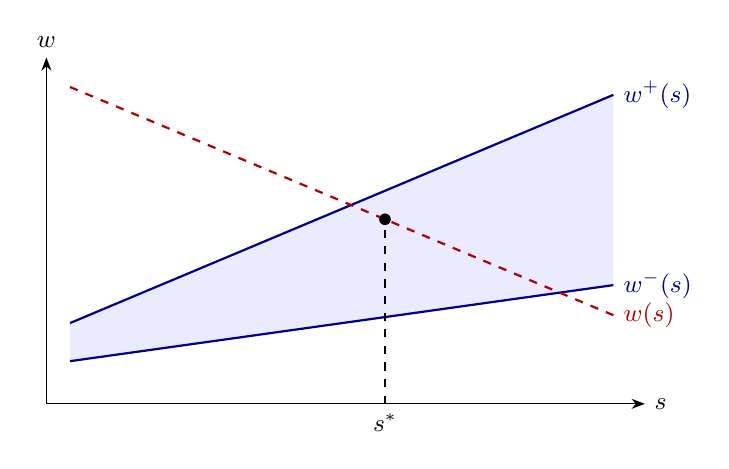
\begin{tikzpicture}[line width=0.4pt]
  \draw[-{Stealth}] (0,0) -- (7.6,0) node[right,font=\small] {$s$};
  \draw[-{Stealth}] (0,0) -- (0,4.4) node[above,font=\small] {$w$};
  \fill[blue!8]
    plot[domain=0.3:7.2] (\x,{0.5+0.14*\x})
    -- plot[domain=7.2:0.3] (\x,{0.9+0.42*\x}) -- cycle;
  \draw[blue!55!black,thick,domain=0.3:7.2] plot (\x,{0.5+0.14*\x})
    node[right,font=\small] {$w^-(s)$};
  \draw[blue!55!black,thick,domain=0.3:7.2] plot (\x,{0.9+0.42*\x})
    node[right,font=\small] {$w^+(s)$};
  \draw[red!70!black,thick,dashed,domain=0.3:7.2] plot (\x,{4.15-0.42*\x})
    node[right,font=\small] {$w(s)$};
  \fill (4.3,{4.15-0.42*4.3}) circle (2.1pt);
  \draw[dashed] (4.3,0) node[below,font=\small] {$s^*$} -- (4.3,{4.15-0.42*4.3});
\end{tikzpicture}
\caption{The sweep. The reachable band (shaded, endpoints $w^\pm$) rises gently as
the budget $s$ grows; the required height $w(s)$ for a fixed target $x$ descends
along the admissible budgets. If the band is wide, the descending line cannot skip
it: some admissible $s^*$ lands inside, and there $x$ is realized.}
\label{fig:sweep-friendly}
\end{figure}

\emph{The target starts above the band and ends below it.} At the small end: let
$s_{\min}$ be the smallest admissible $s \ge S_0$; then $w(s_{\min}) \ge
(x - \delta(S_0 + e))/e$, which for large $x$ exceeds $s_{\min}$, hence exceeds
$w^+(s_{\min})$ by \eqref{eq:wplus-le-s} --- explicitly, $x > (\delta + e)(S_0 + e)$
suffices. At the large end: enlarge $S_0$ once and for all so that $w^+(s) \ge \delta$ for
every $s \ge S_0$ (possible since $w^+(s) \ge q_s \to \infty$; this depends only on
the word, not on $x$). For the largest admissible $s$ with $w(s) \ge 0$, the next
admissible step would take $w$ negative, so $0 \le w(s) < \delta \le w^+(s)$: at
that budget the target sits at or below the band's top.

\emph{No skipping.} Suppose, for contradiction, that no admissible $s \ge S_0$ has
$w(s) \in [w^-(s),\ w^+(s)]$. The target descends (by $\delta$ per admissible
step) from above the band to below its top; since it never lands inside, there must
be two \emph{consecutive} admissible budgets $s'$ and $s' + e$ with
\[
  w(s') \;>\; w^+(s')
  \qquad\text{and}\qquad
  w(s' + e) \;<\; w^-(s' + e) :
\]
the leap over the band happens between them. First, $s'$ is large: from
$w(s'+e) \le w^-(s'+e) \le w^+(s'+e) \le s' + e$ (again \eqref{eq:wplus-le-s}),
\[
  \frac{x - \delta(s'+e)}{e} \;\le\; s' + e
  \quad\Longrightarrow\quad
  s' + e \;\ge\; \frac{x}{\delta + e} ,
\]
so $s' \ge S_0$ holds automatically once $x \ge (\delta + e)(S_0 + e)$ --- the same
threshold as before, so no new constraint. Now stack the inequalities. The target
drops by exactly $\delta$ across the leap, and the band's floor rises by at most
$e$:
\[
  w^+(s') \;<\; w(s') \;=\; w(s' + e) + \delta
          \;\le\; w^-(s' + e) - 1 + \delta
          \;\le\; w^-(s') + e - 1 + \delta .
\]
Hence
\[
  \mathrm{width}(s') \;=\; w^+(s') - w^-(s') \;\le\; \delta + e - 2 \;=\; \delta' - 2
  \;\le\; d_2 - 2 ,
\]
contradicting the hypothesis $\mathrm{width}(s') \ge d_2 - 1$. So some admissible
$s^* \ge S_0$ has $w(s^*) \in [w^-(s^*), w^+(s^*)]$; by
Lemma~\ref{lem:interval-friendly} the integer $w(s^*)$ is actually attained, and
$x = \delta s^* + e\,w(s^*) \in kA - k a_1$.
\end{proof}

Look where the alphabet bound was spent: the contradiction needed
$\mathrm{width} \ge \delta' - 1$, and the hypothesis supplies $d_2 - 1 \ge \delta' -
1$. A band exactly one narrower could be leapt over --- the sweep operates with no
room to spare, a first taste of how tight the corner $d_2 = k$ will be.

\subsection{Wide or balanced: the width dichotomy}

The sweep shifts the burden: we must now show the band is wide. Width comes from
\emph{irregularity} of the word $h$ --- if some stretches are $1$-rich and others
$1$-poor, configurations can exploit both. The cleanest measure uses just two
indices. For $\sigma \ge 0$ define the \emph{two-index width}
\[
  W_2(\sigma) \;:=\; \max\{\, q_i + q_j \,:\, i + j = \sigma,\ i,j \ge 0 \,\}
            \;-\; \min\{\, q_i + q_j \,:\, i + j = \sigma,\ i,j \ge 0 \,\} .
\]

\begin{lemma}[Width dichotomy]\label{lem:width-friendly}
\phantom{.}
\begin{enumerate}
\item[\textup{(a)}] Suppose $W_2(\sigma_0) \ge 2$ for some $\sigma_0$, and suppose
      $k$ is odd or $d_2 \le k - 1$. Then $\mathrm{width}(s) \ge d_2 - 1$ for all
      sufficiently large $s$ --- and the sweep applies.
\item[\textup{(b)}] If instead $W_2(\sigma) \le 1$ for \emph{every} $\sigma$, then
      the word $h$ is balanced.
\end{enumerate}
\end{lemma}

\begin{proof}
(a) The engine is additivity: if we split the $k$ indices of a configuration into
groups with prescribed subtotal sums, the extreme values over each group add. Fix a
pair $(i^-, j^-)$ attaining the minimum in $W_2(\sigma_0)$ and a pair $(i^+, j^+)$
attaining the maximum, so the max exceeds the min by $W_2(\sigma_0) \ge 2$.

\emph{$k$ odd.} Write $k = 2u + 1$. For any $s \ge u\,\sigma_0$, build
configurations from $u$ pairs, each summing to $\sigma_0$, plus one leftover index
$j := s - u\sigma_0 \ge 0$: choosing all $u$ pairs to be $(i^+, j^+)$ gives value
$u \cdot \max + q_j$, choosing $(i^-, j^-)$ gives $u \cdot \min + q_j$. Hence
\[
  \mathrm{width}(s) \;\ge\; u\,W_2(\sigma_0) \;\ge\; 2u \;=\; k - 1 \;\ge\; d_2 - 1 ,
\]
using $d_2 \le k$.

\emph{$k$ even, $d_2 \le k-1$.} Write $k = 2u$. For $s \ge (u-1)\sigma_0$, use
$u - 1$ prescribed pairs at $\sigma_0$ plus one \emph{free} pair with sum
$\tau := s - (u-1)\sigma_0 \ge 0$ (any split $\tau = i + j$): the prescribed pairs
alone already force
\[
  \mathrm{width}(s) \;\ge\; (u-1)\,W_2(\sigma_0) \;\ge\; 2u - 2 \;=\; k - 2 \;\ge\;
  d_2 - 1 .
\]

(b) Take two equal-length windows, from $i$ to $i'$ and from $j'$ to $j$ (so
$i' - i = j - j'$, i.e.\ $i + j = i' + j' =: \sigma$). Then
\[
  \big| (q_{i'} - q_i) - (q_j - q_{j'}) \big|
  \;=\; \big| (q_{i'} + q_{j'}) - (q_i + q_j) \big|
  \;\le\; W_2(\sigma) \;\le\; 1 ,
\]
which is precisely balancedness.
\end{proof}

Part (a)'s parity split is not laziness. When $k$ is even and $d_2 = k$, the
budget of $k$ indices is exactly wrong: $u$ full pairs use all $k$ indices and give
width $\ge k$ --- but only when $s$ has the right form --- while $u - 1$ pairs
guarantee only $k - 2 = d_2 - 2$, one short of what the sweep needs. This single
missing unit of width is a genuine boundary phenomenon, and
\S\ref{sec:sturmian-endgame} will close it with a separate argument
(Lemma~\ref{lem:boundary-friendly}) rather than a sharper pairing.

\emph{Where we stand.} If some $W_2(\sigma_0) \ge 2$ and ($k$ odd or $d_2 \le
k-1$): done, by (a) and the sweep. If every $W_2(\sigma) \le 1$: the word is
balanced, and the next section classifies it --- eventually periodic (done, by
\S\ref{sec:periodic}) or Sturmian (handled in \S\ref{sec:sturmian-endgame}). The
one remaining configuration, $k$ even with $d_2 = k$ and the word unbalanced, is
also settled in \S\ref{sec:sturmian-endgame}. The ledger stays honest.

\begin{checkpoint}
For the periodic word $h = 0011\,0011\cdots$ (which Example~\ref{ex:balanced-words}
showed is unbalanced), find a $\sigma_0$ with $W_2(\sigma_0) \ge 2$, and exhibit,
for $k = 3$, $s = 12$, two configurations whose values differ by at least $2$.
\end{checkpoint}

\begin{checkpoint}
$W_2$ uses exactly two indices while $\mathrm{width}$ uses $k$; compare them. Prove
that $\mathrm{width}(s) \ge W_2(\sigma)$ whenever $s \ge \sigma$ and $k \ge 2$ (pad
the two-index configurations with zeros --- $q_0 = 0$ costs nothing), and find a
word and an $s$ with $\mathrm{width}(s) > W_2(s)$.
\end{checkpoint}

\section{Balanced words: the Morse--Hedlund classification}\label{sec:sturmian-course}

The width dichotomy left us with the balanced words, and this section proves the
structure theorem that tames them: \emph{a balanced binary word is either eventually
periodic, or --- after discarding at most one initial stretch --- is ``mechanical'':
its counting function is $q_n = \lfloor n\alpha + \beta \rfloor$ for a fixed
irrational slope $\alpha$.} This is (one direction of) a celebrated 1940 theorem of
Morse and Hedlund. The proof below is elementary and self-contained: its only
imported ingredient is the completeness of the reals (through $\sup$), and the
section closes with the one approximation tool (Dirichlet, by pigeonhole) that the
endgame will need.

Throughout, $h$ is a balanced binary word with counting function $q$ ($q_0 = 0$).

\subsection{Step 1: a balanced word is nearly additive}

\begin{lemma}[Near-additivity]\label{lem:near-add}
For all $n, m \ge 0$:\quad $|\, q_{n+m} - q_n - q_m \,| \;\le\; 1$.
\end{lemma}

\begin{proof}
$q_{n+m} - q_n$ counts the $1$s in the window of length $m$ starting after position
$n$; $q_m$ counts them in the window of length $m$ at the very start. Balance bounds
the difference by $1$.
\end{proof}

Iterating pins down long-range behavior:

\begin{lemma}\label{lem:iterate}
For all $n \ge 0$, $t \ge 1$:\quad
$t\,q_n - (t-1) \;\le\; q_{tn} \;\le\; t\,q_n + (t-1)$.
\end{lemma}

\begin{proof}
Induct on $t$. Trivial at $t = 1$. If it holds at $t$, then by
Lemma~\ref{lem:near-add} (with the pair $tn, n$),
$q_{(t+1)n} \le q_{tn} + q_n + 1 \le (t+1)q_n + t$, and similarly from below.
\end{proof}

\subsection{Step 2: the slope}

\begin{lemma}[The slope exists]\label{lem:slope}
There is a real number $\alpha \in [0, 1]$ such that
\[
  |D_n| \;\le\; 1 \quad\text{for every } n \ge 0, \qquad\text{where } D_n := q_n -
  n\alpha .
\]
Moreover $q_n / n \to \alpha$.
\end{lemma}

\begin{proof}
The key inequality: for all $n, m \ge 1$,
\begin{equation}\label{eq:key-slope}
  m\,q_n - n\,q_m \;\le\; n + m - 2 .
\end{equation}
To see it, bound $q_{nm}$ twice by Lemma~\ref{lem:iterate}: viewing $nm$ as $m$
copies of $n$, $q_{nm} \ge m q_n - (m-1)$; viewing it as $n$ copies of $m$,
$q_{nm} \le n q_m + (n-1)$. Chaining the two gives \eqref{eq:key-slope}.

Dividing \eqref{eq:key-slope} by $nm$:
\[
  \frac{q_n - 1}{n} \;-\; \frac{q_m + 1}{m} \;=\;
  \frac{m q_n - n q_m - (n + m)}{nm} \;\le\; \frac{-2}{nm} \;<\; 0 .
\]
So \emph{every} number of the form $(q_n - 1)/n$ is below \emph{every} number of the
form $(q_m + 1)/m$. The set $\{(q_n - 1)/n : n \ge 1\}$ is therefore bounded above;
let
\[
  \alpha \;:=\; \sup_{n \ge 1} \frac{q_n - 1}{n} .
\]
By construction $(q_n - 1)/n \le \alpha$ for every $n$; and $\alpha \le
(q_m + 1)/m$ for every $m$, because $(q_m+1)/m$ is an upper bound of the set. The
two together read $q_n - 1 \le n\alpha \le q_n + 1$, i.e.\ $|D_n| \le 1$ (also at
$n = 0$, where $D_0 = 0$). Since $0 \le q_n \le n$, we get $(q_n - 1)/n < 1$ for
all $n$, so $\alpha \le 1$; and $\alpha \ge (q_n - 1)/n \ge -1/n$ for every $n$, so
$\alpha \ge 0$. Finally $|q_n/n - \alpha| = |D_n|/n \le 1/n \to 0$.
\end{proof}

The number $\alpha$ is the \emph{slope} of $h$: the limiting density of $1$s. The
inequality $|D_n| \le 1$ says the word tracks the line $y = \alpha x$ with error
never exceeding $1$ --- already a strong rigidity statement, extracted from balance
alone.

\subsection{Step 3: the discrepancy barely oscillates}

\begin{lemma}[Oscillation bound]\label{lem:osc}
For all $n, m \ge 0$:\quad $|D_n - D_m| \le 1$.
\end{lemma}

\begin{proof}
Say $m = n + \Delta$ with $\Delta \ge 1$. For $j \ge 0$ let
$W(j) := q_{j + \Delta} - q_j$ count the $1$s in the length-$\Delta$ window starting
after $j$; balance gives $|W(j) - W(n)| \le 1$ for every $j$. Sum $W$ over the $t$
consecutive disjoint windows starting at $0, \Delta, 2\Delta, \dots, (t-1)\Delta$;
the sum telescopes to $q_{t\Delta}$, and each summand lies within $1$ of $W(n)$:
\[
  t\,\big(W(n) - 1\big) \;\le\; q_{t\Delta} \;\le\; t\,\big(W(n) + 1\big) .
\]
Divide by $t\Delta$ and let $t \to \infty$: the middle tends to $\alpha$
(Lemma~\ref{lem:slope}), so by the limit facts of \S\ref{sec:words},
\[
  \frac{W(n) - 1}{\Delta} \;\le\; \alpha \;\le\; \frac{W(n) + 1}{\Delta} ,
  \qquad\text{i.e.}\qquad |W(n) - \Delta\alpha| \;\le\; 1 .
\]
And $D_{n+\Delta} - D_n = (q_{n+\Delta} - q_n) - \Delta\alpha = W(n) -
\Delta\alpha$.
\end{proof}

So all the discrepancies $D_0, D_1, D_2, \dots$ live in a band of height $1$ ---
they may drift within it, but no two ever differ by more than $1$. Everything below
flows from this single fact.

\subsection{Step 4: rational slope forces eventual periodicity}

\begin{proposition}\label{prop:rational-case}
If $\alpha$ is rational, $h$ is eventually periodic.
\end{proposition}

\begin{proof}
Write $\alpha = p/q$ in lowest terms ($q \ge 1$) and set
\[
  c_n \;:=\; q\,q_n - p\,n \;=\; q\,D_n ,
\]
an \emph{integer} with $|c_n| \le q$ (Lemma~\ref{lem:slope}). Let
$w_n := q_{n+q} - q_n$ (the $1$-count of the length-$q$ window after $n$), so that
\[
  c_{n+q} - c_n \;=\; q\,(w_n - p) .
\]
Balance confines the $w_n$ to two consecutive values $\{W, W+1\}$ (all length-$q$
windows agree to within one). We claim $p \in \{W, W{+}1\}$: if every
$w_n \ge p + 1$, then $c_{n+q} - c_n \ge q$ for every $n$, so following the indices
$n, n+q, n+2q, \dots$ the integer $c$ climbs by at least $q$ per step, exiting
$[-q, q]$ --- impossible; symmetrically, $w_n \le p - 1$ for all $n$ is impossible.
So either $w_n \in \{p, p+1\}$ for all $n$, or $w_n \in \{p-1, p\}$ for all $n$.

In the first case, $c_{n+q} - c_n \in \{0, q\}$: along each of the $q$ index classes
modulo $q$, the sequence $c$ is nondecreasing and bounded, hence eventually
constant; from some point on, no step of $+q$ ever occurs, i.e.\ $w_n = p$ for all
large $n$. The second case is the mirror image (nonincreasing), with the same
conclusion. So $q_{n+q} = q_n + p$ for all large $n$, and then
\[
  h_{n+q+1} \;=\; q_{n+q+1} - q_{n+q} \;=\; (q_{n+1} + p) - (q_n + p) \;=\; h_{n+1}
\]
for all large $n$: the word repeats with period $q$ from some point on.
\end{proof}

\subsection{Step 5: irrational slope forces a mechanical tail}

\begin{definition}[Mechanical word]\label{def:mechanical}
A binary word $h$ is \emph{mechanical} with slope $\alpha$ and intercept $\beta$ if
\[
  q_n \;=\; \lfloor n\alpha + \beta \rfloor \qquad \text{for every } n \ge 1 .
\]
Mechanical words with irrational slope are called \emph{Sturmian}.
\end{definition}

(A mechanical word is the ``digitized straight line'' of slope $\alpha$: its $n$-th
letter records whether the line $y = \alpha x + \beta$ crosses an integer height in
the $n$-th unit interval. Beatty walks and mechanical words are two costumes of the
same actor --- compare Definition~\ref{def:beatty-walk}.)

\begin{proposition}\label{prop:irrational-case}
If $\alpha$ is irrational, then there is an index $n_0 \ge 0$ such that the shifted
word $h'_j := h_{n_0 + j}$ is mechanical with slope $\alpha$ (and some intercept
$\beta'$).
\end{proposition}

\begin{proof}
Set $\beta := \sup_n D_n$, finite since $|D_n| \le 1$. By the oscillation bound,
every $D_n \ge \beta - 1$: for any $m$, $D_m - D_n \le 1$, and taking the supremum
over $m$ gives $\beta - D_n \le 1$.

When does the mechanical formula hold at $n$? Unwinding the floor's definition,
\[
  q_n = \lfloor n\alpha + \beta \rfloor
  \;\iff\; n\alpha + \beta - 1 < q_n \le n\alpha + \beta
  \;\iff\; \beta - 1 < D_n \le \beta .
\]
The upper half is the definition of $\beta$; the lower half holds at least weakly
($D_n \ge \beta - 1$), so the formula can fail only where $D_n = \beta - 1$ exactly
--- equivalently where $n\alpha + \beta = q_n + 1$ is an integer. If two distinct
indices $n_1 \ne n_2$ both had $n_i \alpha + \beta \in \ZZ$, subtracting would give
$(n_1 - n_2)\alpha \in \ZZ$, impossible for irrational $\alpha$. So there is at
most one exceptional index; call it $n_0$ (and set $n_0 := 0$ if there is none).

Discard everything through $n_0$: the word $h'_j := h_{n_0 + j}$ has counting
function $q'_j = q_{n_0 + j} - q_{n_0}$, and for every $j \ge 1$ the index
$n_0 + j$ is unexceptional, so
\[
  q'_j \;=\; \lfloor (n_0 + j)\alpha + \beta \rfloor - q_{n_0}
       \;=\; \lfloor j\alpha + (n_0\alpha + \beta - q_{n_0}) \rfloor
       \;=\; \lfloor j\alpha + \beta' \rfloor,
  \qquad \beta' := \beta - D_{n_0} ,
\]
where the middle equality moves the \emph{integer} $q_{n_0}$ through the floor
(Lemma~\ref{lem:floor-toolbox}(2)).
\end{proof}

Assembling Steps 4 and 5:

\begin{theorem}[Balanced classification]\label{thm:mh-friendly}
A balanced binary word is either eventually periodic, or agrees beyond some index
with a Sturmian word: a mechanical word of irrational slope $\alpha \in (0,1)$.
\end{theorem}

\begin{proof}
Steps 2--5; when $\alpha$ is irrational it lies in $(0,1)$, being in $[0,1]$ and not
equal to $0$ or $1$.
\end{proof}

For our purposes the theorem is a perfect fork: the periodic branch was closed in
\S\ref{sec:periodic}, so \emph{the only balanced words still standing are the
Sturmian tails}, with an explicit formula $q_n = \lfloor n\alpha + \beta \rfloor$ to
attack. The attack needs one lever: the ability to find indices $n$ where the
fractional part $\{n\alpha + \beta\}$ lands in any prescribed arc. That is a
statement about \emph{rotations of a circle}, and it closes this section.

\subsection{Rotations, and how to hit an arc on schedule}

For a real $x$ write $\{x\} := x - \lfloor x \rfloor \in [0, 1)$ for its
\emph{fractional part}. Picture the interval $[0,1)$ bent into a circle of
circumference $1$; the map $x \mapsto \{x + \alpha\}$ is rotation by $\alpha$. The
numbers $\{n\alpha + \beta\}$ are the successive positions of a point rotating by
$\alpha$ per tick. Write $\|x\|$ for the distance from $x$ to the nearest integer
--- the circle distance from $\{x\}$ to $0$.

\begin{lemma}[Dirichlet's approximation theorem]\label{lem:dirichlet}
For every real $\alpha$ and integer $Q \ge 1$ there are integers $n_0, m$ with
$1 \le n_0 \le Q$ and
\[
  |\, n_0 \alpha - m \,| \;<\; \frac{1}{Q} .
\]
\end{lemma}

\begin{proof}
Pigeonhole. The $Q + 1$ numbers $\{0 \cdot \alpha\}, \{1 \cdot \alpha\}, \dots,
\{Q\alpha\}$ all lie in $[0,1)$, which we cut into $Q$ boxes $[i/Q,\ (i+1)/Q)$.
Two of them share a box: $\{j\alpha\}$ and $\{j'\alpha\}$ with $j < j'$, differing
by less than $1/Q$. Set $n_0 := j' - j \in [1, Q]$; then $n_0\alpha =
(j'\alpha - \lfloor j'\alpha \rfloor) - (j\alpha - \lfloor j\alpha \rfloor) +
(\lfloor j'\alpha \rfloor - \lfloor j\alpha \rfloor) = \{j'\alpha\} - \{j\alpha\} +
m$ for the integer $m := \lfloor j'\alpha \rfloor - \lfloor j\alpha \rfloor$, and
$|n_0\alpha - m| = |\{j'\alpha\} - \{j\alpha\}| < 1/Q$.
\end{proof}

\begin{lemma}[Uniform hitting]\label{lem:hitting-friendly}
Let $\alpha \in (0,1)$ be irrational and $\beta \in \RR$. For every $\varepsilon >
0$ there is an integer $L = L(\alpha, \varepsilon)$ --- depending only on $\alpha$
and $\varepsilon$, \emph{not} on $\beta$ and not on the arc's position --- such that
for every arc $J \subseteq (0,1)$ of length $\ge \varepsilon$ and every $N \ge 0$,
some index $n \in \{N+1, \dots, N+L\}$ has $\{n\alpha + \beta\} \in J$.
\end{lemma}

\begin{proof}
An explicit \emph{circle walk}. Choose an integer $Q > 2/\varepsilon$ and apply
Dirichlet: there are $1 \le n_0 \le Q$ and $m$ with $\theta := |n_0\alpha - m| <
1/Q < \varepsilon/2$; and $\theta \ne 0$ since $\alpha$ is irrational. Advancing the
index by $n_0$ rotates the point $\{n\alpha + \beta\}$ by exactly $\theta$ around
the circle --- always in the same direction (the sign of $n_0\alpha - m$ is fixed).

Now fix $N$, and follow the $\lceil 1/\theta \rceil + 1$ indices
\[
  n_j \;:=\; N + (j+1)\,n_0 \qquad \big(j = 0, 1, \dots, \lceil 1/\theta \rceil\big),
\]
all lying in $\{N+1, \dots, N+L\}$ for
$L := n_0 \big( \lceil 1/\theta \rceil + 1 \big)$. The successive positions $x_j :=
\{n_j \alpha + \beta\}$ each step a fixed distance $\theta$ around the circle, in a
fixed direction, and over $\lceil 1/\theta \rceil$ steps the total distance walked
is at least $1$: the walk laps the whole circle. If none of the $x_j$ lay in the
arc $J$, then some single step would have to jump clean over $J$ --- but each step
has length $\theta < \varepsilon/2 < |J|$, too short to clear it. So some $x_j \in
J$.

Finally, audit the dependence: $Q$ came from $\varepsilon$; $n_0$, $m$, $\theta$
from $\alpha$ and $Q$; and $L = n_0(\lceil 1/\theta \rceil + 1) \le Q(\lceil
1/\theta\rceil + 1)$ from these. Neither $\beta$, nor $N$, nor where $J$ sits was
used --- only $|J| \ge \varepsilon$.
\end{proof}

The uniformity is the point: in the endgame the arc $J$ will \emph{move} as the
target changes, and we need a single window length $L$ serving every position. A
subtler equidistribution theorem would say more; this crude walking bound, powered
by one pigeonhole, says exactly enough.

\begin{checkpoint}
(a) For the periodic balanced word $001001\cdots$, compute $\alpha$ and check
$|D_n| \le 1$ and the conclusion of Step 4 directly.
(b) For $\alpha = \sqrt2 - 1$ and $Q = 5$, find the $n_0 \le 5$ and $\theta$
that Dirichlet's pigeonhole produces, and the resulting $L$ for $\varepsilon =
\tfrac15$.
\end{checkpoint}

\begin{checkpoint}
Where exactly did Step 5 use irrationality? (Two places. Find both, and check the
argument really does collapse for rational $\alpha$ --- as it must, since periodic
words are not mechanical-with-irrational-slope.)
\end{checkpoint}

\section{The Sturmian endgame}\label{sec:sturmian-endgame}

This section finishes the two-letter case: first the Sturmian walks (the hardest
single proof in this document --- take it slowly), then the boundary configuration
that the width dichotomy could not reach, then the assembled two-letter theorem.

\subsection{The Sturmian lemma}

We keep the two-letter coordinates of \S\ref{sec:widths} --- letters $\delta <
\delta' = \delta + e$ with $\gcd(\delta, e) = 1$ and $\delta' \le d_2 \le k$, binary
word $h$, counting function $q$ --- and now assume, after
Theorem~\ref{thm:mh-friendly} and a final tail-pass, that the word is Sturmian:
\[
  q_n \;=\; \lfloor n\alpha + \beta \rfloor \qquad (n \ge 1)
\]
for an irrational $\alpha \in (0,1)$ and some real $\beta$.

\begin{lemma}[Sturmian]\label{lem:sturmian-friendly}
In this situation $kA - k a_1$ contains every sufficiently large integer; in
particular $A$ is tail-covering with modulus $1$.
\end{lemma}

This is stronger than the sweep gave us --- \emph{all} large integers, no residue
class needed --- and it has to be, because Sturmian words are exactly the words for
which the band of \S\ref{sec:widths} is too narrow for the sweep. The proof replaces
``wide band'' with something better: \emph{exact control}. For a mechanical word the
value of a configuration is not merely trapped in a window; it can be steered onto a
precise target, because choosing indices means choosing points of an irrational
rotation, and the hitting lemma lets us place those points wherever we like.

\begin{proof}
Recall (Lemma~\ref{lem:kA-prefix} and \eqref{eq:two-letter-coords}) that it
suffices to realize each large integer $x$ as $x = \delta s + e\,w$ where $w$ is a
sum of $k$ counting-function values $q_{i_1} + \cdots + q_{i_k}$ with $i_t \ge 1$
and $i_1 + \cdots + i_k = s$. The proof has four movements.

\smallskip
\emph{Step 0: where the values live.} Write, for $n \ge 1$,
\[
  q_n \;=\; n\alpha + \beta - \{n\alpha + \beta\}
\]
(floor $=$ number minus fractional part). Summing over $k$ indices with total $s$:
\begin{equation}\label{eq:Xs}
  \sum_{t=1}^{k} q_{i_t} \;=\; X_s - \sum_{t=1}^{k} \{i_t \alpha + \beta\},
  \qquad X_s \;:=\; s\,\alpha + k\,\beta .
\end{equation}
Each fractional part lies in $[0,1)$, so the sum of $k$ of them lies in $[0, k)$:
every achievable value sits in the real window $(X_s - k,\ X_s]$ --- the two-letter
avatar of Part~II's window picture. But now we run the logic \emph{forward}: to
achieve a prescribed value $w$ at depth $\theta := X_s - w$ below the window's top,
it suffices to make the fractional parts sum to \emph{exactly} $\theta$.

\smallskip
\emph{Step 1: the tool.} Lemma~\ref{lem:hitting-friendly}: for any arc length
$\varepsilon > 0$ there is a window length $L(\alpha, \varepsilon)$ such that every
$L$ consecutive indices contain one whose rotation point $\{n\alpha + \beta\}$ lies
in any prescribed arc of length $\varepsilon$ --- uniformly in the arc's position.

\smallskip
\emph{Step 2: hitting any depth in the middle of the window.} Fix a margin $\eta
\in (0, \tfrac12)$, to be chosen in Step 3. \textbf{Claim:} there is a threshold
$S_0$ (depending on $\eta$, $\alpha$, $\beta$, $k$ only) such that for every $s \ge
S_0$ and every integer $w$ whose depth $\theta = X_s - w$ lies in $[\eta,\ k -
\eta]$, there are \emph{distinct} indices $i_1 < \cdots < i_k$ (all $\ge 1$, summing
to $s$) with
\[
  \sum_{t=1}^{k} \{ i_t \alpha + \beta \} \;=\; \theta \quad\text{exactly},
  \qquad\text{hence}\qquad \sum_{t=1}^{k} q_{i_t} = w .
\]

The mechanism: place the first $k-1$ points of the rotation in a narrow arc
positioned so their sum falls just below $\theta$, then let the forced last index
close the books --- with an integrality argument snapping the total onto $\theta$
exactly.

Set $\kappa := \eta/4$, and consider the open interval of candidate ``per-point
targets''
\[
  \mathcal{I} \;:=\; \big(\, \max(0,\ \theta - 1) + \kappa,\ \; \min(k-1,\ \theta)
  - \kappa \,\big) .
\]
Its length is at least $\eta/2$ whatever the regime of $\theta$: for $\eta \le
\theta \le 1$ it is $\theta - 2\kappa \ge \eta/2$; for $1 < \theta \le k-1$ it is
$1 - 2\kappa > \eta/2$; for $k - 1 < \theta \le k - \eta$ it is $(k - \theta) -
2\kappa \ge \eta/2$. Pick any $T^* \in \mathcal{I}$ and set the arc
\[
  J \;:=\; \Big( \frac{T^*}{k-1} - \frac{\kappa}{k-1},\ \frac{T^*}{k-1} +
  \frac{\kappa}{k-1} \Big) \;\subseteq\; (0,1),
\]
of length $\varepsilon_0 := 2\kappa/(k-1)$, and let $L := L(\alpha, \varepsilon_0)$
be its hitting constant. The arc's \emph{position} depends on $\theta$ (through
$T^*$), but its \emph{length} does not --- and the hitting lemma is uniform in
position, so this single $L$ serves every target and every $s$. (This is exactly
why we insisted on uniformity in \S\ref{sec:sturmian-course}.)

\emph{Choosing the free indices.} For $j = 1, \dots, k-1$, the hitting lemma finds
an index $i_j$ in the block $\{(j-1)L + 1, \dots, jL\}$ with
$\{i_j \alpha + \beta\} \in J$. Different blocks, so $i_1 < i_2 < \cdots <
i_{k-1}$, with
\begin{equation}\label{eq:free-bounds}
  i_j \le jL, \qquad \sum_{j=1}^{k-1} i_j \;\le\; L\,\frac{k(k-1)}{2}, \qquad
  i_{k-1} \le (k-1)L .
\end{equation}

\emph{The forced last index.} Set
\[
  S_0 \;:=\; 1 + L\,(k-1)\Big(\frac{k}{2} + 1\Big)
\]
(an integer: $(k-1)(k+2)/2$ has one even factor) and, for $s \ge S_0$, let
$i_k := s - (i_1 + \cdots + i_{k-1})$. By \eqref{eq:free-bounds},
\[
  i_k \;\ge\; S_0 - L\frac{k(k-1)}{2} \;=\; 1 + L(k-1)\Big(\frac k2 + 1 - \frac
  k2\Big) \;=\; 1 + (k-1)L \;>\; i_{k-1} ,
\]
so all $k$ indices are distinct and $\ge 1$, with total exactly $s$.

\emph{The snap.} Let $F := \sum_{j \le k-1} \{i_j\alpha + \beta\}$; since each term
lies in $J$,
\[
  F \;\in\; \big( T^* - \kappa,\ T^* + \kappa \big) \;\subseteq\;
  \big( \max(0, \theta - 1),\ \min(k-1, \theta) \big),
\]
the inclusion because $T^* \in \mathcal{I}$ keeps distance $> \kappa$ from both
endpoints. Add the last point: $\Theta := F + \{i_k \alpha + \beta\}$, with the
fractional part in $[0, 1)$, satisfies
\[
  \Theta \;>\; \max(0, \theta - 1) \;\ge\; \theta - 1
  \qquad\text{and}\qquad
  \Theta \;<\; \min(k-1, \theta) + 1 \;\le\; \theta + 1 .
\]
On the other hand, by \eqref{eq:Xs} applied to our indices,
\[
  \Theta \;=\; X_s - \sum_{t \le k} q_{i_t} ,
\]
and both $X_s - \theta = w$ and $\sum q_{i_t}$ are integers, so $\Theta$ differs
from $\theta$ by an integer. An integer-shift of $\theta$ lying strictly between
$\theta - 1$ and $\theta + 1$ must be $\theta$ itself: $\Theta = \theta$, and
$\sum_t q_{i_t} = X_s - \theta = w$. The Claim is proved.

\smallskip
\emph{Step 3: the ladder.} Now fix the margin
\[
  \eta \;:=\; \tfrac14 \min(\alpha,\ 1 - \alpha) \;\in\; (0, \tfrac18] ,
\]
and let $S_0$ be the resulting threshold. Let $x$ be a large integer. As in the
sweep, the budgets $s$ able to represent $x = \delta s + e w$ with integer $w$ form
one residue class modulo $e$ (the \emph{admissible} $s$), and for admissible $s$ we
set $w(s) := (x - \delta s)/e$ and measure the depth
\[
  \theta(s) \;:=\; X_s - w(s) \;=\; s\alpha + k\beta - \frac{x - \delta s}{e} .
\]
Per admissible step $s \mapsto s + e$, the value $X_s$ grows by $e\alpha$ and
$w(s)$ falls by $\delta$, so the depth climbs by exactly
\[
  \psi \;:=\; e\,\alpha + \delta \;>\; 0
\]
--- an arithmetic ladder. Step 2 accepts any depth in the strip $[\eta,\ k -
\eta]$, of height $k - 2\eta$. The ladder cannot step over the strip, because its
rung spacing is smaller:
\[
  \psi \;=\; \delta + e\alpha \;=\; \delta' - e(1 - \alpha) \;\le\; k - (1 -
  \alpha) \;<\; k - 2\eta ,
\]
using $\delta' \le k$, $e \ge 1$, and $2\eta \le \tfrac12(1-\alpha) < 1 - \alpha$.
Since $\theta(s)$ is very negative for small admissible $s$ (there $w(s) \approx
x/e$ dominates) and climbs unboundedly by steps $\psi < k - 2\eta$, some admissible
$s^*$ lands in the strip: $\theta(s^*) \in [\eta,\ k - \eta]$.

\emph{The thresholds, explicitly.} Multiplying the definition of $\theta$ by $e$
and rearranging: $s\psi = x + e\,\theta(s) - e k \beta$. So any $s^*$ with
$\theta(s^*) \in [0, k]$ satisfies
\[
  \frac{x - e k |\beta|}{\psi} \;\le\; s^* \;\le\; \frac{x + ek(1 + |\beta|)}{\psi}.
\]
Two requirements: (a) $s^* \ge S_0$, so Step 2 applies --- since $\psi \le \delta +
e = \delta' \le k$, the left bound gives this once $x \ge k S_0 + e k |\beta|$.
(b) $w(s^*) \ge 0$, i.e.\ $\delta s^* \le x$ --- by the right bound this holds once
$\delta\,(x + ek(1+|\beta|)) \le (\delta + e\alpha)\,x$, i.e.\ once $x \ge
\delta k (1 + |\beta|)/\alpha$ (here $\alpha > 0$ earns its keep). So for
\[
  x \;\ge\; X_0 \;:=\; 1 + \max\Big( k S_0 + ek|\beta| ,\ \ \frac{\delta k
  (1+|\beta|)}{\alpha} \Big),
\]
Step 2 realizes $w(s^*) \in W_{s^*}$ with legal indices, and
\[
  x \;=\; \delta\,s^* + e\,w(s^*) \;\in\; kA - k a_1 . \qedhere
\]
\end{proof}

\begin{bigidea}
For a Sturmian walk the window picture stops being an estimate and becomes an
equation: the depth of a value below the window's top \emph{equals} the sum of $k$
rotation points on the circle. The hitting lemma lets us place $k-1$ of those
points at will; integrality snaps the total onto the exact target; and the
irrationality of the slope makes the ladder's rung $\psi = \delta + e\alpha$
incommensurable-with-nothing --- just strictly shorter than the acceptance strip,
so no target escapes.
\end{bigidea}

\begin{example}[The Fibonacci walk, traced]\label{ex:fib-traced}
Take $k = 3$, letters $\{1, 2\}$ (so $\delta = e = 1$, every $s$ admissible), and
the Fibonacci gap word: $q_n = \lfloor n\alpha + \beta \rfloor$ with $\alpha =
(3 - \sqrt5)/2 \approx 0.382$ and $\beta = \alpha$. Then $\eta = \alpha/4 \approx
0.095$ and the ladder climbs by $\psi = 1 + \alpha \approx 1.382$ per step ---
comfortably below the strip height $3 - 2\eta \approx 2.81$. To represent
$x = 100$: $\theta(s) = (s + 3)\alpha - 100 + s$ climbs by $\psi$ and first enters
$[\eta,\ 3 - \eta]$ at $s^* = 72$, where $\theta(72) = 75\alpha - 28 \approx
0.647$. So $w = w(72) = 100 - 72 = 28$, and Step 2 must find three distinct indices
with $i_1 + i_2 + i_3 = 72$ and $q_{i_1} + q_{i_2} + q_{i_3} = 28$ --- three
rotation points summing to depth $0.647$. (One valid triple: $i = (10, 26, 36)$,
whose counting values are $4 + 10 + 14 = 28$ --- check them against $q_n = \lfloor
(n+1)\alpha \rfloor$.) Then $100 = 1 \cdot 72 + 1 \cdot 28 \in 3A - 3a_1$.
\end{example}

\subsection{The boundary: \texorpdfstring{$k$}{k} even, \texorpdfstring{$d_2 = k$}{d2 = k}}

One configuration escaped the width dichotomy: $k$ even at the exact boundary $d_2
= k$, where the pairing argument came up one unit of width short. The rescue is a
lemma that squeezes width out of \emph{unbalancedness itself}, with a beautiful
detour through palindromes.

First, a two-line classic:

\begin{lemma}[Border--period duality]\label{lem:border-period}
Let $u$ be a finite word of length $\tau$ with a \emph{border} of length $\ell$:
its prefix of length $\ell$ equals its suffix of length $\ell$. Then $u$ has
\emph{period} $\tau - \ell$: $u_i = u_{i + \tau - \ell}$ for all $1 \le i \le \ell$.
\end{lemma}

\begin{proof}
The border condition says $u_i = u_{(\tau - \ell) + i}$ for $1 \le i \le \ell$ ---
which \emph{is} the period condition, re-read.
\end{proof}

\begin{lemma}[Boundary width]\label{lem:boundary-friendly}
Let $k \ge 4$ be even. Suppose the binary word $h$ uses both letters infinitely
often, is not eventually periodic, and has the property that \emph{every} tail of
$h$ is unbalanced. Then $\mathrm{width}(s) \ge k - 1$ for all sufficiently large
$s$.
\end{lemma}

\begin{proof}
\emph{First, unbalancedness of every tail yields two-index width $\ge 2$
infinitely often.} Suppose instead $W_2(\sigma) \le 1$ for all $\sigma \ge
\sigma^*$. Take any two equal-length windows of the tail of $h$ beyond position
$\sigma^*$, say from $i$ to $i'$ and from $j'$ to $j$; then $\sigma := i + j =
i' + j' \ge \sigma^*$, and exactly as in
Lemma~\ref{lem:width-friendly}(b), $W_2(\sigma) \le 1$ bounds the difference of
their $1$-counts by $1$. So that tail would be balanced --- contradiction. Hence
$W_2(\sigma) \ge 2$ for infinitely many $\sigma$; fix two such, $\sigma_0 <
\sigma_1$, and set $\Delta := \sigma_1 - \sigma_0 \ge 1$.

\emph{Second, suppose the width bound fails at some large $s$:} $\mathrm{width}(s)
\le k - 2$. Play the two-family game of Lemma~\ref{lem:width-friendly}(a), but with
a twist. Family one: $k/2 - 1$ extremal pairs at $\sigma_0$ plus a free pair at
$\tau := s - (k/2 - 1)\sigma_0$; it forces $\mathrm{width}(s) \ge (k - 2) +
W_2(\tau)$, so $W_2(\tau) = 0$. Family two ($k \ge 4$ makes room): $k/2 - 2$ pairs
at $\sigma_0$, one pair at $\sigma_1$, and a free pair at $\tau - \Delta$; it
forces $W_2(\tau - \Delta) = 0$ likewise.

\emph{Third, zero two-index width means palindrome.} $W_2(\tau) = 0$ says $q_i +
q_{\tau - i}$ is constant over $0 \le i \le \tau$; differencing consecutive $i$
gives $h_{i+1} = h_{\tau - i}$ for $0 \le i \le \tau - 1$ --- the prefix
$h[1..\tau]$ reads the same forwards and backwards. So both $h[1..\tau]$ and
$h[1..\tau - \Delta]$ are palindromes. A palindromic prefix of a palindrome is also
its suffix (reverse the whole word: it is unchanged, and the prefix's mirror image
--- itself --- appears at the end). So $h[1..\tau - \Delta]$ is a border of
$h[1..\tau]$, and by Lemma~\ref{lem:border-period}, $h[1..\tau]$ has period
$\Delta$.

\emph{Finally, infinitely many failures would force global periodicity.} If
$\mathrm{width}(s) \le k-2$ for infinitely many $s$, then --- $\Delta$ being fixed
while $\tau = \tau(s) \to \infty$ --- we obtain arbitrarily long prefixes of $h$
with the \emph{same} period $\Delta$. Any fixed position $n$ is eventually covered
with room to spare, so $h_n = h_{n + \Delta}$ for every $n$: the whole word is
periodic, contradicting the hypothesis. Hence $\mathrm{width}(s) \ge k - 1$ for all
large $s$.
\end{proof}

\begin{proposition}[Boundary routing]\label{prop:boundary-friendly}
Let $k$ be even, $d_2 = k$, and let $A$ have two-letter tail alphabet (the standing
setup of \S\ref{sec:widths}). Then $A$ is tail-covering.
\end{proposition}

\begin{proof}
Route by the first case that applies; each closes the matter. If the gap word is
eventually periodic: Lemma~\ref{lem:periodic-friendly}. Otherwise, if \emph{some}
tail of the gap word is balanced: pass to that tail (Lemma~\ref{lem:tail-friendly})
and classify it (Theorem~\ref{thm:mh-friendly}) --- eventually periodic
(Lemma~\ref{lem:periodic-friendly} again) or Sturmian on a further tail
(Lemma~\ref{lem:sturmian-friendly}); note neither route used any width argument.
Otherwise \emph{every} tail is unbalanced and the word is not eventually periodic
(and $k \ge 4$, being even and $\ge 3$): Lemma~\ref{lem:boundary-friendly} gives
$\mathrm{width}(s) \ge k - 1 = d_2 - 1$ for large $s$, and the sweep
(Lemma~\ref{lem:sweep-friendly}) finishes.
\end{proof}

\subsection{The two-letter theorem}

\begin{theorem}[Two letters]\label{thm:twoletter-friendly}
Let $k \ge 3$ and $d_2 \le k$. Every $(d_1,d_2)$-sequence whose tail alphabet has
at most two letters is tail-covering.
\end{theorem}

\begin{proof}
One letter: Lemma~\ref{lem:oneletter-friendly}. Two letters: rescale to
$\gcd = 1$ (Lemma~\ref{lem:rescale-friendly}). If $k$ is even and $d_2 = k$:
Proposition~\ref{prop:boundary-friendly}. Otherwise $k$ is odd or $d_2 \le k - 1$,
and we consult the two-index widths: if $W_2(\sigma_0) \ge 2$ for some $\sigma_0$,
then Lemma~\ref{lem:width-friendly}(a) plus the sweep
(Lemma~\ref{lem:sweep-friendly}) conclude; if $W_2(\sigma) \le 1$ for all
$\sigma$, the word is balanced (Lemma~\ref{lem:width-friendly}(b)), hence
eventually periodic (Lemma~\ref{lem:periodic-friendly}) or Sturmian on a tail
(Theorem~\ref{thm:mh-friendly}, then Lemma~\ref{lem:sturmian-friendly}). Every
branch ends in tail-covering.
\end{proof}

\begin{checkpoint}
In Example~\ref{ex:fib-traced}, verify the claimed triple: generate the Fibonacci
word ($0 \mapsto 01$, $1 \mapsto 0$, starting from $0$), compute $q_{10}, q_{25},
q_{37}$, and check the two equations. Then find a different valid triple for the
same $x = 100$.
\end{checkpoint}

\begin{checkpoint}
Why can the Sturmian lemma not simply reuse the sweep? Locate the precise failure:
show that for a Sturmian word, $\mathrm{width}(s) \le$ some bound that falls short
of $d_2 - 1$ in the critical case $\delta' = d_2$. (Hint: Step 0 traps $W_s$ in a
real window of length $k$; how many integers can it contain, and what does
balancedness do to the endpoints?)
\end{checkpoint}

\section{Three or more letters: the slot lemma}\label{sec:slot}

One case of the battle plan remains: tail alphabets with three or more letters. The
band-and-sweep machinery does not survive the trip --- with three letters, a single
move between configurations changes the value by a \emph{difference of letters},
which can exceed $1$, so the reachable set $W_s$ can have holes and
Lemma~\ref{lem:interval-friendly} fails. Instead of repairing the band we change
weapons entirely: a small combinatorial gadget --- the \emph{slot lemma} --- that
spends the $k$ summands like a budget, and whose exact price is the finite theorem
of Part~IV.

\subsection{Subset sums of multisets}

\begin{definition}\label{def:msum}
A \emph{multiset} $S$ drawn from a set $G$ is a collection of elements of $G$ with
repetitions allowed ($|S|$ counts repetitions). Its \emph{subset sums} are
\[
  \ssum(S) \;:=\; \Big\{ \sum_{x \in T} x \;:\; T \text{ a sub-multiset of } S
  \Big\}
\]
(including the empty sum $0$). For a finite set $G$ of positive integers with $M :=
\max G$, define
\[
  m(G) \;:=\; \min\big\{\, |S| \;:\; S \text{ a multiset drawn from } G \text{
  whose subset sums contain $M$ consecutive integers} \,\big\} .
\]
\end{definition}

\begin{example}\label{ex:msum}
$G = \{3, 4, 5\}$, $S = \{3, 3, 4, 5\}$: the subset sums are
$\{0, 3, 4, 5, 6, 7, 8, 9, 10, 11, 12, 15\}$, which contain the run $3, 4, \dots,
12$ --- ten consecutive integers, amply covering $M = 5$. So $m(\{3,4,5\}) \le 4$.
(Part~IV will show $4$ is optimal here.)
\end{example}

Part~IV is devoted to proving:

\begin{quote}
\textbf{The bounded subset-sum covering lemma (SHARP).} \emph{Every finite set $G$
of at least three positive integers with $\gcd(G) = 1$ and $\max(G) = M$ has}
$m(G) \le M - 1$.
\end{quote}

For now we take it on credit and show exactly how the non-existence proof spends
it.

\subsection{The slot lemma}

\begin{lemma}[Slot lemma]\label{lem:slot-friendly}
Let $A$ have tail alphabet $\Ginf$ with $|\Ginf| \ge 3$ and $\gcd(\Ginf) = 1$
(after rescaling), and put $M := \max \Ginf \le d_2$. If $k - 1 \ge m(\Ginf)$, then
$A$ is tail-covering.
\end{lemma}

\begin{proof}
Pass to the tail (Lemma~\ref{lem:tail-friendly}): all gaps lie in $\Ginf$, all
letters recur infinitely often, and we work with prefix sums via
Lemma~\ref{lem:kA-prefix}. Let $S$ be a multiset realizing $m(\Ginf) =: m \le k-1$:
$|S| = m$, drawn from $\Ginf$, with
\[
  \ssum(S) \;\supseteq\; \{c,\ c+1,\ \dots,\ c + M - 1\}
\]
for some $c$. Enumerate $S$ as $\delta_1, \dots, \delta_m$ (values in $\Ginf$,
possibly repeating).

\emph{The fine slots.} Because each letter of $\Ginf$ occurs infinitely often in
the gap word, we can choose $m$ \emph{distinct} positions $n_1 < n_2 < \cdots <
n_m$ (all beyond the tail start) with
\[
  g_{n_t} = \delta_t \qquad (t = 1, \dots, m) .
\]
Summand $t$ of our $k$-fold sum will be confined to two adjacent choices: index
$n_t - 1$ (``off''), contributing the prefix sum $p_{n_t - 1}$, or index $n_t$
(``on''), contributing $p_{n_t} = p_{n_t - 1} + \delta_t$. Toggling slot $t$ from
off to on adds exactly $\delta_t$. Over all $2^m$ on/off patterns, the $m$ slots
jointly contribute
\[
  \Big( \sum_{t=1}^m p_{n_t - 1} \Big) + \ssum(S)
  \;\supseteq\; \mathrm{base}_0 + [\,c,\ c + M - 1\,],
  \qquad \mathrm{base}_0 := \sum_t p_{n_t - 1} :
\]
a full block of $M$ consecutive achievable offsets --- this is where the multiset's
covering run is cashed in.

\emph{The parked summands.} We have used $m$ of our $k$ summands. Park the next
$k - 1 - m$ at any fixed tail index (repetition of indices is legal in the
sumset), folding their fixed contribution into the base:
$\mathrm{base} := \mathrm{base}_0 + (\text{parked total})$. Now $k - 1$ summands
realize every value of $\mathrm{base} + [c,\ c + M - 1]$.

\emph{The coarse dial.} The final summand is an index $n$ of our choosing,
contributing $p_n$. In the tail, consecutive prefix sums differ by a gap
$g_{n+1} \in \Ginf \subseteq [1, M]$, so $n \mapsto p_n$ is strictly increasing
with steps of size at most $M$, tending to infinity: a coarse dial that ascends
forever but can jump by as much as $M$ at a time.

\emph{The first-crossing argument.} Fix a large target $x$ and let
\[
  \phi(n) \;:=\; x - \mathrm{base} - p_n ,
\]
which decreases strictly in $n$, in steps of at most $M$, from a starting value
$\phi(T) > c + M - 1$ (true once $x$ is large, the base and $T$ being fixed) down
toward $-\infty$. Let $n^*$ be the \emph{first} index past $T$ with $\phi(n^*) \le
c + M - 1$. By firstness, $\phi(n^* - 1) > c + M - 1$; and one step drops $\phi$ by
at most $M$, so
\[
  \phi(n^*) \;>\; (c + M - 1) - M \;=\; c - 1, \qquad\text{i.e.}\qquad \phi(n^*)
  \;\ge\; c .
\]
So $\phi(n^*)$ lands \emph{inside} the achievable block $[c,\ c+M-1]$: some on/off
pattern realizes the offset $\phi(n^*)$, and then
\[
  x \;=\; \mathrm{base} + \phi(n^*) + p_{n^*}
\]
exhibits $x$ as a sum of $k$ prefix sums --- $m$ slots, $k-1-m$ parked, one dial.
(The dial index may coincide with a slot or parked index; harmless, repetitions
are allowed.) Hence $kA - k a_1$ contains every large integer, and $A$ is
tail-covering (with the factor $g$ restored by Lemma~\ref{lem:rescale-friendly} if
rescaling was applied).
\end{proof}

Watch the accounting at the binding corner. The dial can step by $M$, so the
achievable block must be at least $M$ long --- a run of $M - 1$ consecutive offsets
would let the dial leap clean over it. The block costs $m(\Ginf)$ summands, the
dial costs one, and only $k$ are available:
\[
  m(\Ginf) \;\le\; k - 1 .
\]
When the Adversary's walk uses the largest legal gap infinitely often and the
parameters sit at the corner $k = d_2 = M$, this requirement becomes exactly
\[
  m(\Ginf) \;\le\; M - 1
\]
--- SHARP, with nothing to spare. The whole weight of the corner case rests on
that finite statement, which is why Part~IV exists. Away from the corner there is
slack: $m(\Ginf) \le M - 1 \le d_2 - 1 \le k - 1$ holds a fortiori.

For perspective --- not needed below --- a much cruder bound is easy to prove and
shows the mechanism in miniature:

\begin{lemma}[Base grid]\label{lem:basegrid}
Let $G$ have $|G| \ge 3$, $\gcd(G) = 1$, $a := \min G$, $M := \max G$, and suppose
some $c \in G$ has $\gcd(a, c) = 1$. Then $m(G) \le a + M - 1 \le 2M - 3$.
\end{lemma}

\begin{proof}
Take $a - 1$ copies of $c$ and $p := \lceil ((a-1)c + M - 1)/a \rceil$ copies of
$a$. For any $n \in [(a-1)c,\ pa]$: the residues $0, c, 2c, \dots, (a-1)c$ modulo
$a$ are pairwise distinct (as $\gcd(a,c)=1$), so a unique $i \in [0, a-1]$ has
$ic \equiv n \pmod a$; then $ic \le (a-1)c \le n$, and $(n - ic)/a$ is an integer
in $[0, p]$, so $n = ic + a \cdot \frac{n-ic}{a}$ is a subset sum. The interval
has length $pa - (a-1)c + 1 \ge M$ by the choice of $p$. The size: $c \le M$ gives
$p \le \lceil ((a-1)M + M - 1)/a \rceil = \lceil (aM-1)/a \rceil = M$, so
$(a-1) + p \le a + M - 1$; and $|G| \ge 3$ squeezes $a \le M - 2$.
\end{proof}

The gap between $2M - 3$ and SHARP's $M - 1$ is the gap between an evening's
exercise and Part~IV; note also the extra hypothesis, which genuinely can fail
($G = \{6, 10, 15\}$ has $\gcd 1$ but no element coprime to $6$).

\subsection{The non-existence half, assembled (modulo SHARP)}

\begin{proposition}[Goal of Part III]\label{prop:goal}
Assume SHARP. Then every $(d_1,d_2)$-sequence with $d_2 \le k$ and $k \ge 3$ is
tail-covering.
\end{proposition}

\begin{proof}
Pass to the tail; rescale so $\gcd(\Ginf) = 1$ (Lemmas~\ref{lem:tail-friendly},
\ref{lem:rescale-friendly}). If $|\Ginf| \le 2$:
Theorem~\ref{thm:twoletter-friendly}. If $|\Ginf| \ge 3$: SHARP applies to
$\Ginf$ (three or more elements, $\gcd 1$) and gives $m(\Ginf) \le \max(\Ginf) - 1
\le d_2 - 1 \le k - 1$, so the slot lemma (Lemma~\ref{lem:slot-friendly})
concludes.
\end{proof}

Combined with the certificate (Lemma~\ref{lem:cert-friendly}), this proves the
strong non-existence half of Theorem~\ref{thm:main-friendly} --- \emph{modulo
SHARP}. The debt is now fully explicit, and Part~IV pays it.

\begin{checkpoint}
(a) Show $m(\{1, 2, 3\}) \le 2$ and $m(\{2, 3, 4\}) \le 3$, with explicit
multisets. (b) Trace the slot lemma concretely: $k = 4$, $d_2 = 4$, $\Ginf =
\{2, 3, 4\}$ (so $M = 4$), gap word cycling $2, 3, 4, 2, 3, 4, \dots$ --- pick the multiset from (a), choose slot positions inside the first two
periods, and find the dial index and slot pattern realizing $x = 57$ (with $a_1$
of your choosing).
\end{checkpoint}

\begin{checkpoint}
The parked summands were placed at one fixed index. Would the proof survive
parking them at index $0$ (contributing $p_0 = 0$)? And why does the argument
insist the block have length $M$ rather than $M - 1$ --- exhibit a concrete
failure: a dial whose steps are all $M$ leaping over a block of length $M-1$.
\end{checkpoint}

%======================================================================
\part{The subset-sum lemma}
%======================================================================

\section{The subset-sum lemma: statement, sharpness, and the map}\label{sec:sharp-intro}

Part~IV is a self-contained piece of finite mathematics. It never mentions walks,
sumsets of sequences, or lacunarity; it proves exactly the statement that Part~III
left as a debt. Recall $m(G)$ from Definition~\ref{def:msum}: the smallest size of
a multiset drawn from $G$ whose subset sums contain $\max(G)$ consecutive integers.

\begin{theorem}[Bounded subset-sum covering --- ``SHARP'']\label{thm:sharp-friendly}
Every finite set $G$ of positive integers with $|G| \ge 3$, $\gcd(G) = 1$ and
$\max(G) = M$ satisfies
\[
  m(G) \;\le\; M - 1 .
\]
\end{theorem}

Before proving it (\S\S\ref{sec:sharp-machinery}--\ref{sec:sharp-assembly}), let us
be precise about what the bound claims, and check that neither hypothesis nor
constant can be weakened.

\subsection{First moves, and sharpness}

\emph{If $1 \in G$}, take $M - 1$ copies of $1$: the subset sums are $0, 1, \dots,
M-1$ --- exactly $M$ consecutive integers at budget $M-1$. So assume from now on
$a := \min G \ge 2$.

\emph{The constant cannot be improved to $M - 2$.} Take $G = \{3,4,5\}$, so $M =
5$. Example~\ref{ex:msum} showed $m(G) \le 4$ via $\{3,3,4,5\}$; we claim no
multiset of size $\le 3$ works, so $m(\{3,4,5\}) = 4 = M - 1$ exactly. This is a
finite check --- there are $3$ multisets of size one, $6$ of size two, and $10$ of
size three --- and the size-three table settles it (smaller multisets have fewer
sums and do no better):

\begin{center}\small
\begin{tabular}{@{}lll@{}}
\toprule
Multiset & Subset sums & Longest run \\
\midrule
$\{3,3,3\}$ & $0,3,6,9$ & $1$ \\
$\{3,3,4\}$ & $0,3,4,6,7,10$ & $2$ \\
$\{3,3,5\}$ & $0,3,5,6,8,11$ & $2$ \\
$\{3,4,4\}$ & $0,3,4,7,8,11$ & $2$ \\
$\{3,4,5\}$ & $0,3,4,5,7,8,9,12$ & $3$ \\
$\{3,5,5\}$ & $0,3,5,8,10,13$ & $1$ \\
$\{4,4,4\}$ & $0,4,8,12$ & $1$ \\
$\{4,4,5\}$ & $0,4,5,8,9,13$ & $2$ \\
$\{4,5,5\}$ & $0,4,5,9,10,14$ & $2$ \\
$\{5,5,5\}$ & $0,5,10,15$ & $1$ \\
\bottomrule
\end{tabular}
\end{center}

The best run of consecutive integers achievable with three elements is $3$,
short of the required $M = 5$.

\emph{The hypothesis $|G| \ge 3$ cannot be dropped.} Take $G = \{2, 3\}$: $\gcd =
1$, $M = 3$, and the target would be $m(G) \le 2$. The five nonempty multisets of
size $\le 2$ have subset sums
\[
  \{0,2\},\quad \{0,3\},\quad \{0,2,4\},\quad \{0,2,3,5\},\quad \{0,3,6\} ,
\]
and none contains $3$ consecutive integers. So two-element sets genuinely need
more room; three elements is where the uniform budget $M-1$ becomes available.

Finally, a caution about what SHARP does \emph{not} say: it is not a formula for
$m(G)$, which is usually far smaller than $M-1$ (for $G = \{1, 2, M\}$ it is
tiny --- see the checkpoint). It is a \emph{uniform budget},
tuned to be exactly what the slot lemma's corner $k = d_2 = M$ can afford ---
recall \S\ref{sec:slot}: one dial summand plus at most $M - 1$ slot summands is all
that $k = M$ pays for.

\begin{checkpoint}
(a) Compute $m(\{1, 2, M\})$ for general $M \ge 3$.
(b) A multiset of size $s$ has at most $2^s$ subset sums, and $M$ consecutive
integers are $M$ distinct sums; deduce the elementary lower bound $m(G) \ge \log_2
M$. Then find a three-element family of sets $G$ (one for each large $M$) whose
$m(G)$ is genuinely logarithmic-ish in $M$... or convince yourself that with only
three generators this is impossible, and explain which structural feature of $G$
controls how far below $M - 1$ the truth sits.
\end{checkpoint}

\subsection{The shape of the proof}\label{sec:sharp-shape}

The whole of Part~IV runs on a single covering mechanism, previewed here and built
in \S\ref{sec:sharp-machinery}. To cover $M$ consecutive integers with copies of
elements of $G$:

\begin{enumerate}
\item \emph{Cover the residues.} Using a bounded number of copies of the two
      largest generators, hit every residue class modulo $a$ (the smallest
      generator) at least once --- a \emph{box} of representatives.
\item \emph{Slide and stack.} Add $0, 1, 2, \dots, x$ copies of $a$: each
      representative slides up an arithmetic progression of step $a$, and the
      progressions interleave into a solid run once every class is represented and
      the run is long enough.
\end{enumerate}

The cost accounting --- how many copies of $a$ suffice, and whether the total stays
under $M - 1$ --- is the \emph{budget}, and the entire difficulty of Part~IV is
that near the corner the budget has no slack at all.

The proof organizes as follows.
\begin{itemize}
\item \S\ref{sec:sharp-machinery}: the covering machinery --- a two-generator
      interval lemma, the frame lemma (the slide-and-stack step made exact), the
      staircase (a refined multi-level version), and the $\lambda$-lift (a way to
      certify infinitely many triples with one finite check).
\item \S\ref{sec:sharp-reduction}: reduction of the general statement to
      \emph{hard-core triples} $\{a, b, M\}$ with $\gcd(a,b) = 1$ and $b$ close to
      $M$ (precisely $1 \le M - b \le a - 2$).
\item \S\S\ref{sec:caseDL}--\ref{sec:caseB-friendly}: the hard core is carved by
      simple arithmetic invariants into six branches --- D, P, L, E, T, B ---
      four closed by explicit formulas valid across their whole range, two (T and
      B) closed by formulas \emph{plus} a finite list of exceptional triples,
      each carrying a small computer-verified certificate. \S\ref{sec:computer}
      explains exactly what was computed and how it is checked.
\item \S\ref{sec:sharp-assembly}: assembly, exhaustiveness of the six branches,
      and the sharpness proposition.
\end{itemize}

The six-way split is by two divisibility questions and two size questions,
routed in order (evaluate top to bottom, take the first that applies):

\begin{center}\small
\begin{tabular}{@{}llll@{}}
\toprule
Branch & Condition & Mechanism & Closure \\
\midrule
D & $a \mid M$ & $b$ spans the residues alone & formula \\
P & $a \mid b + M$ & $(b,M)$ pairs as residue-neutral movers & formula \\
L & $e = h$ (equal spacings) & staircase, extended form & formula \\
E & $a \ge 12$ and $\mu \ge 12$ & the $\eta$-box & formula \\
T & $\mu \le 11$ & staircase lines; $172$ exceptions & formula $+$ table \\
B & $a \le 11$, $\mu \ge 12$ & $178$ base certificates, lifted & table $+$ lift \\
\bottomrule
\end{tabular}
\end{center}

\noindent(The symbols $e, h, \mu$ are set up in \S\ref{sec:sharp-machinery}; think
``$\mu$ small'' $=$ the generators are crowded near $M$, ``$a$ small'' $=$ the
smallest generator is tiny.)

\section{Machinery: grids, frames, staircases, and the lift}\label{sec:sharp-machinery}

Everything in Part~IV covers runs of consecutive integers by the same two-phase
mechanism sketched in \S\ref{sec:sharp-shape}. This section builds it once, with
exact constants, so the case sections can spend their attention on budgets.

\subsection{The two-generator grid}

How much of the number line do two coprime generators cover, using boundedly many
copies of each? The classic ``postage stamp'' fact --- with stamps of two coprime
denominations $\alpha, \beta$ and unlimited copies, every amount from
$(\alpha-1)(\beta-1)$ on is payable --- has the following bounded-copies version.

\begin{lemma}[Two-generator interval]\label{lem:twogen-friendly}
Let $\alpha < \beta$ be coprime positive integers, and let $x \ge \beta - 1$ and
$y \ge \alpha - 1$ be integers. Then, with $C := (\alpha - 1)(\beta - 1)$,
\[
  \{\, i\alpha + j\beta \;:\; 0 \le i \le x,\ 0 \le j \le y \,\}
  \;\supseteq\; [\,C,\ \; \alpha x + \beta y - C\,] .
\]
\end{lemma}

Note the symmetry of the conclusion: the grid covers everything except a margin of
$C$ at each end of its full span $[0,\ \alpha x + \beta y]$.

\begin{proof}
\emph{Case $\alpha = 1$.} Here $C = 0$. For $n \in [0,\ x + \beta y]$ put $j :=
\min(y,\ \lfloor n/\beta \rfloor)$. If $j = \lfloor n/\beta \rfloor$ then $n -
j\beta$ is the remainder, in $[0, \beta - 1] \subseteq [0, x]$; if instead $j = y$
then $n - y\beta \le x$ directly. Either way $i := n - j\beta \in [0, x]$.

\emph{Case $\alpha \ge 2$, base $y = \alpha - 1$.} Let $n \in [\,C,\ \alpha x +
\beta(\alpha-1) - C\,]$. Since $\gcd(\alpha, \beta) = 1$, the multiples $0, \beta,
2\beta, \dots, (\alpha-1)\beta$ hit all residues modulo $\alpha$; choose the unique
$j \in [0, \alpha - 1]$ with $j\beta \equiv n \pmod \alpha$. Then $n - j\beta$ is
divisible by $\alpha$ and
\[
  n - j\beta \;\ge\; C - (\alpha - 1)\beta \;=\; -(\alpha - 1) ;
\]
a multiple of $\alpha$ that is $\ge -(\alpha-1)$ is $\ge 0$. And with $i := (n -
j\beta)/\alpha$:
\[
  n - j\beta \;\le\; \big(\alpha x + \beta(\alpha - 1) - C\big) - j\beta
  \;\le\; \alpha x + (\alpha - 1)\beta - C
  \;=\; \alpha x + (\alpha - 1) ,
\]
so $i \le x + \tfrac{\alpha - 1}{\alpha} < x + 1$, i.e.\ $i \le x$.

\emph{Induction $y \to y + 1$ (for $y \ge \alpha - 1$).} Only the new stretch $n
\in (\,\alpha x + \beta y - C,\ \alpha x + \beta(y+1) - C\,]$ needs attention.
Subtract one $\beta$: certainly $n - \beta \le \alpha x + \beta y - C$; and $n -
\beta > \alpha x + \beta y - C - \beta \ge C$, because
\[
  \alpha x + \beta y \;\ge\; \alpha(\beta - 1) + \beta(\alpha - 1)
  \;=\; 2\alpha\beta - \alpha - \beta
  \;\ge\; 2C + \beta
\]
--- the last inequality simplifies to $\alpha \ge 2$. So $n - \beta$ lies in the
already-covered interval: $n - \beta = i\alpha + j\beta$ with $i \le x$, $j \le y$,
and $n = i\alpha + (j+1)\beta$ with $j + 1 \le y + 1$.
\end{proof}

\begin{checkpoint}
For $(\alpha, \beta) = (3, 5)$, $x = 4$, $y = 2$: list the grid and verify the
covered interval $[8,\ 14]$ predicted by the lemma --- and note which numbers
outside it are missed. Where is coprimality used in the proof, and what fails for
$(\alpha, \beta) = (2, 4)$?
\end{checkpoint}

\subsection{The frame lemma, and budgets}

The second phase --- slide and stack --- in its general form:

\begin{lemma}[Frame lemma]\label{lem:frame-friendly}
Let $\nu, g_1, g_2$ be positive integers and $L \ge 1$ a target run length. Suppose
a \emph{box} of size $(Y, Z)$ covers all residues modulo $\nu$: for every residue
$\rho$ there are $j_\rho \le Y$, $k_\rho \le Z$ with $j_\rho g_1 + k_\rho g_2
\equiv \rho \pmod \nu$. Let
\[
  S \;:=\; \max_\rho \big( j_\rho g_1 + k_\rho g_2 \big),
  \qquad
  x \;:=\; \Big\lceil \frac{L - 1 + S}{\nu} \Big\rceil .
\]
Then the multiset of $Y$ copies of $g_1$, $Z$ copies of $g_2$ and $x$ copies of
$\nu$ --- size $Y + Z + x$ --- has subset sums covering the entire integer interval
$[\,S,\ \nu x\,]$, which contains $[\,S,\ S + L - 1\,]$: a run of length $L$.
\end{lemma}

\begin{proof}
Let $n \in [S, \nu x]$ and $\rho := n \bmod \nu$. The representative $r := j_\rho
g_1 + k_\rho g_2$ satisfies $r \le S \le n$ and $r \equiv n \pmod \nu$, so $t :=
(n - r)/\nu$ is a nonnegative integer, and $t \le n/\nu \le x$. Take $j_\rho$
copies of $g_1$, $k_\rho$ of $g_2$, and $t$ of $\nu$. Finally $\nu x \ge L - 1 + S$
by the choice of $x$, so the covered interval contains $[S, S + L - 1]$.
\end{proof}

In every use below, $\nu = a = \min G$, $(g_1, g_2) = (b, M)$, and $L = M$. The
\emph{budget} of a box $(Y, Z)$ for the triple $(a, b, M)$ is the resulting
multiset size,
\[
  \mathcal{B} \;=\; \Big\lceil \frac{M - 1 + S}{a} \Big\rceil + Y + Z ,
\]
and a box \emph{certifies} the triple when it covers all residues, $Y + Z \le a -
1$, and $\mathcal{B} \le M - 1$. The case analysis is, at bottom, a hunt for
certifying boxes; the exceptional tables of cases T and B are nothing but lists of
such boxes, checkable by the two-line computation in this proof.

\subsection{Standing notation for triples}\label{sec:triple-notation}

From \S\ref{sec:sharp-reduction} onward we work with triples $G = \{a, b, M\}$,
$a < b < M$, $\gcd(a, b) = 1$. Fix, once and for all,
\[
  e := b - a, \qquad h := M - b, \qquad \mu := M - a = e + h, \qquad
  g := \gcd(e, \mu) ,
\]
\[
  e' := e/g, \qquad \mu' := \mu/g, \qquad C' := (e' - 1)(\mu' - 1) .
\]
(Note $\gcd(e, \mu) = \gcd(e, h)$, and $e', \mu'$ are coprime with $\mu' > e'$,
so $\mu' \ge 2$ whenever $h \ge 1$.) One fact used repeatedly:
\[
  \gcd(a, g) = 1 :
\]
a common prime of $a$ and $g$ would divide $e$ and $a$, hence $b = a + e$,
contradicting $\gcd(a, b) = 1$.

\subsection{Levels and staircases}

Consider a multiset of $x$ copies of $a$, $y$ of $b$, $z$ of $M$, with the standing
hypotheses
\[
  y \ge \mu' - 1, \qquad z \ge e' - 1 ;
\]
put $c := y + z$ and $V' := y\,e' + z\,\mu' - C'$. Group its subset sums by the
\emph{number of elements used}: choosing $i$ copies of $a$, $j$ of $b$, $k$ of $M$
with $i + j + k = t$ gives
\[
  i\,a + j\,b + k\,M \;=\; t\,a + j\,e + k\,\mu ,
\]
so \emph{level} $t$ ($0 \le t \le x + y + z$) consists of $t a + \mathcal{O}_t$
with offset set
\[
  \mathcal{O}_t \;=\; \{\, je + k\mu \;:\; j \le y,\ k \le z,\ \max(0,\ t - x) \le
  j + k \le t \,\} .
\]
Each level is a shifted copy of (part of) the same two-generator grid --- a
\emph{frame} --- and consecutive levels are offset by exactly $a$. Frames merging
into solid runs is the entire game:

\begin{lemma}[Staircase]\label{lem:staircase-friendly}
In the setting above:
\begin{enumerate}
\item[\textup{(a)}] For every $t$ with $c \le t \le x$:\quad $\mathcal{O}_t
      \supseteq g \cdot [\,C',\ V'\,]$ (meaning $\{g u : C' \le u \le V'\}$).
\item[\textup{(b)}] \textup{(Two-frame merge; $g = 1$.)} If $x = c + 1$ and
      $V' - C' \ge a - 1$, the subset sums cover the interval
      $[\,ca + C',\ (c+1)a + V'\,]$, of length $a + (V' - C') + 1$.
\item[\textup{(c)}] \textup{(Short merge; $g = 1$.)} If $x = c$, then
      $\mathcal{O}_{c+1} \supseteq [\max(C', 1),\ V']$, and if additionally
      $V' \ge a + \max(C', 1) - 1$ the subset sums cover
      $[\,ca + C',\ (c+1)a + V'\,]$.
\item[\textup{(d)}] \textup{(Phase union; $g \ge 2$.)} If $x = c + g$, the subset
      sums cover $[\,(c + g - 1)a + gC',\ ca + gV'\,]$ with \emph{no} further
      hypothesis (the \emph{base form}). If moreover $x \ge c + g$ and the
      \emph{frame-merge condition} $V' - C' \ge a - 1$ holds, they cover
      $[\,(c+g-1)a + gC',\ (x - g + 1)a + gV'\,]$ (the \emph{extended form}).
\end{enumerate}
\end{lemma}

\begin{proof}
(a) For $t \in [c, x]$, \emph{every} box pair $(j, k)$ ($j \le y$, $k \le z$) is
admitted at level $t$: $j + k \le c \le t$ and $i = t - j - k$ lies in $[0, x]$.
So $\mathcal{O}_t \supseteq \{je + k\mu\} = g\,\{j e' + k \mu'\}$, and
Lemma~\ref{lem:twogen-friendly} applied to the coprime pair $(e', \mu')$ --- its
hypotheses are exactly $y \ge \mu' - 1$, $z \ge e' - 1$ --- covers $[C', V']$.

(b) Levels $c$ and $c+1$ both lie in $[c, x]$, so each covers $ta + [C', V']$; two
intervals offset by $a$ merge into one exactly when $ca + V' \ge (c+1)a + C' - 1$,
i.e.\ $V' - C' \ge a - 1$.

(c) At level $c + 1 = x + 1$, the admission constraint is $j + k \ge t - x = 1$:
only the pair $(0,0)$ --- offset $0$ --- is lost. Every offset in $[\max(C',1),
V']$ is nonzero, so all its grid representations survive. The merge then needs
$ca + V' \ge (c+1)a + \max(C', 1) - 1$.

(d) \emph{Base form.} All levels $t \in [c, c+g]$ satisfy (a). Level $t$'s values
$ta + g[C', V']$ lie in the residue class of $ta$ modulo $g$, and since
$\gcd(a, g) = 1$ the map $t \mapsto ta \bmod g$ is a bijection on any $g$
consecutive levels: each residue class modulo $g$ is served by exactly one $t_0 \in
[c,\ c + g - 1]$. Given $n$ in the stated interval, let $t_0$ be its server and
$u := (n - t_0 a)/g$; then $u \ge C'$ (since $n \ge (c+g-1)a + gC' \ge t_0 a +
g C'$) and $u \le V'$ (since $n \le ca + gV' \le t_0 a + gV'$), so level $t_0$
realizes $n$.

\emph{Extended form.} Within the class served by $t_0$, the frames at levels $t_0,
t_0 + g, t_0 + 2g, \dots$ (all $\le x$) are arithmetic progressions of step $g$
offset by $ga$ from one another; consecutive frames leave no class-gap exactly when
$(t_0 + g)a + gC' \le t_0 a + gV' + g$, i.e.\ when $V' - C' \ge a - 1$ --- the
frame-merge condition. Under it, the class is covered solidly from $t_0 a + gC'$ up
to $(t_0 + Jg)a + gV'$, where $J := \lfloor (x - t_0)/g \rfloor$. Over $t_0 \in
[c, c+g-1]$, all left endpoints are $\le (c+g-1)a + gC'$, and maximality of $J$
($t_0 + Jg > x - g$) makes all right endpoints $\ge (x - g + 1)a + gV'$; so every
integer of the stated interval is covered within its own class.
\end{proof}

\begin{remark}[The merge condition is real]\label{rem:579}
The frame-merge hypothesis in the extended form cannot be dropped. For $(a, b, M)
= (5, 7, 9)$: $e = 2$, $\mu = 4$, $g = 2$, $(e', \mu') = (1, 2)$, $C' = 0$. Take
$y = 1$, $z = 0$, so $c = 1$, $V' = 1$, and $x = 3 = c + g$. The merge condition
fails ($V' - C' = 1 < 4 = a - 1$) --- and so does the would-be conclusion: the
multiset $\{5, 5, 5, 7\}$ has subset sums $\{0, 5, 7, 10, 12, 15, 17, 22\}$,
missing $11$ inside the interval $[10, 12]$ that the un-repaired statement would
promise. (An early draft of the parent paper's staircase omitted this hypothesis;
the formalization caught it, and the counterexample is now permanently pinned in
the Lean development as a guard. A cautionary tale told honestly:
machine-checking is not decoration.)
\end{remark}

\subsection{The \texorpdfstring{$\lambda$}{lambda}-lift}

The final tool lets one finite check certify an infinite family. Triples $(a, b,
M)$ and $(a, b + a, M + a)$ have the same $a$, the same $h = M - b$, and the same
residues $b, M \bmod a$; climbing this ladder is the \emph{$\lambda$-lift}.

\begin{lemma}[$\lambda$-lift]\label{lem:lift-friendly}
Suppose the box $(Y, Z)$ certifies the triple $(a, b, M)$: it covers all residues
modulo $a$, has $Y + Z \le a - 1$, and budget $\mathcal{B} \le M - 1$. Then the
\emph{same} box certifies $(a,\ b + a,\ M + a)$.
\end{lemma}

\begin{proof}
Modulo $a$, the generators are unchanged, so the same pairs $(j_\rho, k_\rho)$
still cover all residues. Each representative's height grows by at most
$(j_\rho + k_\rho)\,a \le (Y + Z)\,a$, so the new maximum height satisfies
$S' \le S + (Y+Z)a$, and the new budget is
\[
  \Big\lceil \frac{(M + a) - 1 + S'}{a} \Big\rceil + Y + Z
  \;\le\; \Big\lceil \frac{M - 1 + S}{a} \Big\rceil + 1 + (Y + Z) + Y + Z
  \;=\; \mathcal{B} + (Y + Z) + 1 .
\]
The budget grew by at most $Y + Z + 1 \le a$; the target $M - 1$ grew by exactly
$a$. A certificate whose margin was $\ge 0$ keeps a margin $\ge 0$ --- forever, up
the whole ladder.
\end{proof}

\begin{checkpoint}
Verify Remark~\ref{rem:579}'s subset-sum list by hand. Then find the smallest $x$
for which $\{5^{(x)}, 7\}$ (i.e.\ $x$ copies of $5$ and one $7$) \emph{does}
contain a run of $5$ consecutive integers among its subset sums --- or prove none
exists and explain which ingredient of the frame lemma is missing.
\end{checkpoint}

\begin{checkpoint}
In the $\lambda$-lift, where exactly is $Y + Z \le a - 1$ used, and what goes
wrong without it? Construct a numerical instance: a box with $Y + Z = a$ whose
budget margin degrades as it climbs.
\end{checkpoint}

%======================================================================

\section{Reduction to the hard core}\label{sec:sharp-reduction}

This section shrinks the problem from all alphabets to a two-parameter family of
triples. The tools are one growth lemma of Graham and four reduction lemmas, each
an explicit construction.

\subsection{Graham's growth lemma}

\begin{lemma}[Graham growth]\label{lem:graham-friendly}
Suppose $\ssum(S)$ contains a run of $\ell$ consecutive integers, and $\gamma$ is
a positive integer with $\gamma \le \ell$. Then $\ssum(S \cup \{\gamma\})$ (one
new copy of $\gamma$) contains a run of $\ell + \gamma$ consecutive integers.
\end{lemma}

\begin{proof}
Let $[u,\ u + \ell - 1] \subseteq \ssum(S)$. The enlarged multiset's sums include
both the old run and the old run shifted by $\gamma$:
\[
  [u,\ u + \ell - 1] \;\cup\; [u + \gamma,\ u + \gamma + \ell - 1] .
\]
Since $\gamma \le \ell$, the shifted run starts no later than $u + \ell$, so the
two runs overlap or abut, forming $[u,\ u + \ell + \gamma - 1]$.
\end{proof}

A run, once at least as long as a generator, can be extended by that generator
forever at a price of one copy per $\gamma$ gained. This ratchet is what lets us
prove SHARP for a \emph{smaller} maximum and then climb.

\subsection{Discarding redundant elements}

Call an alphabet $G$ \emph{irreducible} if $|G| = 3$, or $|G| \ge 4$ and $G$ is
\emph{minimal}: no proper subset of size $\ge 3$ has $\gcd$ equal to $1$.

\begin{lemma}[Graham reduction]\label{lem:graham-red}
If SHARP holds for all irreducible alphabets, it holds for all alphabets.
\end{lemma}

\begin{proof}
Induct on $|G|$. Let $|G| \ge 4$ be non-minimal: some $e^\dagger \in G$ is
\emph{redundant}, meaning $G \setminus \{e^\dagger\}$ still has $\gcd 1$ (and size
$\ge 3$). Two cases.

If $e^\dagger \ne M$: the smaller alphabet has the same maximum $M$, so its SHARP
witness --- a multiset of size $\le M-1$ covering $M$ consecutive integers --- is
literally also a witness for $G$.

If $e^\dagger = M$: let $M' := \max(G \setminus \{M\})$. By induction, a multiset
of size $\le M' - 1$ drawn from $G \setminus \{M\}$ covers a run of $M'$
consecutive integers. Now ratchet with $a := \min G$: the run has length $M' > a$,
so each added copy of $a$ extends it by $a$ (Lemma~\ref{lem:graham-friendly}, the
hypothesis holding throughout since runs only grow); after $\lceil (M - M')/a
\rceil \le M - M'$ copies the run has length $\ge M$. Total size $\le (M' - 1) +
(M - M') = M - 1$.
\end{proof}

\subsection{Cheap pairs}

Three lemmas now dispose of every triple whose two smaller elements are
arithmetically convenient. Throughout, $G$ has $\min G = a \ge 2$ and $\max G = M$.

\begin{lemma}[Small coprime pair]\label{lem:L1-friendly}
If some coprime pair $\alpha, \gamma \in G$ has $\alpha + \gamma \le M - 1$, then
$m(G) \le M - 1$.
\end{lemma}

\begin{proof}
Take $x := M - \alpha$ copies of $\alpha$ and $\alpha - 1$ copies of $\gamma$ ---
budget exactly $(M - \alpha) + (\alpha - 1) = M - 1$. The representatives
$0, \gamma, 2\gamma, \dots, (\alpha-1)\gamma$ cover all residues modulo $\alpha$
(coprimality), with top height $S = (\alpha - 1)\gamma$, so by the frame mechanism
(Lemma~\ref{lem:frame-friendly} with $\nu = \alpha$) the sums cover
$[\,S,\ \alpha x\,]$. Its length:
\[
  \alpha x - S + 1 \;=\; \alpha(M - \alpha) - (\alpha-1)\gamma + 1
  \;\ge\; \alpha(M{-}\alpha) - (\alpha{-}1)(M{-}\alpha{-}1) + 1 \;=\; M ,
\]
using $\gamma \le M - \alpha - 1$ and then expanding (the cross terms telescope;
do it --- it lands exactly on $M$).
\end{proof}

\begin{lemma}[Pair at the boundary]\label{lem:L2-friendly}
If some coprime pair $\alpha < \beta$ in $G$ has $\alpha + \beta \in \{M,\ M+1\}$,
then $m(G) \le M - 1$.
\end{lemma}

\begin{proof}
For a parameter $t \ge 0$, take $x := \beta - 1$ copies of $\alpha$ and
$y := \alpha - 1 + t$ copies of $\beta$. Lemma~\ref{lem:twogen-friendly} applies
and covers $[\,C,\ \alpha x + \beta y - C\,]$ with $C = (\alpha-1)(\beta-1)$; the
length works out (expand!) to
\[
  \alpha x + \beta y - 2C + 1 \;=\; \alpha + \beta - 1 + t\beta ,
\]
at budget $x + y = \alpha + \beta - 2 + t$. If $\alpha + \beta = M + 1$: take
$t = 0$; length $M$, budget $M - 1$. If $\alpha + \beta = M$: $t = 0$ gives
length $M - 1$ --- \emph{one short} --- so take $t = 1$: length $M - 1 + \beta \ge
M$, budget $M - 1$ exactly. The budget absorbs precisely one extra copy; nothing
is wasted, nothing is spare.
\end{proof}

\begin{example}
$(\alpha, \beta, M) = (2, 3, 5)$, the $\alpha + \beta = M$ case. At $t = 0$ the
multiset $\{2,2,3\}$ has sums $\{0,2,3,4,5,7\}$: longest run $[2,5]$, length $4 <
5$, insufficient exactly as the bookkeeping predicts. At $t = 1$, $\{2,2,3,3\}$
has sums $\{0,2,3,4,5,6,7,8,10\} \supseteq [2,8]$: seven consecutive, at budget
$4 = M-1$.
\end{example}

\begin{lemma}[Non-coprime pair, $|G| = 3$]\label{lem:L3-friendly}
Let $G = \{a, b, M\}$ with $d := \gcd(a, b) \ge 2$. (Then $\gcd(d, M) = 1$
automatically, since $\gcd(G) = 1$.) Then $m(G) \le M - 1$.
\end{lemma}

\begin{proof}
Write $a = d\alpha$, $b = d\beta$, $\gcd(\alpha, \beta) = 1$, $\alpha < \beta$.
The multiset:
\[
  x := \beta - 1 \text{ copies of } a, \qquad
  y := M - d - \beta + 1 \text{ copies of } b, \qquad
  d - 1 \text{ copies of } M ,
\]
of size $(\beta - 1) + (M - d - \beta + 1) + (d-1) = M - 1$ exactly.

\emph{The scaled grid.} Sums using only $a$'s and $b$'s are $d$ times sums from
the $(\alpha, \beta)$-grid. The hypotheses of Lemma~\ref{lem:twogen-friendly}:
$x = \beta - 1$ exactly, and $y \ge \alpha - 1$ because $M > b = d\beta$ forces
$M \ge d\beta + 1$, so $y \ge d\beta + 1 - d - \beta + 1 = (d-1)(\beta-1) + 1 \ge
\beta > \alpha - 1$. With $C := (\alpha-1)(\beta-1)$, the covered set is the
arithmetic progression $d \cdot [\,C,\ \alpha x + \beta y - C\,]$, of step $d$ and
\[
  L \;:=\; \alpha x + \beta y - 2C + 1 \ \text{ terms}.
\]

\emph{The grid is long enough: $L \ge M + 1$.} $L$ grows with $M$ (through $y$),
so the worst case is the smallest legal $M = d\beta + 1$, where the claim
rearranges (a few lines of algebra with $u := \beta(d-1)$) to
\[
  (\beta - 1)\,\big( u - \alpha + 2 \big) \;\ge\; u + 1 ,
\]
which at $d = 2$ (i.e.\ $u = \beta$) reduces to $\beta(\beta - \alpha) + \alpha -
3 \ge 0$ --- true, since $\beta(\beta-\alpha) \ge \beta \ge 2$ and $\alpha \ge 1$
--- and only strengthens as $d$ (hence $u$) grows.

\emph{Bridging the $d$ residues.} The $d - 1$ copies of $M$ contribute $0, M,
2M, \dots, (d-1)M$, which --- since $\gcd(d, M) = 1$ --- run through \emph{all} $d$
residues modulo $d$. Adding them to the step-$d$ progression fills every gap: for
$n \in [\,dC + (d-1)M,\ dC + (L-1)d\,]$, pick $\kappa \in [0, d-1]$ with $\kappa M
\equiv n - dC \pmod d$; then $n - \kappa M$ is a step-$d$ progression member (it
is $\equiv dC$, and lies in the progression's range). The solid interval has
length $(L-1)d - (d-1)M + 1 \ge M$, which unwinds precisely to $L \ge M+1$, just
proved.
\end{proof}

\subsection{Minimal alphabets of four or more elements}

\begin{lemma}[Structure of minimal alphabets]\label{lem:minimal-friendly}
Let $G = \{g_1, \dots, g_m\}$ be minimal with $m \ge 4$, and set $d_i :=
\gcd(G \setminus \{g_i\})$. Then: each $d_i \ge 2$; the $d_i$ are pairwise
coprime; $d_j \mid g_i$ whenever $j \ne i$; consequently every $g_i \ge 30$ when
$m = 4$ and $\ge 210$ when $m \ge 5$; and every pair of elements of $G$ has
$\gcd \ge 2$.
\end{lemma}

\begin{proof}
$d_i \ge 2$ is the definition of minimality (the subset $G \setminus \{g_i\}$, of
size $\ge 3$, must not have gcd $1$). For $i \ne j$, any common divisor of $d_i$
and $d_j$ divides every element of $(G \setminus \{g_i\}) \cup (G \setminus
\{g_j\}) = G$, hence divides $\gcd(G) = 1$. That $d_j \mid g_i$ for $j \ne i$ is
immediate ($g_i \in G \setminus \{g_j\}$). So $g_i$ is divisible by the product of
the $m - 1$ pairwise coprime numbers $\{d_j\}_{j \ne i}$, each $\ge 2$; the least
possible such product is $2 \cdot 3 \cdot 5 = 30$ ($m = 4$) or $2 \cdot 3 \cdot 5
\cdot 7 = 210$ ($m \ge 5$). Finally, a coprime pair inside $G$ would sit inside a
proper size-$3$ subset of gcd $1$ (add any third element), contradicting
minimality.
\end{proof}

\begin{lemma}[Minimal alphabets]\label{lem:L4-friendly}
If $G$ is minimal with $|G| \ge 4$, and SHARP holds for all alphabets of maximum
$< M$, then $m(G) \le M - 1$.
\end{lemma}

\begin{proof}
\emph{Descend.} Remove $a := \min G$. By minimality $d := \gcd(G \setminus \{a\})
\ge 2$; note $\gcd(a, d) = 1$ (a common factor would divide all of $G$). The
rescaled alphabet $H := (G \setminus \{a\})/d$ has $\gcd(H) = 1$, $|H| \ge 3$, and
maximum $M/d < M$ --- so SHARP applies to it by hypothesis: a run of $M/d$
consecutive integers within $H$'s subset sums, at cost $\le M/d - 1$.

\emph{Extend.} Let $a' := \min H$ and ratchet the run
(Lemma~\ref{lem:graham-friendly}, inside $H$) up to length
\[
  \ell \;:=\; \Big\lceil \frac{M - 1 + (d-1)a}{d} \Big\rceil + 1 ,
\]
at an extra cost of at most $\lceil (\ell - M/d)/a' \rceil$ copies of $a'$.

\emph{Scale and bridge.} Multiplying the run's multiset by $d$ (i.e.\ using the
original elements of $G \setminus \{a\}$) turns the run into a step-$d$
progression of $\ell$ terms; the $d$ residues are bridged by $0, a, 2a, \dots,
(d-1)a$ --- all residues modulo $d$, as $\gcd(a,d) = 1$ --- yielding a solid
interval of length $(\ell - 1)d - (d-1)a + 1 \ge M$ by the choice of $\ell$. Total
budget:
\[
  T \;\le\; \Big( \frac Md - 1 \Big) + \Big\lceil \frac{\ell - M/d}{a'}
  \Big\rceil + (d - 1) .
\]

\emph{Count.} From $a < \min(G \setminus \{a\}) = d\,a'$, i.e.\ $a \le da' - 1$:
\[
  \ell - \frac Md \;\le\; \frac{(d-1)a}{d} + 2 \;<\; (d-1)a' + 2 ,
\]
so the middle term is $\le d + 1$ and $T \le M/d + 2d - 1$. The requirement $T
\le M - 1$ rearranges to $M(1 - \tfrac1d) \ge 2d$, i.e.\ $M \ge 2d^2/(d-1)$. For
$d \ge 3$ this is at most $3d$, and $M \ge 3d$ because $G \setminus \{a\}$
contains three distinct multiples of $d$. For $d = 2$ it demands $M \ge 8$, ---
and every element of $G$ is $\ge 30$ (Lemma~\ref{lem:minimal-friendly}).
\end{proof}

\subsection{The hard core}\label{sec:hardcore-friendly}

Assemble the reductions. By Lemma~\ref{lem:graham-red} we may take $G$
irreducible; Lemma~\ref{lem:L4-friendly} absorbs the minimal $|G| \ge 4$ case (its
appeal to smaller maxima will be organized as a strong induction in
\S\ref{sec:sharp-assembly}); so $G = \{a, b, M\}$ is a triple, with $a \ge 2$
after the $1 \in G$ observation of \S\ref{sec:sharp-intro}. If $\gcd(a,b) \ge 2$:
Lemma~\ref{lem:L3-friendly}. So $\gcd(a, b) = 1$; and now Lemmas~\ref{lem:L1-friendly}
and~\ref{lem:L2-friendly} applied to the pair $(a, b)$ dispose of every triple with
$a + b \le M + 1$. What survives is the \emph{hard core}:
\[
  G = \{a,\ b,\ M\}, \qquad \gcd(a, b) = 1, \qquad
  h := M - b \in [\,1,\ a - 2\,] ,
\]
(the condition $a + b \ge M + 2$ \emph{is} $h \le a - 2$), which forces $a \ge 3$.
In words: the two large generators crowd within $a - 2$ of the top, and the small
generator is at least $3$. The standing notation of
\S\ref{sec:triple-notation} is in force; add to it the mod-$a$ data
\[
  \bar e := e \bmod a \;\in\; [1,\ a-1], \qquad
  \bar\mu := M \bmod a, \qquad
  \eta := \bar\mu \cdot \bar e^{\,-1} \bmod a \ \ (\text{when } \bar\mu \neq 0),
\]
where $\bar e^{\,-1}$ is the inverse modulo $a$ (existing since $\gcd(e, a) =
\gcd(b - a, a) = \gcd(b, a) = 1$; in particular $\bar e \ne 0$). Three
observations, each a one-liner worth doing:
\[
  \eta = 0 \iff a \mid M; \qquad
  \eta = a - 1 \iff a \mid b + M; \qquad
  \eta = 1 \text{ is impossible} .
\]
(For the last: $\eta = 1$ would mean $M \equiv e \pmod a$, i.e.\ $a \mid M - b + a
- \dots$ --- unwind it: $M - e = M - b + a$, so $a \mid h$; but $1 \le h \le a-2$.)
The first two conditions are disjoint on the hard core (both would give $a \mid
b$).

Every hard-core triple is now routed through the ordered six-branch tree of
\S\ref{sec:sharp-shape} --- first matching condition wins --- and
\S\S\ref{sec:caseDL}--\ref{sec:caseB-friendly} close the branches one by one.

\begin{checkpoint}
First check each of these \emph{is} a hard-core triple, then route it through the
ordered tree (compute $e, h, \mu, g, \eta$): $(5,12,15)$, $(3,4,5)$, $(5,7,9)$,
$(13,22,27)$, $(5,8,9)$, $(5,16,17)$. You should hit all six branches, in the
order D, P, L, E, T, B --- several of these are the coming sections' running
examples. Then find a triple that is \emph{not} hard-core and say which reduction
lemma catches it (try $(12, 25, 36)$).
\end{checkpoint}

\begin{checkpoint}
Show that the hard core is nonempty for every $a \ge 3$ (find its smallest member
for each $a$), and that $(3,4,5)$ is the smallest hard-core triple of all.
\end{checkpoint}

%======================================================================

\section{Cases D and L: two clean formulas}\label{sec:caseDL}

The first two branches are warm-ups with real content: each is closed by one
explicit multiset whose budget check is a two-line inequality.

\subsection{Case D: \texorpdfstring{$a \mid M$}{a divides M}}

\begin{lemma}[Case D]\label{lem:caseD-friendly}
Let $(a, b, M)$ be a hard-core triple with $a \mid M$; write $M = qa$ ($q \ge 2$).
Put $x_{\mathrm{eff}} := \lceil (M - 1 + (a-1)b)/a \rceil$ and
$z := \lceil (x_{\mathrm{eff}} - (q-1))/q \rceil$. Then the multiset of
\[
  a - 1 \text{ copies of } b, \qquad q - 1 \text{ copies of } a, \qquad z \text{
  copies of } M
\]
has size $\le M - 1$ and its subset sums contain $M$ consecutive integers.
\end{lemma}

\begin{proof}
\emph{Coverage.} The copies of $b$ give the representatives $0, b, 2b, \dots,
(a-1)b$ --- all residues modulo $a$, coprimality again --- with top height $S =
(a-1)b$. For the sliding phase we need enough ``effective copies of $a$'': the
pads $i\,a + \kappa\,M = a\,(i + q\kappa)$ with $i \le q - 1$, $\kappa \le z$
realize $a u$ for every $u \in [\,0,\ (q-1) + qz\,]$ --- the blocks $[q\kappa,\
q\kappa + q - 1]$ abut as $\kappa$ steps --- and $(q-1) + qz \ge x_{\mathrm{eff}}$
by the choice of $z$. Now run the frame argument
(Lemma~\ref{lem:frame-friendly}'s proof verbatim, with the effective copies in
place of literal ones): every $n \in [S,\ S + M - 1]$ is (residue representative)
$+\ a u$ for some $u \le \lceil (M - 1 + S)/a \rceil = x_{\mathrm{eff}}$.

\emph{Budget.} Since $b \le M - 1$,
\[
  \frac{M - 1 + (a-1)b}{a} \;\le\; \frac{M - 1 + (a-1)(M-1)}{a} \;=\; M - 1 ,
\]
so $x_{\mathrm{eff}} \le M - 1 = qa - 1$, whence
\[
  z \;\le\; \Big\lceil \frac{qa - 1 - (q-1)}{q} \Big\rceil
    \;=\; \Big\lceil \frac{q(a-1)}{q} \Big\rceil \;=\; a - 1 .
\]
The total is then
\[
  (a-1) + (q-1) + z \;\le\; 2a + q - 3 \;\le\; qa - 1 \;=\; M - 1 ,
\]
the last step being exactly $(a-1)(q-2) \ge 0$: true for all $q \ge 2$, $a \ge 3$,
with equality only at $q = 2$ --- the tightest members of the branch.
\end{proof}

\begin{example}
$(a, b, M) = (5, 12, 15)$: $q = 3$, $S = 4 \cdot 12 = 48$, $x_{\mathrm{eff}} =
\lceil 62/5 \rceil = 13$, $z = \lceil 11/3 \rceil = 4$. Multiset: four $12$s, two
$5$s, four $15$s --- size $10 \le 14 = M - 1$. The four $12$s hit residues $0, 2,
4, 1, 3$ modulo $5$; the pads realize $5u$ for $u \in [0, 14] \ni 13$; and the
sums cover $[48,\ 62] \supseteq$ fifteen consecutive integers.
\end{example}

\subsection{Case L: equal spacings, \texorpdfstring{$e = h$}{e = h}}

When $e = h$ the triple is an arithmetic progression $\{a,\ a + g,\ a + 2g\}$ with
$g = e = h$ (so $g \le a - 2$ and $\gcd(a, g) = 1$), and the staircase machinery
of \S\ref{sec:sharp-machinery} closes it directly.

\begin{lemma}[Case L]\label{lem:caseL-friendly}
For $G = \{a,\ a+g,\ a+2g\}$ with $\gcd(a,g) = 1$ and $1 \le g \le a-2$, the
multiset
\[
  (x, y, z) \;=\; \Big( \Big\lfloor \tfrac{a-2}{2} \Big\rfloor + 2g,\ \ 1,\ \
  \Big\lceil \tfrac{a-2}{2} \Big\rceil \Big)
\]
(copies of $a$, $b$, $M$ respectively) has budget exactly $a + 2g - 1 = M - 1$ and
covers $M$ consecutive integers.
\end{lemma}

\begin{proof}
Here $e = g$, $\mu = 2g$, so $(e', \mu') = (1, 2)$, $C' = 0$, and with $y = 1$:
$V' = 1 + 2z$, $c = z + 1$. The budget is $x + 1 + z = (a - 2) + 2g + 1 = M - 1$
in all parity cases. Three sub-cases, one per applicable staircase clause.

\emph{$a$ even.} Then $z = \frac{a-2}{2}$ and $x - c = 2g - 1 \ge g$, so $x \ge c
+ g$; the frame-merge condition $V' - C' = 2z + 1 = a - 1 \ge a - 1$ holds
\emph{with equality}. The extended form (Lemma~\ref{lem:staircase-friendly}(d))
covers a solid interval of length $(x - c - 2g + 2)a + g(2z+1) + 1 = a + g(a-1) +
1 \ge a + 2g = M$ (i.e.\ $g(a-3) \ge -1$: always).

\emph{$a$ odd, $g \ge 2$.} Then $z = \frac{a-1}{2}$, $x - c = 2g - 2 \ge g$, and
$V' - C' = a \ge a - 1$ with room to spare. The extended form covers length
$ga + 1 \ge a + 2g = M$ (i.e.\ $(g-1)a \ge 2g - 1$: true for $g \ge 2$, $a \ge
3$).

\emph{$a$ odd, $g = 1$.} Then $x = c$ exactly, and the short merge
(Lemma~\ref{lem:staircase-friendly}(c)) applies: level $c$ covers $ca + [0, a]$
(as $V' = 2z + 1 = a$), level $c+1$ covers $(c+1)a + [1, a]$, and the merge
condition $V' \ge a + \max(C',1) - 1 = a$ holds with equality; the run
$[\,ca,\ (c+1)a + a\,]$ has length $2a + 1 \ge a + 2 = M$.
\end{proof}

Note the pattern, which will repeat: the constructions are not delicate to
\emph{find} --- they are the obvious staircases --- but their budgets close
against $M - 1$ with equality at the extremes. The margin throughout Part~IV is
zero at the corners; that is what ``sharp'' means concretely.

\begin{checkpoint}
Run Case L on $(5, 7, 9)$ ($g = 2$; odd $a$): write out the multiset, the levels,
and the covered interval, and reconcile with Remark~\ref{rem:579} --- why does
the Case-L multiset succeed where $\{5,5,5,7\}$ failed?
\end{checkpoint}

%======================================================================

\section{Case P: pairs as movers}\label{sec:caseP-friendly}

Now the line $a \mid b + M$: here $b + M = ra$ for an integer $r$, and $r \ge 3$
--- because $a < b < M$ gives $b + M > 2a$. This branch has the prettiest
mechanism in Part~IV. Modulo $a$, the two big generators
are \emph{negatives of each other}: $M \equiv -b$. So one copy of $b$ plus one
copy of $M$ is residue-neutral --- a \emph{mover}: it costs $2$ elements and
advances the total by exactly $b + M = ra$, i.e.\ $r$ grid units of $a$, without
touching the residue. Unpaired copies of $b$ (or of $M$) set the residue; movers
and copies of $a$ then slide the frame.

\begin{lemma}[Case P]\label{lem:caseP-friendly}
Let $(a, b, M)$ be a hard-core triple with $b + M = ra$, $r \ge 3$. Then the
multiset
\[
  (x,\ y,\ z) \;=\; \Big( r - 1,\ \ \Big\lceil \tfrac{M - r}{2} \Big\rceil,\ \
  \Big\lfloor \tfrac{M - r}{2} \Big\rfloor \Big)
\]
(copies of $a$, $b$, $M$), of budget exactly $(r-1) + (M - r) = M - 1$, has subset
sums containing $M$ consecutive integers.
\end{lemma}

\begin{proof}
\emph{Coordinates.} A selection of $i$ copies of $a$, $j$ of $b$, $\kappa$ of $M$
is worth
\[
  i\,a + j\,b + \kappa\,M \;=\; i\,a + w\,b + \kappa\,r\,a, \qquad w := j - \kappa
\]
(substituting $M = ra - b$): $\kappa$ full movers, plus $w$ unpaired copies of $b$
if $w > 0$ (or $|w|$ unpaired copies of $M$ if $w < 0$, by the symmetric
substitution). Set
\[
  p := \Big\lfloor \frac a2 \Big\rfloor, \qquad q := \Big\lfloor \frac{a-1}{2}
  \Big\rfloor \qquad (\text{so } p + q = a - 1),
\]
and declare the run to start at $\mathrm{low} := \max(p\,b,\ q\,M)$. We must
realize every $n \in [\,\mathrm{low},\ \mathrm{low} + M - 1\,]$.

\emph{Three preliminary facts.}
\begin{itemize}
\item[(P1)] $M \ge a + r - 1$. From $b < M$: $ra = b + M < 2M$, so $2M \ge ra +
      1$; and $a, r \ge 3$ give $a(r-2) \ge 3(r-2) \ge 2r - 3$, whence $2M \ge ra
      + 1 = a(r-2) + 2a + 1 \ge 2a + 2r - 2$.
\item[(P2)] $M \le a(r-1) - 1$. From $b > a$: $M = ra - b < a(r-1)$.
\item[(P3)] $y \ge p$ and $z \ge q$. By (P1), $M - r \ge a - 1$, so $z = \lfloor
      (M-r)/2 \rfloor \ge \lfloor (a-1)/2 \rfloor = q$ and $y = \lceil (M-r)/2
      \rceil \ge \lceil (a-1)/2 \rceil = p$.
\end{itemize}

\emph{The two branches.} Fix a target $n$. Since $\gcd(a, b) = 1$ there is a
unique $w \in [0,\ a-1]$ with $w\,b \equiv n \pmod a$.

\emph{Branch 1: $w \le p$ --- spend $w$ unpaired $b$s.} Then $wb \le pb \le
\mathrm{low} \le n$, so $A := (n - wb)/a$ is a nonnegative integer. Split $A = i +
r\kappa$ with $i := A \bmod r \le r - 1 = x$ and $\kappa := \lfloor A/r \rfloor$:
take $i$ copies of $a$, $\kappa$ movers, and the $w$ unpaired $b$s --- that is,
$i$ copies of $a$, $w + \kappa$ copies of $b$, $\kappa$ copies of $M$, worth
exactly $n$ (check: $ia + (w + \kappa)b + \kappa M = ia + wb + \kappa\,ra = aA +
wb = n$). Availability requires
\[
  \kappa \le z \qquad\text{and}\qquad w + \kappa \le y .
\]
For the first, since $aA \le n \le \mathrm{low} + M - 1$, it suffices that
$\mathrm{low} + M - 1 \le a(rz + x)$ (then $A \le rz + x$, so $\kappa \le z$). For
the second, note $a(A + rw) = (n - wb) + w(b + M) = n + wM \le (\mathrm{low} + M -
1) + pM$, so it suffices that
\[
  \mathrm{low} + M - 1 + p\,M \;\le\; a\,(r\,y + x) . \tag{C$_y$}
\]

\emph{Branch 2: $w > p$ --- spend $v := a - w \in [1,\ q]$ unpaired $M$s.} Since
$M \equiv -b$, $vM \equiv -vb \equiv wb \equiv n \pmod a$, and $vM \le qM \le
\mathrm{low} \le n$: so $A' := (n - vM)/a$ is a nonnegative integer, split as $A'
= i' + r\kappa'$, giving $i'$ copies of $a$, $\kappa'$ copies of $b$, $v +
\kappa'$ copies of $M$. Availability: $\kappa' \le y$, which follows from
$\mathrm{low} + M - 1 \le a(ry + x)$ (weaker than (C$_y$)); and $v + \kappa' \le
z$, for which --- from $a(A' + rv) = n + vb \le (\mathrm{low} + M - 1) + qb$ ---
it suffices that
\[
  \mathrm{low} + M - 1 + q\,b \;\le\; a\,(r\,z + x) . \tag{C$_z$}
\]
(C$_z$ also implies the interim condition of Branch 1.)

\emph{Four extremes.} Each of (C$_y$), (C$_z$) splits in two according to which
term achieves $\mathrm{low} = \max(pb,\ qM)$; using $p + q = a - 1$ and $b + M =
ra$, the four resulting inequalities are
\begin{align*}
  \text{(E1)}\quad & (a-1)\,b + M - 1 \;\le\; a\,(rz + x)
  && [\text{C}_z,\ \mathrm{low} = pb] \\
  \text{(E2)}\quad & q\,ra + M - 1 \;\le\; a\,(rz + x)
  && [\text{C}_z,\ \mathrm{low} = qM] \\
  \text{(F1)}\quad & p\,ra + M - 1 \;\le\; a\,(ry + x)
  && [\text{C}_y,\ \mathrm{low} = pb] \\
  \text{(F2)}\quad & a\,M - 1 \;\le\; a\,(ry + x)
  && [\text{C}_y,\ \mathrm{low} = qM]
\end{align*}
(for (E1): $pb + qb = (a-1)b$; for (F1): $pb + pM = p\,ra$; for (F2): $qM + pM +
M = aM$). Verifying these four suffices for every $w$ and every $n$, because $w$
entered only through $w \le p$ and $v \le q$ --- the extremes used.

\emph{(F2).} It suffices that $M \le ry + r - 1$. From $y \ge (M - r)/2$ and $r
\ge 3$: $ry + r - 1 \ge \tfrac32(M - r) + r - 1 = \tfrac12(3M - r - 2) \ge M
\iff M \ge r + 2$, and (P1) with $a \ge 3$ gives $M \ge a + r - 1 \ge r + 2$.

\emph{(F1).} $p\,ra \le a\,r\,y$ by (P3), so (F1) reduces to $M - 1 \le a\,x =
a(r-1)$, which follows from (P2).

\emph{(E2).} Identical: $q\,ra \le a\,r\,z$ by (P3), and the remainder is (P2)
again.

\emph{(E1) --- the binding one.} Substitute $b = ra - M$ and use $z \ge (M - r -
1)/2$; it suffices that
\[
  2\big[ (a-1)(ra - M) + M - 1 \big] \;\le\; a\,r\,(M - r - 1) + 2a(r-1) .
\]
Expanding both sides and collecting (worth doing on paper --- every term is
tame), the inequality rearranges to
\[
  0 \;\le\; M\,(ar + 2a - 4) \;-\; ar^2 \;-\; 2ra^2 \;+\; 3ar \;-\; 2a \;+\; 2 .
\]
The coefficient of $M$ is positive, so we may insert (P1)'s bound $2M \ge ra + 1$;
after multiplying through by $2$, the right side is at least
$a\,( a r^2 - 2ar - 2r^2 + 3r - 2 )$, so (E1) holds whenever
\[
  a\,r\,(r - 2) \;\ge\; 2r^2 - 3r + 2 . \tag{$\ast$}
\]
For $r \ge 4$: $a \ge 3$ gives $ar(r-2) \ge 3r^2 - 6r$, and $3r^2 - 6r \ge 2r^2 -
3r + 2 \iff r^2 - 3r - 2 \ge 0$, true from $r = 4$ on. For $r = 3$: $(\ast)$
reads $3a \ge 11$, i.e.\ $a \ge 4$.

So $(\ast)$ can fail only at $(a, r) = (3, 3)$ --- where $b + M = 9$ with $3 < b <
M$ forces $(a,b,M) = (3,4,5)$, and we check that one triple directly: $(x,y,z) =
(2,1,1)$, and (E1) reads $2 \cdot 4 + 5 - 1 = 12 \le 3(3 + 2) = 15$. True.
(Concretely the multiset is $\{3,3,4,5\}$ of Example~\ref{ex:msum}, whose sums
cover the run $[3, 12]$ --- our very first example was the tightest triple on the
P-line.)
\end{proof}

Case P needs no certificate table and no computer: one closed-form multiset, four
inequalities, one directly-checked triple. (The parent paper notes that its Lean
formalization proves this case by a slightly different route --- instantiating
small $r$ separately --- a difference of route, not of content.)

\begin{checkpoint}
Play out Case P on $(3, 4, 5)$ by hand: for each $n \in [\mathrm{low},\
\mathrm{low} + 4]$, find the branch, the residue count $w$, and the selection
realizing $n$. Where is the mover used?
\end{checkpoint}

\begin{checkpoint}
Derive the display in (E1) from (C$_z$) with $\mathrm{low} = pb$: check $pb + qb =
(a-1)b$ and trace each substitution. (This is the kind of bookkeeping the
formalization checks so humans don't have to --- but doing it once by hand is how
you learn what the machine is sparing you.)
\end{checkpoint}

%======================================================================

\section{Case E: the \texorpdfstring{$\eta$}{eta}-box}\label{sec:caseE-friendly}

The remaining triples have $\eta \notin \{0,\ 1,\ a-1\}$ --- neither divisibility
holds --- and split by size. This section handles the roomy regime: both $a$ and
$\mu = M - a$ at least $12$. Here a single box works, built directly from the
invariant $\eta$, and the whole case is one budget computation. The case operates
entirely modulo $a$: recall $b \equiv \bar e$ and $M \equiv \bar\mu = \eta\,\bar
e \pmod a$.

\begin{lemma}[Case E]\label{lem:caseE-friendly}
Let $(a,b,M)$ be a hard-core triple with $a \nmid M$, $a \nmid b + M$, $a \ge 12$
and $\mu \ge 12$. Put
\[
  t := \min(\eta,\ a - \eta) \;\in\; [2,\ a/2], \qquad
  Z := \Big\lceil \frac{a - t}{t} \Big\rceil, \qquad \sigma := t + Z .
\]
Then the box $(Y, Z) = (t - 1,\ Z)$ covers all residues modulo $a$, and its budget
is $\le M - 1$.
\end{lemma}

\begin{proof}
\emph{Coverage.} Work modulo $a$. If $t = \eta$: a box pair $(j, k)$ contributes
$jb + kM \equiv \bar e\,(j + \eta k) = \bar e\,(j + tk)$, and over $j \le t-1$,
$k \le Z$ the quantity $j + tk$ takes every value in $[\,0,\ t(Z+1) - 1\,]$ ---
the $t$-blocks abut --- which has length $t(Z+1) \ge a$ by the choice of $Z$. If
$t = a - \eta$: then $M \equiv -t\,\bar e$, the contribution is $\bar e\,(j -
tk)$, and $j - tk$ covers the interval $[-tZ,\ t-1]$, again of length $\ge a$.
Either way $j + tk$ (or $j - tk$) sweeps a full residue system, and multiplying
by the \emph{unit} $\bar e$ permutes residues: all of $\ZZ_a$ is covered.

\emph{Budget.} Every representative height is at most $S_0 := (t-1)\,b + Z\,M$,
and the box size is $K := t - 1 + Z = \sigma - 1$. It suffices to show
\[
  M - 1 + S_0 \;\le\; a\,(M - 1 - K) ,
\]
for then $\lceil (M-1+S)/a \rceil \le M - 1 - K$ and the budget is $\le M-1$.
Using $b \le M - 1$: $M - 1 + S_0 \le t(M-1) + ZM \le \sigma M - t$, while the
right side is $a(M - \sigma)$; so it suffices that $\sigma M + a\sigma \le aM +
t$, and --- discarding $t \ge 0$ --- that
\[
  M\,(a - \sigma) \;\ge\; a\,\sigma .
\]
Now bound $\sigma$: $Z \le (a-1)/t$ gives $\sigma \le t + (a-1)/t$, and the
function $t \mapsto t + (a-1)/t$ on $[2,\ a/2]$ peaks at an endpoint (it is
convex), so $\sigma \le \max\big( \tfrac{a+3}{2},\ \tfrac a2 + 2 \big) = \tfrac
a2 + 2$. Hence
\[
  \frac{a\,\sigma}{a - \sigma} \;\le\; \frac{a\,(a+4)}{a - 4}
  \;=\; a + 8 + \frac{32}{a-4} \;\le\; a + 12 \qquad (a \ge 12) ,
\]
and $M = a + \mu \ge a + 12$ delivers exactly this. Both hypotheses $a \ge 12$
and $\mu \ge 12$ are spent in this last line.
\end{proof}

\begin{example}\label{ex:caseE-friendly}
$(a, b, M) = (13, 22, 27)$: $e = 9$, $h = 5$, $\mu = 14$, $\bar e = 9$, $\bar\mu
= 1$, and $\eta = 9^{-1} \bmod 13 = 3$ (as $9 \cdot 3 = 27 \equiv 1$). So $t =
3$, $Z = \lceil 10/3 \rceil = 4$: box $(2, 4)$. The offsets $\bar e(j + 3k)$ with
$j \le 2$, $k \le 4$ have $j + 3k$ sweeping $[0, 14] \supseteq [0, 12]$. Corner
height $S_0 = 2 \cdot 22 + 4 \cdot 27 = 152$; budget $\le \lceil (26 + 152)/13
\rceil + 6 = 14 + 6 = 20 \le 26 = M - 1$, with plenty to spare --- Case E is the
\emph{comfortable} regime, which is exactly why it tolerates a one-size-fits-all
box.
\end{example}

\begin{checkpoint}
Why is $t \ge 2$? ($t = \min(\eta, a - \eta)$, so you need both $\eta \ge 2$ and
$\eta \le a - 2$; recall which values of $\eta$ the earlier branches removed, and
why.) And why work with $t = \min(\eta, a-\eta)$ rather than $\eta$ itself? Find
a triple where $\eta$ is close to $a$, and compare the budgets of the two
candidate boxes.
\end{checkpoint}

%======================================================================

\section{Case T: thin \texorpdfstring{$\mu$}{mu}, and the first table}\label{sec:caseT-friendly}

Now $\mu = e + h \le 11$ (with $e \ne h$, neither divisibility, and $a$
unbounded). Since $e \le 10$ and $h \le 10$, there are finitely many pairs
$(e, h)$; each pair defines a \emph{line} of triples $(a,\ a + e,\ a + e + h)$
parameterized by $a$ alone. On each line we run one explicit staircase; its
\emph{coverage} works for every $a$, and only its \emph{budget} can fail --- and
only finitely often, which is where the certificates of Table~A come in. Note
$\mu' \ge 3$ throughout this case: if $\mu' = 2$ then $e' = 1$, giving $e = g$
and $\mu = 2g$, i.e.\ $h = \mu - e = g = e$ --- but $e \ne h$ here.

\paragraph{Construction T.} Take $y := \mu' - 1$ and:
\begin{itemize}
\item \emph{Variant A} ($g = 1$; here $e' = e$, $\mu' = \mu$, and write $C = C'$,
      $V = V'$):
      \[
        z := \max\Big( e - 1,\ \Big\lceil \frac{\max(a, \mu) - 1 + 2C - ye}{\mu}
        \Big\rceil \Big), \qquad x := c + 1 \quad (c = y + z) .
      \]
\item \emph{Variant $g \ge 2$}:
      \[
        z := \max\Big( e' - 1,\ \Big\lceil \frac{a + \lceil (\mu-1)/g \rceil +
        2C' - y e'}{\mu'} \Big\rceil \Big), \qquad x := c + g .
      \]
\end{itemize}
In both, the $\max$ has two jobs: the constant branch maintains the staircase's
standing hypothesis $z \ge e' - 1$, and the ceiling branch buys run length.

\begin{lemma}[Case T, coverage]\label{lem:caseT-friendly}
On every Case-T line, Construction T's subset sums contain $M$ consecutive
integers. Its budget is $2c + 1$ (variant A) or $2c + g$ (variant $g \ge 2$).
\end{lemma}

\begin{proof}
\emph{Variant A.} The ceiling branch gives $z\mu \ge \max(a,\mu) - 1 + 2C - ye$,
so
\[
  V - C \;=\; ye + z\mu - 2C \;\ge\; \max(a, \mu) - 1 \;\ge\; a - 1 :
\]
the two-frame merge condition. With $x = c + 1$,
Lemma~\ref{lem:staircase-friendly}(b) covers $[\,ca + C,\ (c+1)a + V\,]$, of
length $a + (V - C) + 1 \ge a + \max(a,\mu) \ge a + \mu = M$. Budget $x + y + z =
2c + 1$.

\emph{Variant $g \ge 2$.} The ceiling branch gives $V' - C' \ge a + \lceil (\mu -
1)/g \rceil \ge a + (\mu-1)/g$. With $x = c + g$, the \emph{base form} of
Lemma~\ref{lem:staircase-friendly}(d) --- no merge hypothesis needed --- covers a
solid interval of length
\[
  g\,(V' - C') - (g-1)a + 1 \;\ge\; g\,a + (\mu - 1) - (g-1)a + 1 \;=\; a + \mu
  \;=\; M .
\]
Budget $x + y + z = 2c + g$.
\end{proof}

So coverage is unconditional; everything now rides on the inequality
\[
  \text{budget} \;\le\; M - 1 = a + \mu - 1 .
\]
The budget grows like $2z \approx 2a/\mu'$, i.e.\ with slope $2/\mu' \le 2/3$ in
$a$, while the target grows with slope $1$ --- so far out on every line the
margin is positive and widening. Failures can only be \emph{early} on a line.

\begin{example}[The line $(e, h) = (2, 1)$]\label{ex:caseT-line}
Here $\mu = 3$, $g = 1$, $(e', \mu') = (2, 3)$, $C = 2$: the triples $(a,\ a+2,\
a+3)$. Variant A takes $y = 2$ and $z = \max(1,\ \lceil (a-1)/3 \rceil)$, budget
$2c + 1$ against target $a + 2$:
\begin{center}\small
\begin{tabular}{@{}rrrrrl@{}}
\toprule
$a$ & $z$ & $c$ & budget $2c{+}1$ & target $a{+}2$ & margin \\
\midrule
$7$  & $2$  & $4$  & $9$  & $9$  & $0$ (tight) \\
$13$ & $4$  & $6$  & $13$ & $15$ & $2$ \\
$19$ & $6$  & $8$  & $17$ & $21$ & $4$ \\
$25$ & $8$  & $10$ & $21$ & $27$ & $6$ \\
\bottomrule
\end{tabular}
\end{center}
The margin grows at rate $\approx 1/3$; on this lucky line it never goes
negative. Other lines are less lucky: on $(e,h) = (5,1)$, the triples $(4, 9,
10)$, $(7, 12, 13)$ and $(8, 13, 14)$ (among others) have construction budgets
\emph{exceeding} $M - 1$, and each needs a replacement certificate.
\end{example}

\begin{proposition}[T-tail]\label{prop:ttail-friendly}
Across all Case-T lines, the applicable variant's budget exceeds $M - 1$ for
precisely $172$ triples, all with $a \le 29$; each of these carries an explicit
box certificate --- a triple $(x, Y, Z)$ with $Y + Z \le a - 1$ and budget $\le
M-1$, verified by the two-line computation of
Lemma~\ref{lem:frame-friendly} --- listed as \emph{Table~A} of the parent
repository. For $a > 3000$ no failures occur; the range $a \le 3000$ was checked
exhaustively by computer.
\end{proposition}

\begin{proof}[Proof, with the computation's role made explicit]
Two separate claims.

\emph{The finite range $a \le 3000$.} For each of the finitely many lines and
each $a \le 3000$, the applicable variant's budget is a closed formula; a
computer evaluated all of them exactly (integer arithmetic, no floating point)
and found the budget to exceed $M-1$ for exactly the $172$ triples recorded in
Table~A, the largest at $a = 29$. This is a finite computation, redone
independently three ways (\S\ref{sec:computer}); each failing triple's
replacement certificate is itself re-verified mechanically. Nothing here asks
you to trust a search heuristic: the claims are ``this explicit formula, at
these explicit inputs, exceeds that explicit bound'' and ``this explicit
multiset covers that explicit run'', both checkable by hand for any single row
--- $172$ rows is merely more than a human wants to do.

\emph{The tail $a > 3000$.} Here no computer is needed. On a fixed line, once $a
\ge 3000$ the ceiling branch of $z$ dominates its constant branch (the ceiling's
argument exceeds $(3000 - 1 - 100)/11 > 260$, while the constant branch is at
most $9$), so the budget equals its ceiling-branch value, which is bounded above
by a linear function $\beta(a)$ of slope $2/\mu' \le 2/3$; the target $\tau(a) =
a + \mu - 1$ has slope $1$. Therefore the margin $\tau - \beta$ is nondecreasing
in $a$ (rate $\ge 1/3$), and it suffices that it is positive at $a = 3000$ on
every line --- a final finite evaluation (in exact rational arithmetic; the
minimum over all lines is $993$, attained at $(e,h) = (2,1)$). Positive there,
nondecreasing after: positive forever.
\end{proof}

The logical shape deserves a look: the \emph{infinite} part of Case T is a
slope comparison a student can check; the \emph{finite} part is large but
mindless. This is the pattern of every computer-assisted step in this work ---
the machine never supplies an idea, only stamina --- and \S\ref{sec:computer}
describes the checking apparatus in full.

\begin{checkpoint}
Verify the $a = 7$ row of Example~\ref{ex:caseT-line}: build Construction T's
multiset for $(7, 9, 10)$, list its levels, confirm coverage of $10$ consecutive
integers and budget exactly $9 = M - 1$ (tight, but not failing).
\end{checkpoint}

\begin{checkpoint}
The triple $(5, 8, 9)$ (line $(e,h) = (3,1)$, $g = 1$, $\mu = 4$) is one of the
$172$ failures. Compute Construction T's budget and watch it exceed $M - 1 = 8$;
then verify its Table-A replacement certificate $(x, Y, Z) = (5, 2, 1)$: the
multiset $\{5,5,5,5,5,\ 8,8,\ 9\}$ has budget $8$, its parts $8j + 9k$ hit all
residues mod $5$, and its sums cover $[17,\ 25]$ --- nine consecutive integers.
\end{checkpoint}

%======================================================================

\section{Case B: finite bases, lifted forever}\label{sec:caseB-friendly}

The last branch: $a \le 11$ with $\mu \ge 12$. Now $a$ is bounded but $b$ (hence
$e$, hence $M$) is not --- each small $a$ carries infinitely many triples. The
finiteness that saves us is \emph{modular}: group the triples into
\emph{classes}
\[
  [\,a;\ \bar e,\ h\,], \qquad \bar e \in [1,\ a-1],\ \ h \in [1,\ a-2] ,
\]
by the residue of $e$ modulo $a$ and the exact value of $h$. Within a class,
members differ only in $\lambda := \lfloor e/a \rfloor$, and stepping $\lambda$
by one is exactly the map $(a, b, M) \mapsto (a,\ b+a,\ M+a)$ of the
$\lambda$-lift (Lemma~\ref{lem:lift-friendly}). So:

\begin{quote}
\emph{certify the smallest Case-B member of each class by an explicit box; the
$\lambda$-lift then certifies every larger member, forever.}
\end{quote}

There are finitely many classes ($a \le 11$, $\bar e < a$, $h \le a - 2$), and
the enumeration --- machine-checked, \S\ref{sec:computer} --- yields exactly
$178$ classes whose members reach Case B. Their certified bases are
\emph{Table~B} of the parent repository.

\begin{example}[A class and its lift]\label{ex:caseB-friendly}
The class $[\,5;\ 1,\ 1\,]$: triples with $a = 5$, $e \equiv 1 \pmod 5$, $h = 1$.
Its base in Table~B is $(a, b, M) = (5, 16, 17)$ with box $(x, Y, Z) = (10, 1,
2)$: the parts $16j + 17k$ ($j \le 1$, $k \le 2$) have residues $\{0, 1, 2, 3,
4\}$ modulo $5$ --- check: $0, 16 \equiv 1, 17 \equiv 2, 33 \equiv 3, 34 \equiv
4, 50 \equiv 0$ --- and the budget is $10 + 1 + 2 = 13 \le 16 = M - 1$. The
class members are $(5, 21, 22), (5, 26, 27), (5, 31, 32), \dots$, and
Lemma~\ref{lem:lift-friendly} hands the \emph{same} box up the whole ladder: the
residues never change, each lift grows the budget by at most $Y + Z + 1 = 4$
while the target $M - 1$ grows by exactly $5$. The margin widens forever; one
finite check settles an infinite family.
\end{example}

Two administrative points, each with a one-line proof idea (the parent paper's
Descent lemma).

\emph{Class membership of cases D and P is $\lambda$-invariant.} Both conditions
($a \mid M$; $a \mid b + M$) depend only on residues modulo $a$, which the lift
preserves. So a class is ``a D-class'', ``a P-class'', or neither, wholesale ---
no class straddles branches as $\lambda$ climbs, except for one wrinkle:

\emph{The $e = h$ wrinkle.} The condition $e = h$ (Case L) is \emph{not}
$\lambda$-invariant --- $e$ grows with $\lambda$ while $h$ stays fixed --- but it
can only hold at the class's smallest member ($e \ge a > h$ once $\lambda \ge
1$). Exactly six classes (all on the diagonal $\bar e = h$, with $a \in \{9, 10,
11\}$) have a $\lambda = 0$ member that satisfies $\mu \ge 12$ but is diverted
to Case L; those classes are simply \emph{re-based} at their first genuine
Case-B member, from which the lift proceeds as usual.

\emph{Why most bases sit at $\lambda \ge 1$.} A class's $\lambda = 0$ member
often has $\mu = e + h < 12$ (small $e$), landing in Case T instead; the class
enters Case B only once $e$ has grown past $12 - h$. Example~\ref{ex:caseB-friendly}'s
base has $\lambda = 2$ for exactly this reason. The enumeration accounts for
every class and every member --- completeness of the routing is part of what the
harnesses check.

\begin{checkpoint}
Verify the base certificate of the class $[\,5;\ 1,\ 1\,]$ end to end: residues,
heights, budget, and the covered run of $17$ consecutive integers. Then perform
one lift by hand --- write the certificate's guarantee for $(5, 21, 22)$ and
check the budget bound $13 + 4 \le 21 - 1$... and note that the lemma's bound is
generous: recompute the exact budget at $(5,21,22)$ directly.
\end{checkpoint}

%======================================================================

\section{The proof of SHARP, and its sharpness}\label{sec:sharp-assembly}

\begin{proof}[Proof of Theorem~\ref{thm:sharp-friendly}]
By strong induction on $M$: proving the statement for maximum $M$, we may assume
it for every alphabet with a smaller maximum. (Exactly one place consumes this:
Lemma~\ref{lem:L4-friendly} passes to the rescaled alphabet $H$ of maximum $M/d <
M$. No hard-core branch invokes the hypothesis, and no branch re-enters
Lemma~\ref{lem:L4-friendly} at a larger maximum, so the recursion terminates.)

If $1 \in G$: done (\S\ref{sec:sharp-intro}). By
Lemma~\ref{lem:graham-red}, reduce to irreducible $G$; by
Lemma~\ref{lem:L4-friendly}, dispose of minimal $|G| \ge 4$; by
Lemma~\ref{lem:L3-friendly}, assume the triple $\{a,b,M\}$ has $\gcd(a,b) = 1$;
by Lemmas~\ref{lem:L1-friendly}--\ref{lem:L2-friendly}, assume $a + b \ge M + 2$:
the hard core. Route:
\[
  \text{if } a \mid M \text{: D} \;\to\;
  \text{else if } a \mid b{+}M \text{: P} \;\to\;
  \text{else if } e = h \text{: L} \;\to\;
  \text{else if } a, \mu \ge 12 \text{: E} \;\to\;
  \text{else if } \mu \le 11 \text{: T} \;\to\;
  \text{else B.}
\]
Each branch delivers a multiset of size $\le M - 1$ covering $M$ consecutive
integers: Lemmas~\ref{lem:caseD-friendly}, \ref{lem:caseP-friendly},
\ref{lem:caseL-friendly}, \ref{lem:caseE-friendly}, \ref{lem:caseT-friendly}
with Proposition~\ref{prop:ttail-friendly} (Table~A), and
Table~B with Lemma~\ref{lem:lift-friendly}.

\emph{Exhaustiveness and consistency of the routing.} D and P are disjoint on
the hard core (both would force $a \mid b$). A triple with $e = h$ \emph{and}
$a \mid b + M$ would have $b + M = 2a + 3e$, so $a \mid 3e$; with $\gcd(a, e) =
1$ this forces $a \mid 3$, i.e.\ $a = 3$, $e = h = 1$: the single triple $(3, 4,
5)$, which the ordered routing sends to P (and which L would also handle --- no
conflict, the router just picks first). Every triple surviving to the last three
branches has $\eta \notin \{0, 1, a-1\}$, and the conditions ``$a \ge 12 \wedge
\mu \ge 12$'', ``$\mu \le 11$'', ``$a \le 11 \wedge \mu \ge 12$'' partition the
remaining $(a, \mu)$-space. Every hard-core triple lands in exactly one branch.
\end{proof}

The debt of Part~III is paid: SHARP holds, so Proposition~\ref{prop:goal} holds
unconditionally, and with it the non-existence half. It remains only to record
sharpness --- the checks were exhibited in \S\ref{sec:sharp-intro}:

\begin{proposition}[Non-improvability]\label{prop:sharpness-friendly}
$m(\{3,4,5\}) = 4 = M - 1$: the constant $M-1$ cannot be improved to $M-2$. And
for $G = \{2,3\}$ ($\gcd 1$, $M = 3$), no multiset of size $\le 2$ covers $3$
consecutive integers: the hypothesis $|G| \ge 3$ cannot be dropped. \qed
\end{proposition}

\begin{checkpoint}
The routing sends $(3,4,5)$ to P, yet L's construction also covers it. Compute
both multisets and compare. Then find a triple where the D-condition and the
E-size-conditions both hold, and explain why the ordered routing makes the
overlap harmless.
\end{checkpoint}

%======================================================================
\part{Assembly, and what the computer checked}
%======================================================================

\section{Assembly: proof of the dichotomy}\label{sec:assembly-friendly}

All the pieces exist; this section only has to bolt them together.

\begin{proof}[Proof of Theorem~\ref{thm:main-friendly}]
\emph{Part (1), existence.} This is Theorem~\ref{thm:existence-friendly} (proved
there for all $k \ge 2$, hence for the problem's $k \ge 3$): if $d_2 \ge k+1$,
the announcement $r = 192\,d_2$ wins against every lacunary $B$ of that ratio.

\emph{Part (2), strong non-existence.} Let $d_2 \le k$ (with $k \ge 3$) and let
$r_1, r_2, \dots$ be any prescribed sequence of ratio lower bounds. Build the
certificate $B$ of Lemma~\ref{lem:cert-friendly} for the sequence $R(i) := r_i$;
it satisfies $b_{i+1} \ge r_i\,b_i$ for every $i$. Let $A$ be any
$(d_1,d_2)$-sequence. By Proposition~\ref{prop:goal} --- now unconditional, since
Part~IV proved SHARP (Theorem~\ref{thm:sharp-friendly}) --- $A$ is
tail-covering. Retracing which case fired, for the record:

\begin{center}\small
\begin{tabular}{@{}ll@{}}
\toprule
The walk's tail alphabet (rescaled) & Case closed by \\
\midrule
one letter & Lemma~\ref{lem:oneletter-friendly} \\
two letters, gap word eventually periodic & Lemma~\ref{lem:periodic-friendly} \\
two letters, $k$ even and $d_2 = k$ & Proposition~\ref{prop:boundary-friendly} \\
two letters, some $W_2 \ge 2$ ($k$ odd or $d_2 \le k{-}1$) &
  Lemmas~\ref{lem:width-friendly}(a), \ref{lem:sweep-friendly} \\
two letters, balanced & Theorem~\ref{thm:mh-friendly}, then
  Lemma~\ref{lem:periodic-friendly} or \ref{lem:sturmian-friendly} \\
three or more letters & Lemma~\ref{lem:slot-friendly} $+$ SHARP \\
\bottomrule
\end{tabular}
\end{center}

By Lemma~\ref{lem:cert-friendly}(2), $(kA) \cap B \ne \emptyset$. As $A$ was
arbitrary, the single $B$ defeats every admissible walk; as $(r_i)$ was
arbitrary, this is the strong form.

\emph{The dichotomy.} For any $k \ge 3$ and $1 \le d_1 < d_2$, exactly one of
$d_2 \ge k + 1$ and $d_2 \le k$ holds; part (1) gives a winning strategy in the
first case, part (2) denies one in the second (a winning $r$ would in particular
defeat the certificate built for the constant sequence $r_i \equiv r$). So the
answer to Erd\H{o}s problem 1112 is: \emph{yes precisely when $d_2 \ge k+1$}.
\end{proof}

Every promise of the honest ledger (\S\ref{sec:honest-list}) has now been
redeemed: gap (1) in Part~II, gaps (2) and (3) in Part~III, gap (4) in Part~IV.
The remaining section is not part of the proof; it is about how the proof is
\emph{checked}.

\begin{checkpoint}[Grand tour]
Fix $k = 3$, $(d_1, d_2) = (1, 3)$, and the ratio sequence $r_i = 10^i$. Follow
the entire non-existence machine for the specific walk with gap word
$1,2,1,1,2,1,2,\dots$ (the Fibonacci word's letters $+1$): which case of the
table fires, what modulus results, and where in the certificate $B$'s
construction does the collision get guaranteed? (Nothing new to prove --- the
point is to watch every part of Parts~III--IV touch one concrete example.)
\end{checkpoint}

%======================================================================

\section{What the computer checked, and how you can too}\label{sec:computer}

This proof is computer-assisted, and this document has flagged every place the
assistance occurs: the $172$ Table-A certificates and the $a \le 3000$ scan
(Case T), the $178$ Table-B base certificates and the class enumeration (Case
B), and the minimal-alphabet enumeration ($M \le 130$) behind
Lemma~\ref{lem:minimal-friendly}'s use in \S\ref{sec:sharp-assembly}. This
closing section explains what, exactly, was computed, why you need not take
anyone's word for it --- and what such checking can and cannot promise. Nothing
here is needed to \emph{understand} the proof; it is needed to \emph{trust} it,
which is a different and equally honorable activity.

\subsection{Certificates, not searches}

Every computed object in this work is a \emph{certificate}: a small tuple whose
correctness is a finite, mindless computation. A Table-A or Table-B row
$(a, b, M;\ x, Y, Z)$ asserts two things --- the multiset of $x$ copies of $a$,
$Y$ of $b$, $Z$ of $M$ has size $\le M - 1$, and its subset sums contain $M$
consecutive integers --- and \emph{you} can check any row with pencil and paper
in minutes (Checkpoints in \S\S\ref{sec:caseT-friendly}--\ref{sec:caseB-friendly}
did exactly this). How the rows were \emph{found} is irrelevant to their truth:
a certificate severs the proof from the search that produced it. The same holds
for the scans: ``this formula exceeds that bound at exactly these $172$ inputs''
is a statement any programmer can re-derive in an afternoon, in any language.

\subsection{Three independent checks}

The parent repository verifies the finite layer three separate ways, sharing no
code:

\begin{enumerate}
\item \emph{Two Python harnesses.} One reconstructs every designated witness
      across all $83{,}251$ hard-core triples with $M \le 120$ and verifies each
      in exact integer arithmetic; the other is a from-scratch re-implementation
      working only from the lemma statements. Both fail closed --- any invalid
      row, missing class, or deviant count aborts with an error --- and both
      report identical branch tallies ($2392$ D, $2605$ P, $1420$ L, $71{,}421$
      E, $3254 + 172$ T, $1987$ B). Agreement rules out coding slips; it cannot,
      and does not claim to, rule out an error in the shared mathematical
      design --- that is what the proofs are for.
\item \emph{The table generator.} The typeset tables in the parent paper's
      supplement are \emph{generated} from one canonical data file by a script
      that re-verifies every row (budget and coverage, by exact bitmask
      arithmetic) on every build, so no printed row can silently diverge from
      the data that is checked.
\item \emph{The Lean kernel.} The entire proof --- not just the finite layer ---
      is formalized in Lean~4 and machine-checked; the certificate tables are
      transcribed into the formal development and re-decided by Lean's kernel.
\end{enumerate}

\subsection{What a Lean formalization is}

Lean is a \emph{proof assistant}: a programming language in which definitions,
theorem statements and proofs are all written formally, and a small program ---
the \emph{kernel} --- checks that every proof step follows from the rules of
logic and the axioms. The human (or, in this work, largely the AI systems noted
below) supplies the proof; the kernel is the referee that cannot be sweet-talked.
Three facts summarize the state of this development:

\begin{itemize}
\item It is \emph{complete}: all three headline theorems --- the dichotomy, the
      explicit ratio $192\,d_2$, and the strong non-existence form --- are
      proved, over frozen definitions, from start to finish.
\item It is \emph{gap-free}: no \texttt{sorry} (Lean's ``I owe you a proof''
      placeholder) anywhere, and the axiom audit reports only Lean's three
      standard foundational axioms.
\item Its finite checks run \emph{in the kernel}: no appeal to compiled
      external code (no \texttt{native\_decide}), so even the $172 + 178$
      certificate rows and the $a \le 3000$ scan are validated by the same
      small trusted checker as every logical step.
\end{itemize}

Anyone can reproduce this: clone the repository, run \texttt{lake build}, and
watch it compile with no complaints (the parent README gives the exact
commands, and links a public log of a complete run).

\subsection{What machine-checking does not promise}

Honesty requires the other half. A formal verification establishes: \emph{these
formal statements follow from these axioms}. It does not establish:

\begin{itemize}
\item \emph{That the formal statement means what the English problem says.} If
      the Lean definition of ``lacunary'' or ``gap window'' subtly mismatched
      the problem, the kernel would happily verify the wrong theorem. This
      correspondence must be audited by humans reading both --- which is why
      the parent paper devotes a section to walking through each modeling
      choice (for instance: over the natural numbers, careless subtraction
      truncates at zero, and a naively phrased gap condition would silently
      admit decreasing walks; the formalization phrases the window additively
      to dodge exactly this). The definitions are few and short by design, to
      make that audit as small as possible.
\item \emph{Novelty or attribution.} Whether SHARP is genuinely new is a
      question about the literature, addressed in the parent repository by a
      documented search --- no computer can settle it.
\item \emph{That nothing outside the trusted base is wrong.} The kernel, the
      pinned compiler and library versions --- these are trusted. The trust
      base is small and standard, but it is not zero; no honest account says
      otherwise.
\end{itemize}

One story worth retelling from the parent paper: an early draft of the
staircase lemma omitted the frame-merge hypothesis, and the \emph{formalization
process} caught it --- the counterexample $(5, 7, 9)$ of Remark~\ref{rem:579}
is now permanently enshrined in the development as a guard. The moral runs both
ways: human-written mathematics slips, and machine-checking catches real slips
--- and what the machine certifies is exactly the statement it was given,
neither more nor less.

\subsection{Provenance}

Like its parent, this document was produced with substantial help from
automated systems --- the mathematics was worked out and drafted by AI models
directed and audited by the author, the formal Lean development was likewise
AI-produced and kernel-checked, and the author takes responsibility for all of
it. The parent paper states the division of labour in full; nothing about this
friendly version changes it. If you are a student reading this: the theorem is
true because of the proofs you have just read and can check --- every one of
them, with enough patience, by hand --- and not because any person or machine
says so. That is the whole point of mathematics, and it is why a document like
this one can exist at all.

\end{document}
